%!LW recipe=latexmk-xelatex
\documentclass[compress]{beamer}

\usetheme[block=fill]{metropolis}

\usepackage{graphicx} % Allows including images
\usepackage{amsmath,amsfonts,amsthm,amssymb}
\usepackage{color}
\usepackage{xcolor,cancel}
\usepackage{tcolorbox}
\usepackage{hyperref}
\setbeamercolor{colorBoxStuff}{fg=black, bg=gray!30!white}
%\setitemize{label=\usebeamerfont*{itemize item}%
%	\usebeamercolor[fg]{itemize item}
%	\usebeamertemplate{itemize item}}
\definecolor{mDarkBrown}{HTML}{604c38}
\definecolor{mDarkTeal}{HTML}{23373b}
\definecolor{mLightBrown}{HTML}{EB811B}
\definecolor{mMediumBrown}{HTML}{C87A2F}
\definecolor{mygreen}{HTML}{98C2B9}
\definecolor{myyellow}{HTML}{DFD79C}
\definecolor{myblue}{HTML}{8CA7CC}
\definecolor{kern}{HTML}{8CC2B7}


\usepackage{float}
\usepackage{framed}
\usepackage{epsfig}
\usepackage{graphicx}
\usepackage{subcaption}
\usepackage{ulem}
\usepackage{hhline}
\usepackage{multirow}
\usepackage{comment}   
\usepackage{bbm}
\usepackage{tikz}   
\def\Put(#1,#2)#3{\leavevmode\makebox(0,0){\put(#1,#2){#3}}}
\newcommand*\mystrut[1]{\vrule width0pt height0pt depth#1\relax}
\newcommand{\eqdef}{\mathbin{\stackrel{\rm def}{=}}}


\newcommand{\bs}[1]{\boldsymbol{#1}}
\newcommand{\bv}[1]{\mathbf{#1}}
\newcommand{\R}{\mathbb{R}}
\newcommand{\E}{\mathbb{E}}

\DeclareMathOperator*{\argmin}{arg\,min}
\DeclareMathOperator*{\argmax}{arg\,max}
\DeclareMathOperator{\nnz}{nnz}
\DeclareMathOperator{\vol}{vol}
\DeclareMathOperator{\diag}{diag}
\DeclareMathOperator{\Var}{Var}
\DeclareMathOperator{\sinc}{sinc}
\DeclareMathOperator{\sign}{sign}
\DeclareMathOperator{\dist}{dist}
\DeclareMathOperator{\cut}{cut}
\DeclareMathOperator{\mv}{mv}
\DeclareMathOperator{\sgn}{sgn}
\DeclareMathOperator{\step}{step}
\DeclareMathOperator{\gap}{gap}
\DeclareMathOperator{\poly}{poly}
\DeclareMathOperator{\tr}{tr}
\DeclareMathOperator{\orth}{orth}
\newcommand{\norm}[1]{\|#1\|}
\captionsetup[subfigure]{labelformat=empty}
\captionsetup[figure]{labelformat=empty}
\DeclareMathOperator*{\lmin}{\lambda_{min}}
\DeclareMathOperator*{\lmax}{\lambda_{max}}

\newcommand{\specialcell}[2][c]{%
  \begin{tabular}[#1]{@{}c@{}}#2\end{tabular}}
\newcommand{\specialcellleft}[2][c]{%
\begin{tabular}[#1]{@{}l@{}}#2\end{tabular}
}

\newtheorem{claim}[theorem]{Claim}
%\newtheorem{corollary}[theorem]{Corollary}

\usepackage{tabstackengine}
\stackMath


%----------------------------------------------------------------------------------------
%	TITLE PAGE
%----------------------------------------------------------------------------------------

\title{CS-GY 6763: Lecture 12 \\ Spectral clustering, stochastic Block Model, subspace embeddings + $\epsilon$-net arguments}
\author{NYU Tandon School of Engineering, Prof. Christopher Musco}
\date{}

\begin{document}

\begin{frame}
	\titlepage 
\end{frame}

\metroset{titleformat=smallcaps}

\begin{frame}
	\frametitle{spectral graph theory}
	\textbf{Main idea:} Understand \emph{graph data} by constructing natural matrix representations, and studying that matrix's \emph{spectrum} (eigenvalues/eigenvectors).
	\begin{center}
		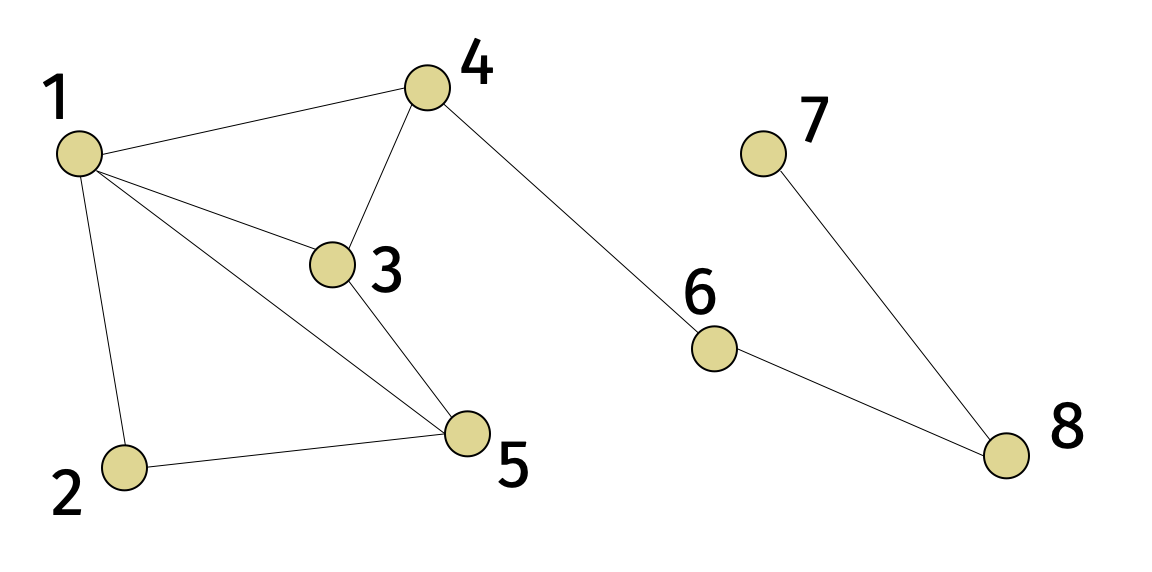
\includegraphics[width=.8\textwidth]{undirected_graph.png}
		
		For now assume $G = (V,E)$ is an undirected, unweighted graph with $n$ nodes.
	\end{center}
\end{frame}

\begin{frame}
	\frametitle{matrix representations of graphs}
	Two most common representations: $n\times n$ \emph{adjacency matrix} $\bv{A}$ and \emph{graph Laplacian} $\bv{L} = \bv{D}- \bv{A}$ where $\bv{D}$ is the diagonal degree matrix.
	\begin{center}
		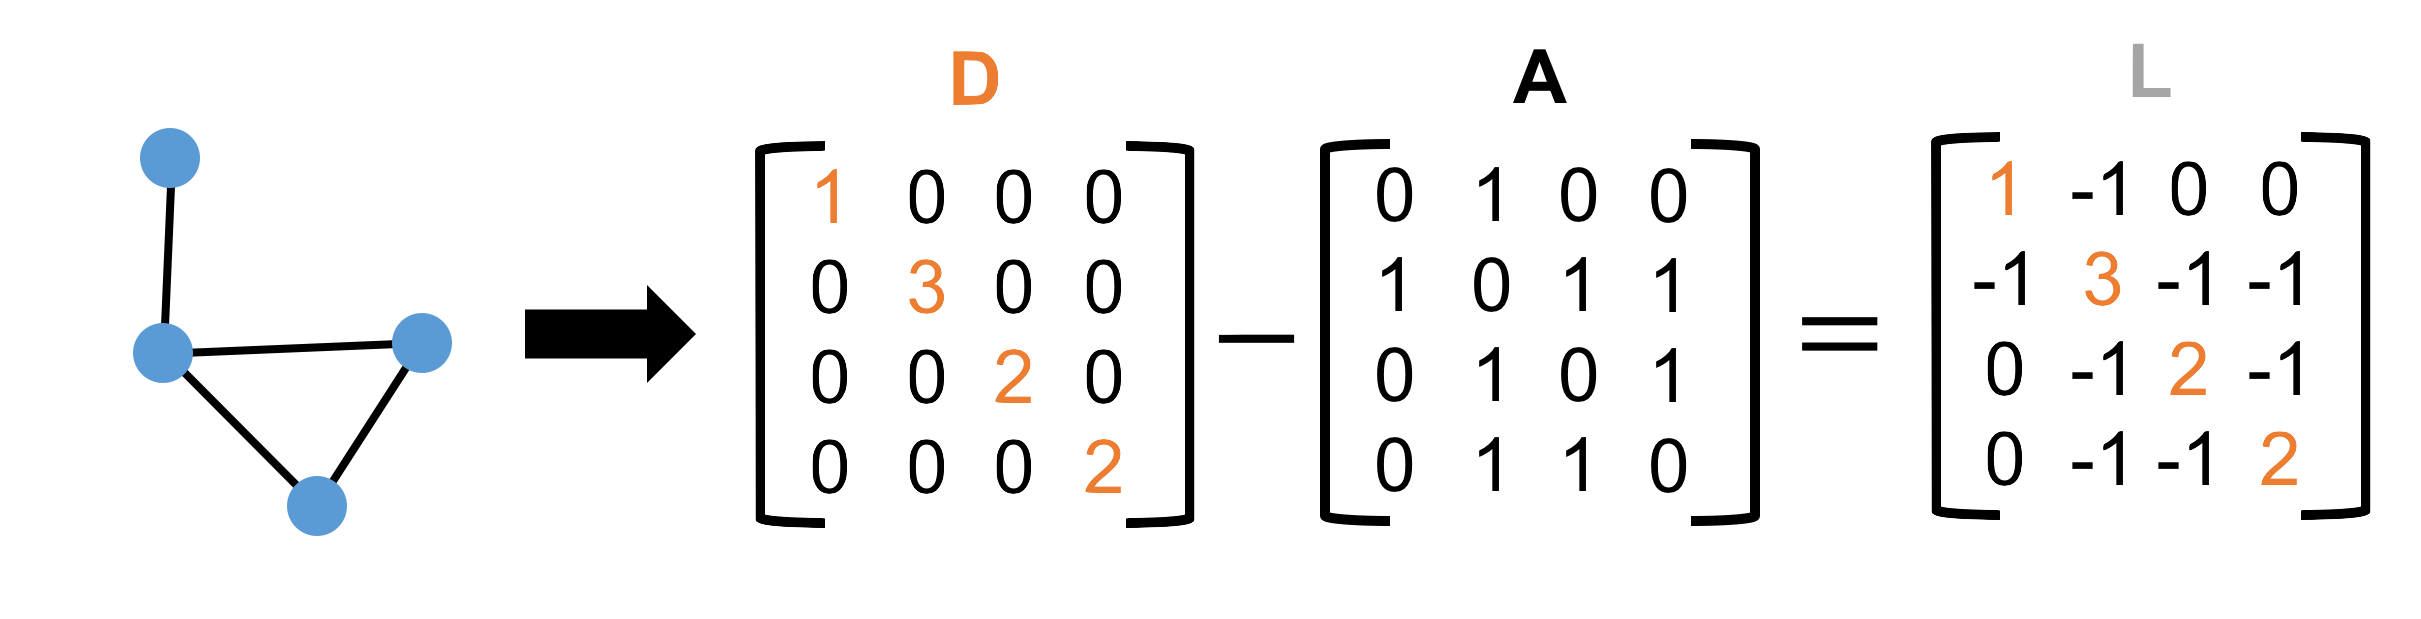
\includegraphics[width=\textwidth]{laplace.png}
	\end{center}

	Also common to look at normalized versions of both of these: $\bar{\bv{A}} = \bv{D}^{-1/2}\bv{A}\bv{D}^{-1/2}$ and $\bar{\bv{L}} = \bv{I} - \bv{D}^{-1/2}\bv{A}\bv{D}^{-1/2}$. 
\end{frame}


\begin{frame}[t]
	\frametitle{matrix representations of graphs}
		\frametitle{the laplacian view}
		\begin{center}
			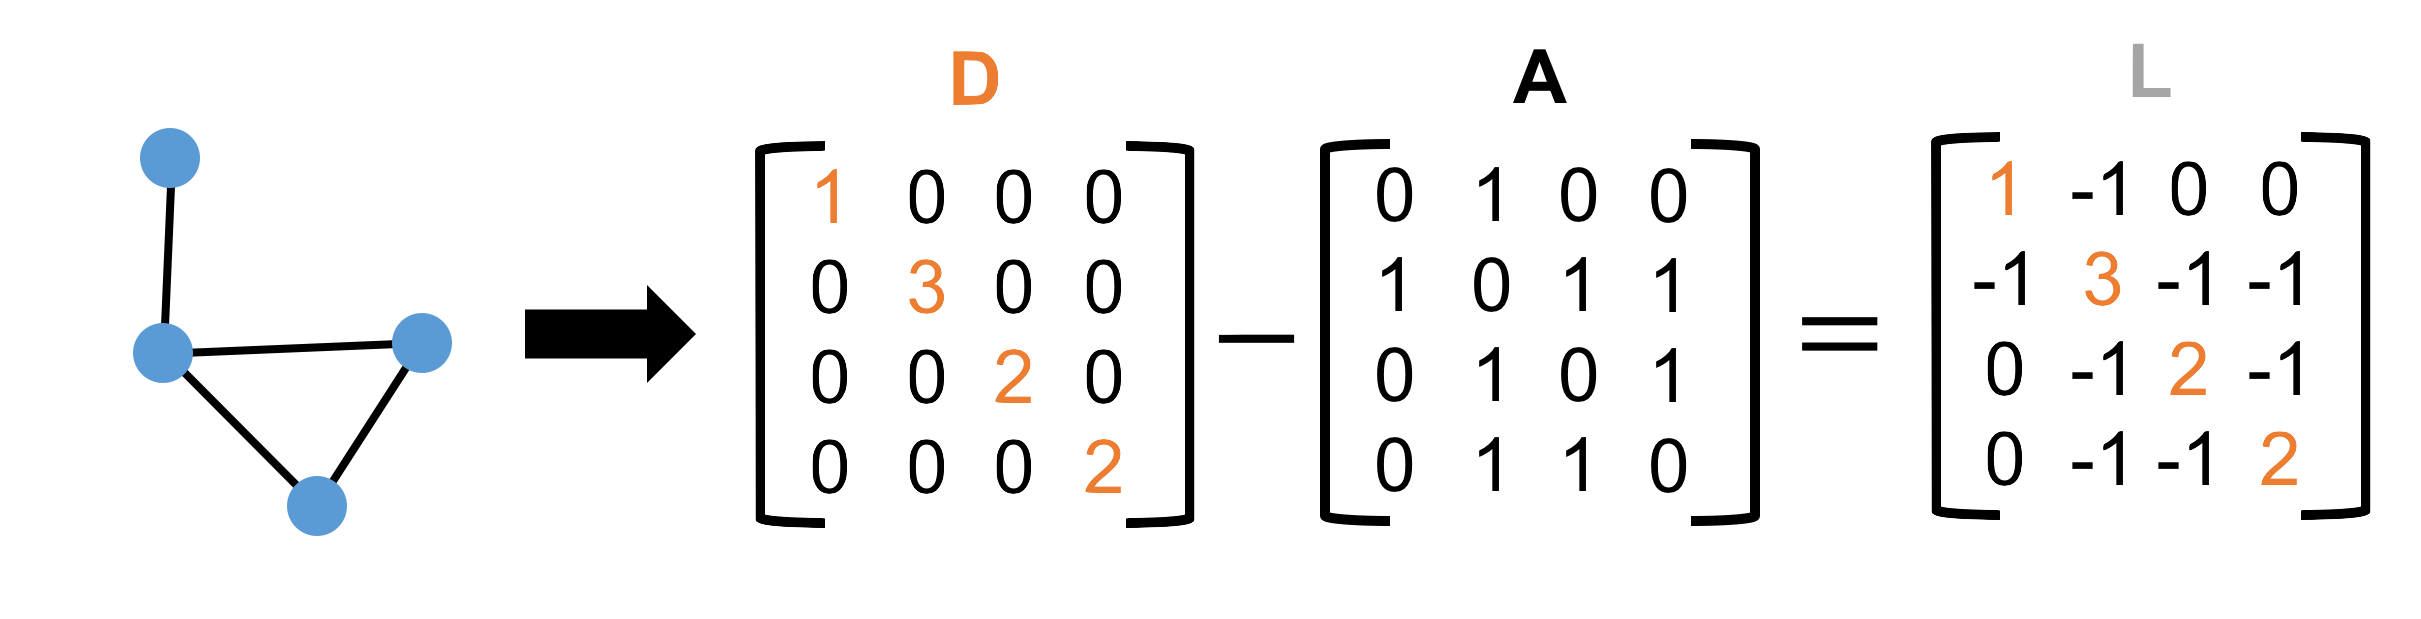
\includegraphics[width=.95\textwidth]{laplace.png}
			
			$\bv{L} = \bv{B}^T\bv{B}$ where $B$ is the signed ``edge-vertex incidence'' matrix.
		\end{center}
		$\bv{B}$ has a row for every edge in $G$. The row for edge $(i,j)$ has a $+1$ at position $i$, a $-1$ at position $j$, and zeros elsewhere. 	
\end{frame}


\begin{frame}[t]
	\frametitle{the laplacian view}
	\textbf{Conclusions from $\bv{L} = \bv{B}^T\bv{B}$}
	\begin{itemize}
		\item $\bv{L}$ is positive semidefinite: $\bv{x}^T\bv{L}\bv{x} \geq 0$ \emph{for all} $\bv{x}$. 
		\vspace{1em}
		\item $\bv{L} = \bv{V}\bs{\Sigma}^2\bv{V}^T$ where $\bv{U}\bs{\Sigma}\bv{V}^T$ is $\bv{B}$'s SVD. Columns of $\bv{V}$ are \emph{eigenvectors} of $\bv{L}$.
		\vspace{1em}
		\item 	\alert{For any vector $\bv{x}\in \R^n$, 
		\begin{align*}
			\bv{x}^T L \bv{x} = \sum_{(i,j)  \in E} (\bv{x}(i)- \bv{x}(j))^2. 
		\end{align*}}
	\end{itemize}	
\end{frame}

\begin{frame}[t]
	\frametitle{the laplacian view}
	$\bv{x}^T L \bv{x} = \sum_{(i,j)  \in E} (\bv{x}(i)- \bv{x}(j))^2$. So $\bv{x}^T L \bv{x}$ is small if $\bv{x}$ is a ``smooth'' function with respect to the graph. 
	\begin{center}
		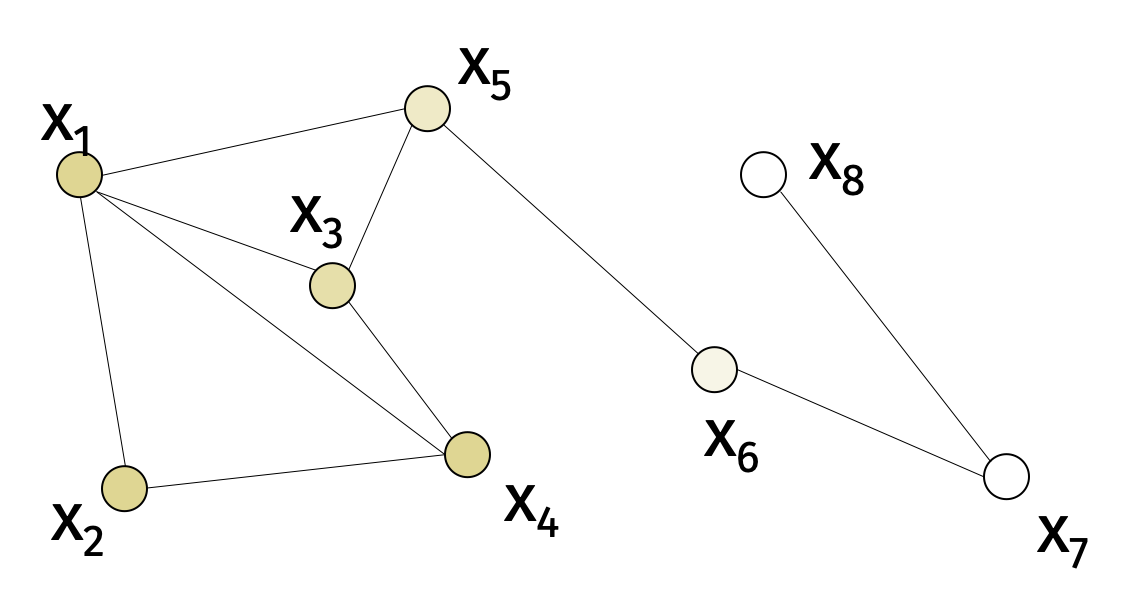
\includegraphics[width=.8\textwidth]{smooth_func.png}
	\end{center}
\end{frame}

\begin{frame}[t]
	\frametitle{the laplacian view}
	\textbf{Another conclusion from $\bv{L} = \bv{B}^T\bv{B}$}:
	
	For a \emph{cut indicator vector} $\bv{c} \in \{-1,1\}^n$ with $\bv{c}(i) = -1$ for $i \in S$ and $\bv{c}(i) = 1$ for $i \in T = V \setminus S$:
		\begin{align}
			 \bv{c}^T L \bv{c} = \sum_{(i,j)  \in E} (\bv{c}(i)- \bv{c}(j))^2 = 4 \cdot \cut(S,T).
		\end{align}
	
	\begin{center}
		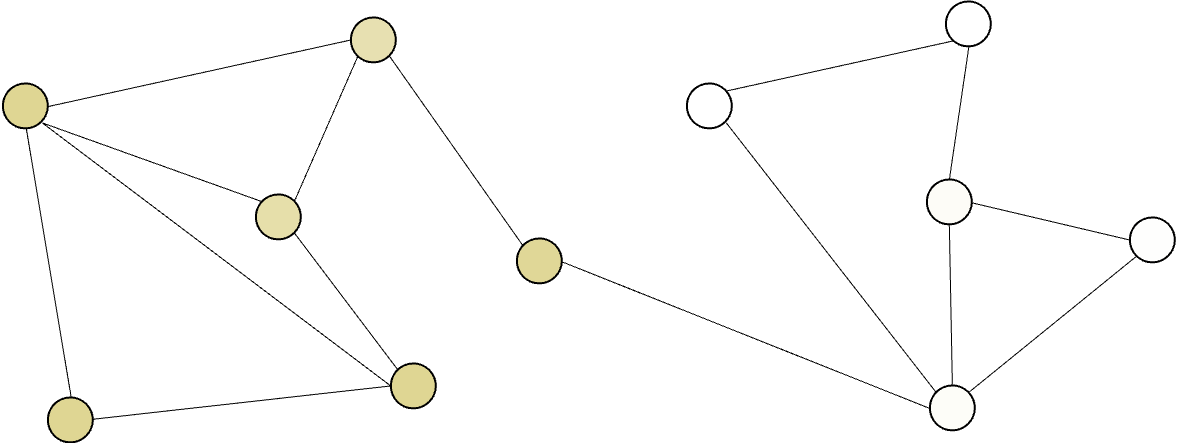
\includegraphics[width=.8\textwidth]{smooth_func2.png}
	\end{center}
\end{frame}

% \begin{frame}
% 	\frametitle{smallest laplacian eigenvector}
% 	\begin{center}
% 		\textbf{Courant–Fischer min-max principle}
% 	\end{center}
% 	Let $\bv{V} = [\bv{v}_1,\ldots,\bv{v}_n]$ be the eigenvectors of $\bv{L}$.
	
% 	\begin{align*}
% 		\bv{v}_n &= \argmin_{\|\bv{v}\|=1} \bv{v}^T\bv{L}\bv{v} \\
% 		\bv{v}_{n-1} &= \argmin_{\|\bv{v}\|=1,\bv{v} \perp \bv{v}_n} \bv{v}^T\bv{L}\bv{v} \\
% 		\bv{v}_{n-2}  &= \argmin_{\|\bv{v}\|=1,\bv{v} \perp \bv{v}_n,\bv{v}_{n-1}} \bv{v}^T\bv{L}\bv{v} \\
% 		&\vdots \\
% 		\bv{v}_1 &= \argmin_{\|\bv{v}\|=1,\bv{v} \perp \bv{v}_n,\ldots,\bv{v}_2} \bv{v}^T\bv{L}\bv{v} 
% 	\end{align*}
% \end{frame}

% \begin{frame}
% 	\frametitle{largest laplacian eigenvector}
% 	\begin{center}
% 		\textbf{Courant–Fischer min-max principle}
% 	\end{center}
% 	Let $\bv{V} = [\bv{v}_1,\ldots,\bv{v}_n]$ be the eigenvectors of $\bv{L}$.
	
% 	\begin{align*}
% 		\bv{v}_1 &= \argmax_{\|\bv{v}\|=1} \bv{v}^T\bv{L}\bv{v} \\
% 		\bv{v}_2 &= \argmax_{\|\bv{v}\|=1,\bv{v} \perp \bv{v}_1} \bv{v}^T\bv{L}\bv{v} \\
% 		\bv{v}_3 &= \argmax_{\|\bv{v}\|=1,\bv{v} \perp \bv{v}_1,\bv{v}_2} \bv{v}^T\bv{L}\bv{v} \\
% 		&\vdots \\
% 		\bv{v}_n &= \argmax_{\|\bv{v}\|=1,\bv{v} \perp \bv{v}_1,\ldots,\bv{v}_{n-1}} \bv{v}^T\bv{L}\bv{v} 
% 	\end{align*}
% \end{frame}

\begin{frame}
	\frametitle{spectral graph partitioning}
	\begin{itemize}
		\item Introduce NP-hard \emph{graph partitioning} problem important in:
		\begin{itemize}
			\item Understanding social networks. 
			\item Unsupervised machine learning (spectral clustering).
			\item Graph visualization. 
			\item Mesh partitioning.
		\end{itemize}
		\item See how this problem can be solved heuristically using Laplacian eigenvectors. 
		\item Give an ``average case'' analysis of the method for a common \emph{random graph model}.
		\item Use two tools: \emph{matrix concentration} and \emph{eigenvector perturbation bounds}.
	\end{itemize}
\end{frame}


\begin{frame}
	\frametitle{balanced cut}
	\textbf{Goal:} Given a graph $G = (V,E)$, partition nodes along a cut that:
	\begin{itemize}
		\item Has few crossing edges: $|\{(u,v) \in E: u\in S,v\in T \}|$ is small.
		\item Separates large partitions: $|S|,|T|$ are not too small.
	\end{itemize}
\vspace{-.5em}
	\begin{center}
		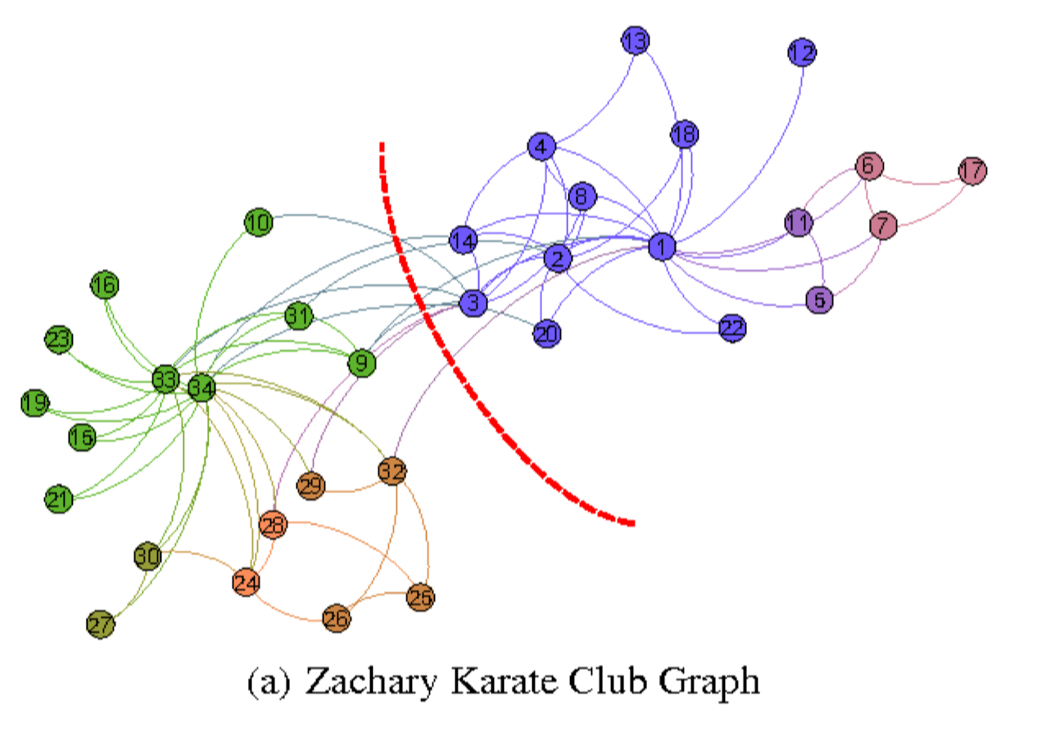
\includegraphics[width=.55\textwidth]{karate.png}
		\vspace{-1em}
	\end{center}
	\textbf{Example application:} Understanding \emph{community structure} in social networks. 
\end{frame}

\begin{frame}
	\frametitle{social networks in the 1970s}
	\begin{center}
	Wayne W. Zachary (1977). An Information Flow Model for Conflict and Fission in Small Groups.
	\end{center}
	
	\small{
	``At the beginning of the study there was an incipient conflict
	between the club president, John A., and Mr. Hi over the price of
	karate lessons. Mr. Hi, who wished to raise prices, claimed the authority
	to set his own lesson fees, since he was the instructor. John A., who
	wished to stabilize prices, claimed the authority to set the lesson fees
	since he was the club's chief administrator.
	As time passed the entire club became divided over this issue, and
	the conflict became translated into ideological terms by most club
	members.''
}
	
	\begin{center}
		\textbf{Zachary constructed a social network by hand and used a minimum cut algorithm to correctly predict who sided with who in the conflict. 
		\alert{Beautiful paper -- definitely worth checking out!}}
	\end{center}
\end{frame}



\begin{frame}
	\frametitle{spectral clustering}
	\textbf{Idea:} Construct synthetic graph for data that is hard to cluster.
	
	\begin{center}
		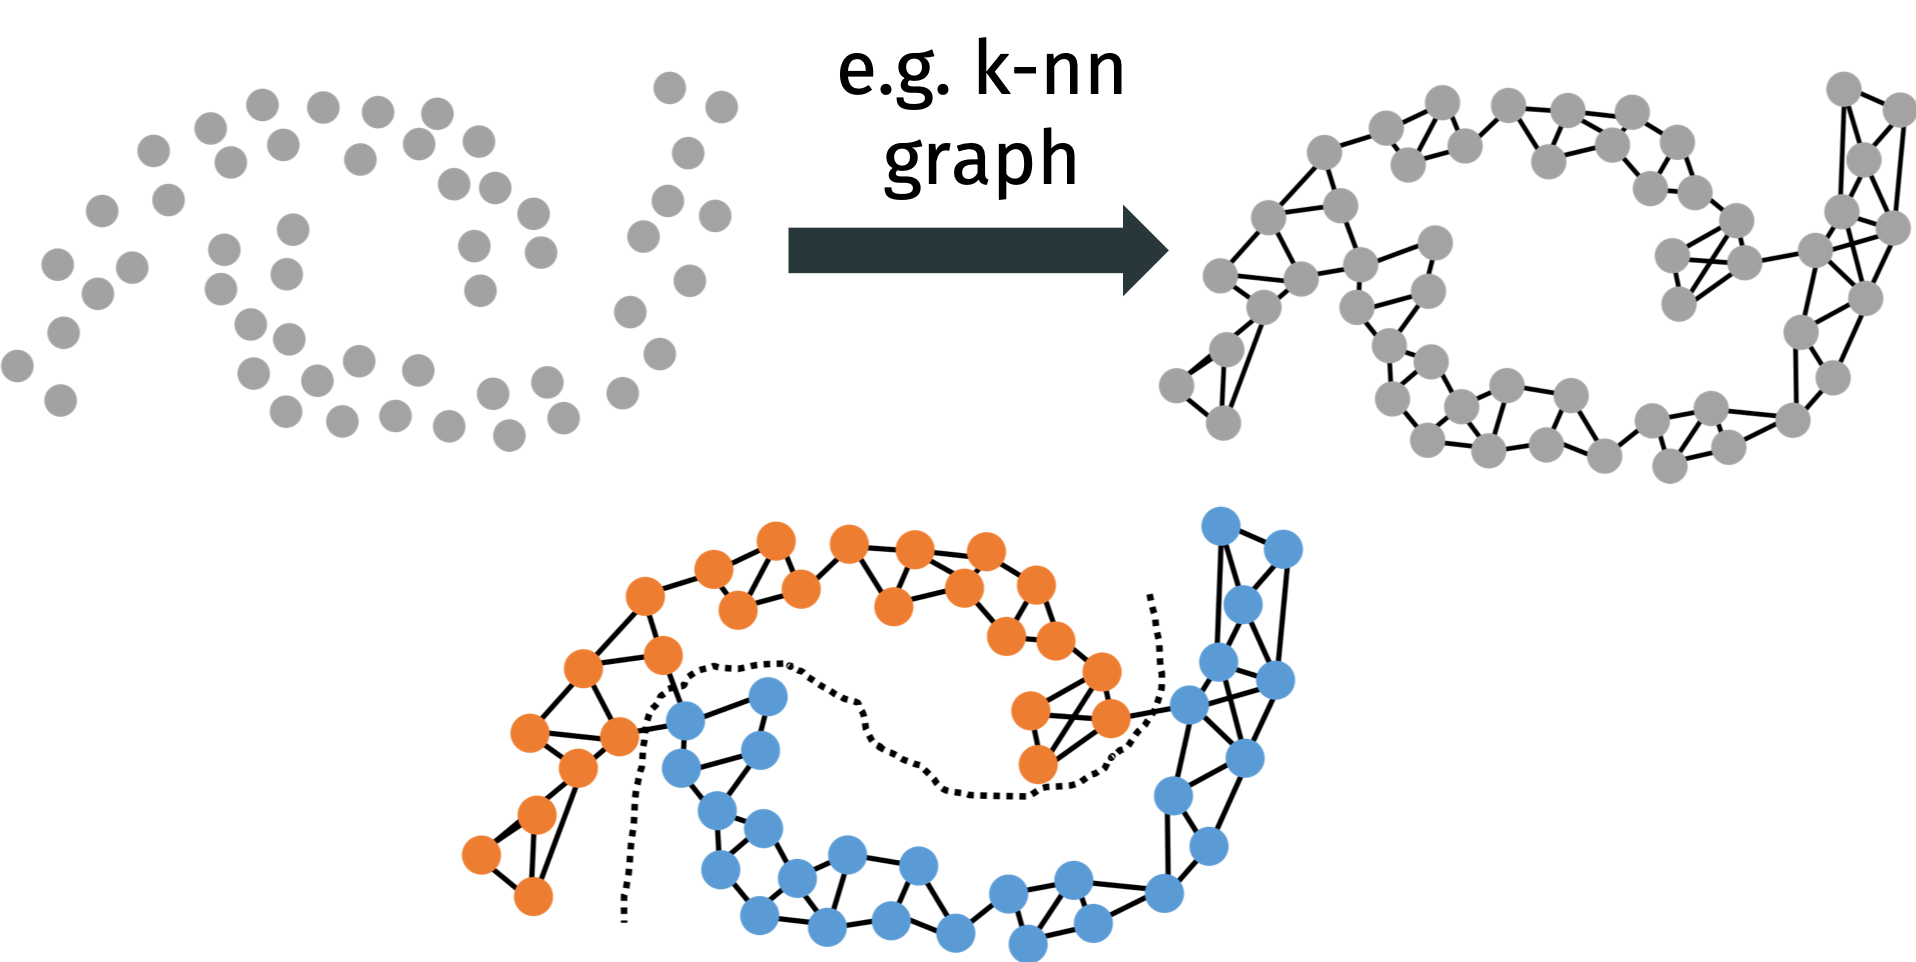
\includegraphics[width=\textwidth]{cut_clustering.png}
		
		Spectral Clustering, Laplacian Eigenmaps, Locally linear embedding, Isomap, etc.
	\end{center}
	
\end{frame}

\begin{frame}
	\frametitle{tons of other applications!}
	Balanced cut algorithms are also use in distributing data in graph databases, for partitioning finite element meshes in scientific computing (e.g., that arise when solving differential equations), and more. 
	
	\begin{center}
	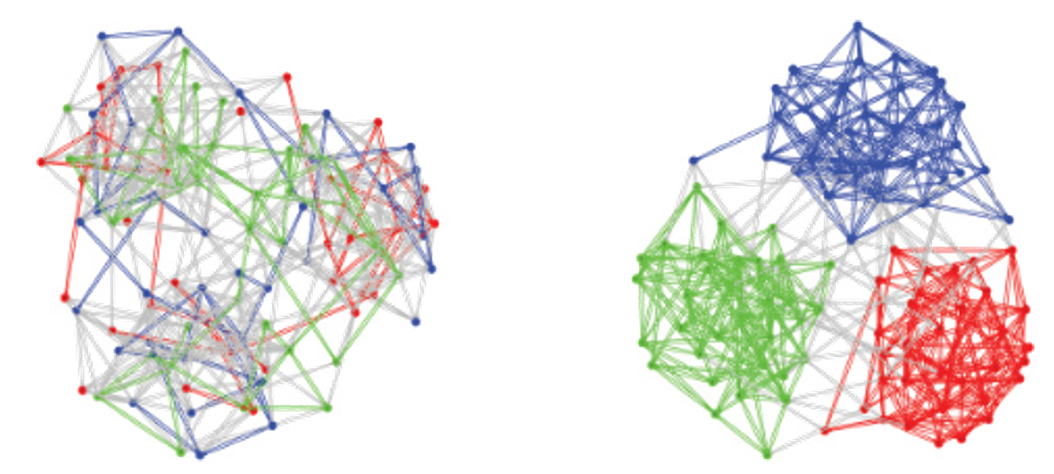
\includegraphics[height=.3\textheight]{balanced_partition.png} \hfill	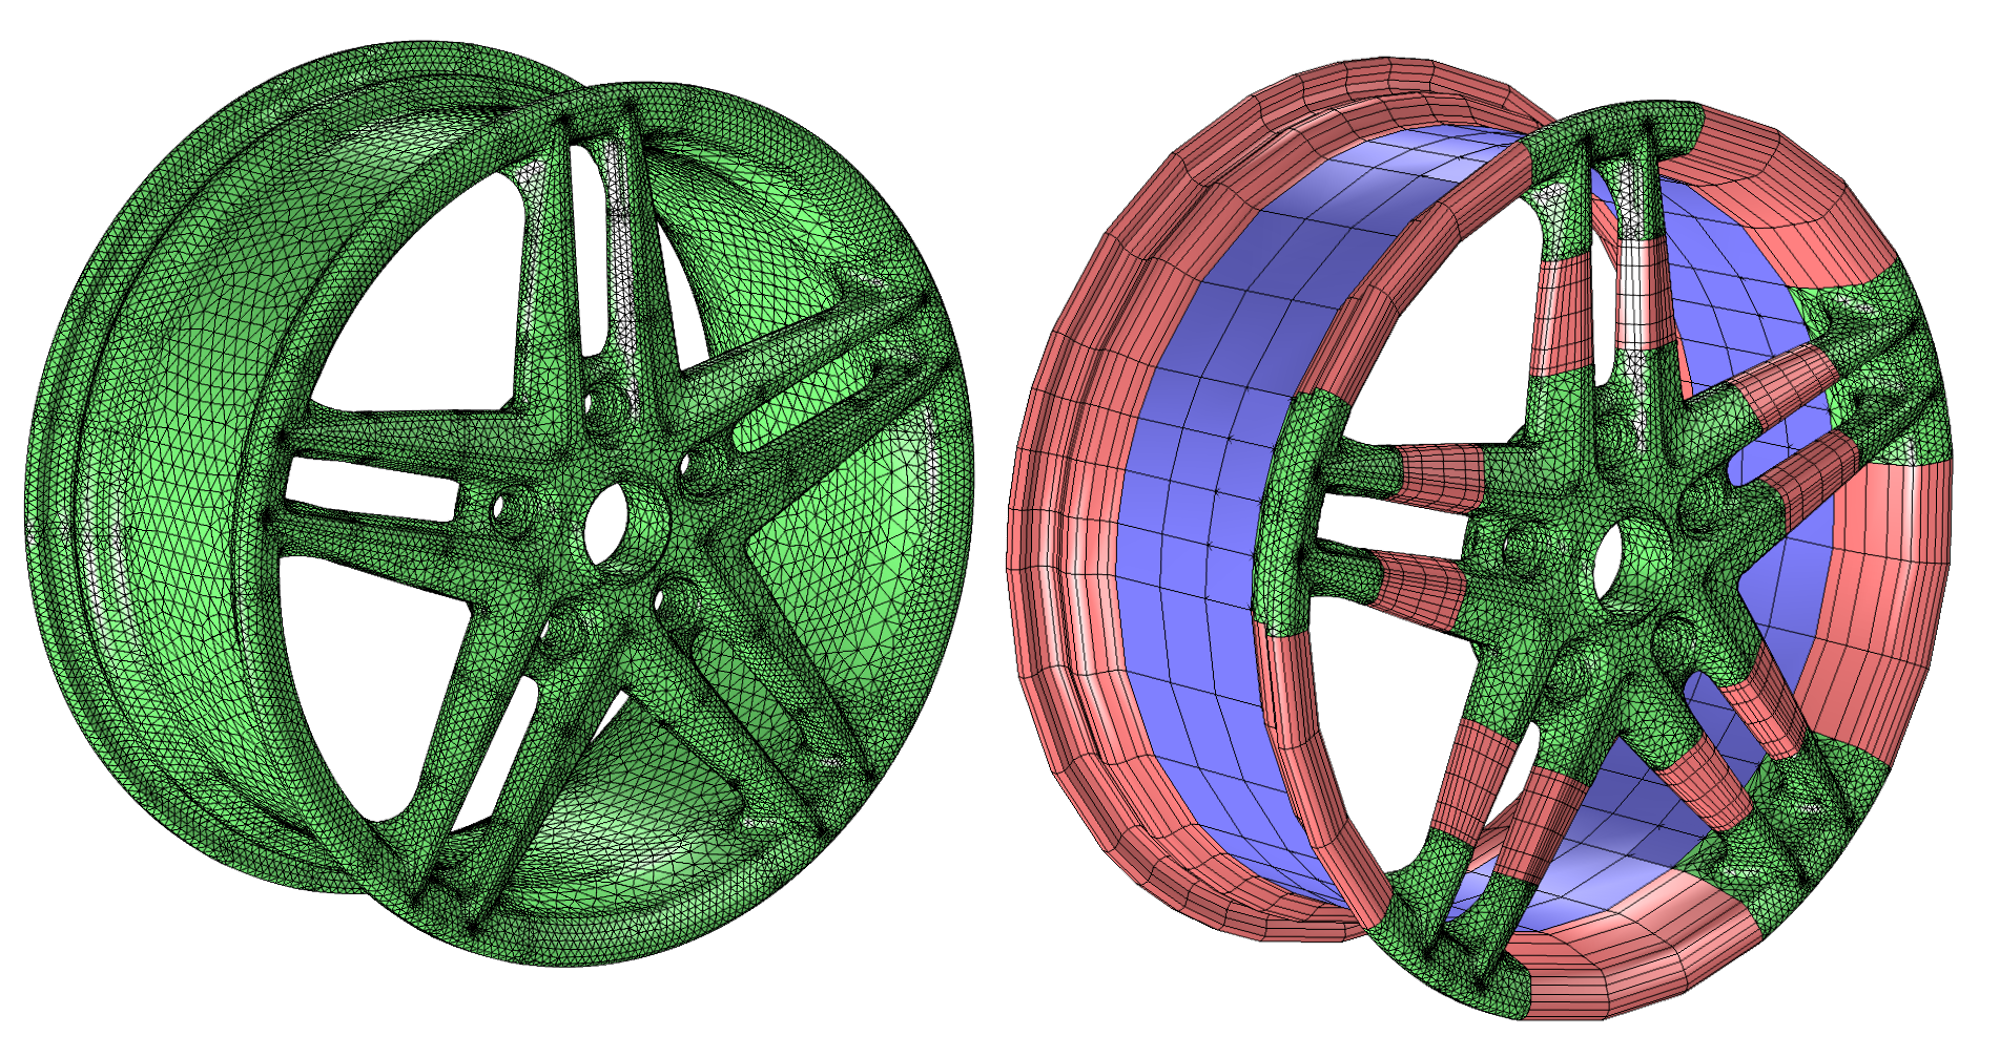
\includegraphics[height=.3\textheight]{finite_element_1.png}
	
	Lots of good software packages (e.g. METIS). 
	\end{center}
\end{frame}

\begin{frame}[t]
	\frametitle{spectral graph partitioning}
	There are many way's to formalize Zachary's problem:
	
		\textbf{$\beta$-Balanced Cut:}
	\begin{align*}
		&\min_{S} {\cut(S, V\setminus S)} & &\text{such that} & &\min\left(|S|,|V\setminus S|\right) \geq \beta\cdot n \text{ for } \beta \leq .5
	\end{align*}
	
	\textbf{Sparsest Cut:}
	\begin{align*}
		\min_{S} \frac{\cut(S, V\setminus S)}{\min\left(|S|,|V\setminus S|\right)}
	\end{align*}



	All natural formalizations lead to NP-hard problems. Lots of interest in designing polynomial time approximation algorithms, but tend to be slow. In practice, much simpler methods based on the \emph{graph spectrum} are used. 
	
	\begin{center}
		\textbf{Spectral  methods run no more than $O(n^3)$ time (must faster if you use iterative methods for computing eigenvectors).}
	\end{center}
\end{frame}

\begin{frame}
		\frametitle{spectral graph partitioning}
	\textbf{Basic spectral clustering method:}
	\begin{itemize}
		\item Compute \emph{second} smallest eigenvector of graph, $\bv{v}_{n-1}$.
		\item $\bv{v}_{n-1}$ has an entry for every node $i$ in the graph.
		\item If the $i^{\text{th}}$ entry is positive, put node $i$ in $T$.
		\item Otherwise if the $i^{\text{th}}$ entry is negative, put $i$ in $S$.
	\end{itemize}	
\begin{center}
	\textbf{\alert{This shouldn't make much sense yet!} We will see that is a ``relax and round'' algorithm in disguise.}
\end{center}
\end{frame}

\begin{frame}
	\frametitle{the laplacian view}
	\begin{center}
	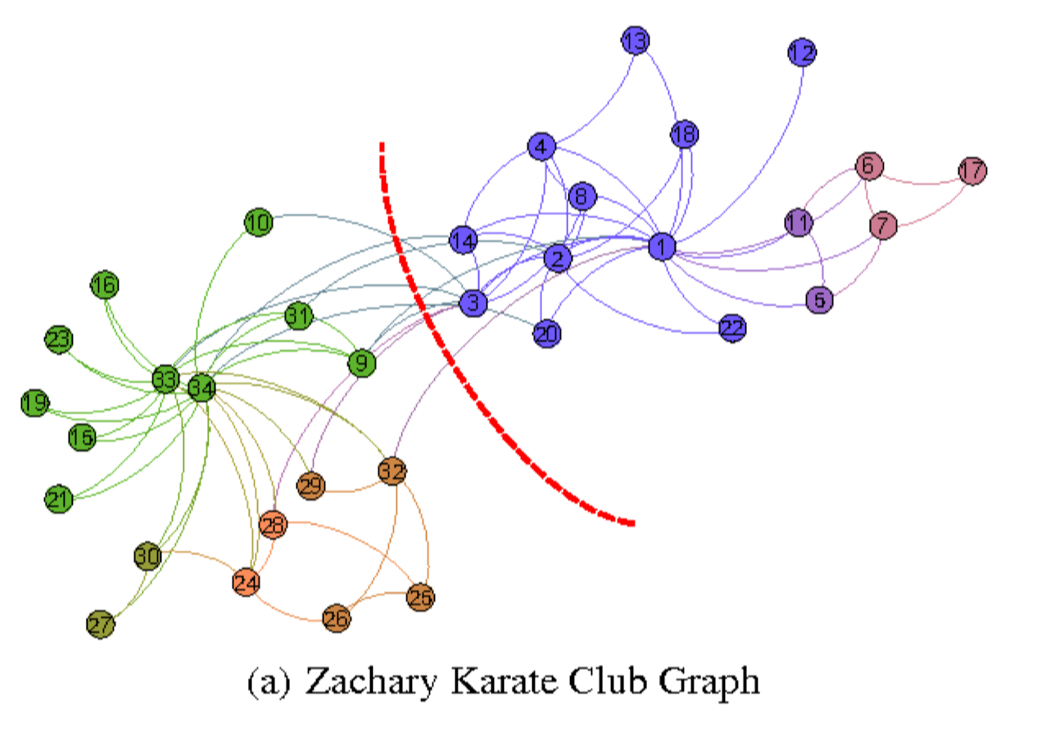
\includegraphics[width=.4\textwidth]{karate.png}
	\end{center}
	For a \emph{cut indicator vector} $\bv{c} \in \{-1,1\}^n$ with $\bv{c}(i) = -1$ for $i \in S$ and $\bv{c}(i) = 1$ for $i \in T$:
	\begin{itemize}
		\item $\bv{c}^T L \bv{c} = 4 \cdot cut(S,T)$.
		\item $\bv{c}^T \bv{1} = |T| - |S|$.
	\end{itemize}
	Want to minimize both $\bv{c}^T L \bv{c}$ (cut size) and $|\bv{c}^T \bv{1}|$ (imbalance).
\end{frame}

\begin{frame}
	\frametitle{the laplacian view}
	\begin{center}
		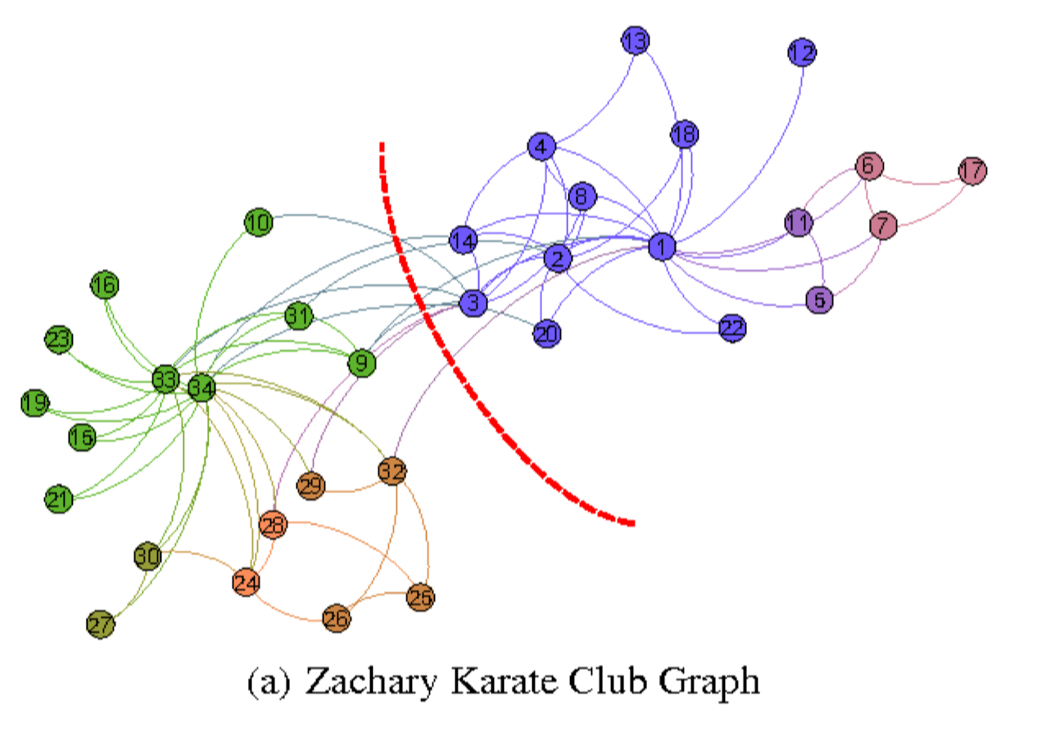
\includegraphics[width=.4\textwidth]{karate.png}
	\end{center}
	Equivalent formulation if we divide everything by $\sqrt{n}$ so that $\bv{c}$ has norm $1$. Then $\bv{c} \in \{-\frac{1}{\sqrt{n}},\frac{1}{\sqrt{n}}\}^n$ and:
	\begin{itemize}
		\item $\bv{c}^T L \bv{c} = \frac{4}{n} \cdot cut(S,T)$.
		\item $\bv{c}^T \bv{1} = \frac{1}{\sqrt{n}}(|T| - |S|)$.
	\end{itemize}
	Want to minimize both $\bv{c}^T L \bv{c}$ (cut size) and $|\bv{c}^T \bv{1}|$ (imbalance).
\end{frame}

\begin{frame}
	\frametitle{relax and round}
	\textbf{Perfectly balanced balanced cut problem:}
	\begin{align*}
		\min_{\bv{c} \in \{-\frac{1}{\sqrt{n}},\frac{1}{\sqrt{n}}\}^n} \bv{c}^T\bv{L}\bv{c} \text{ such that } \bv{c}^T\bv{1} = 0.
	\end{align*}

	\textbf{Relaxed perfectly balanced balanced cut problem:}
	\begin{align*}
		\min_{\|\bv{c}\|_2 = 1} \bv{c}^T\bv{L}\bv{c} \text{ such that } \bv{c}^T\bv{1} = 0.
	\end{align*}

	\textbf{Claim:} The relaxed problem is exactly minimized by the second smallest eigenvector $\bv{v}_{n-1}$ of $\bv{L}$. 

	\textbf{Approach:} Relax, find $\bv{v}_{n-1}$, then round back to a vector with $-\frac{1}{\sqrt{n}},\frac{1}{\sqrt{n}}$ entries.
\end{frame}




\begin{frame}[t]
	\frametitle{smallest laplacian eigenvector}
	\textbf{Claim:} The smallest eigenvector/singular vector of any graph Laplacian $\bv{L}$ always equals:
	\begin{align*}
	\bv{v}_n = \argmin_{v \in \R^n\text{ with } \norm{\bv{v}} = 1} \bv{v}^T L \bv{v} = \frac{1}{\sqrt{n}} \cdot \bv{1}
	\end{align*}
	with $\bv{v}_n^T  L \bv{v}_n = 0$. 
	
	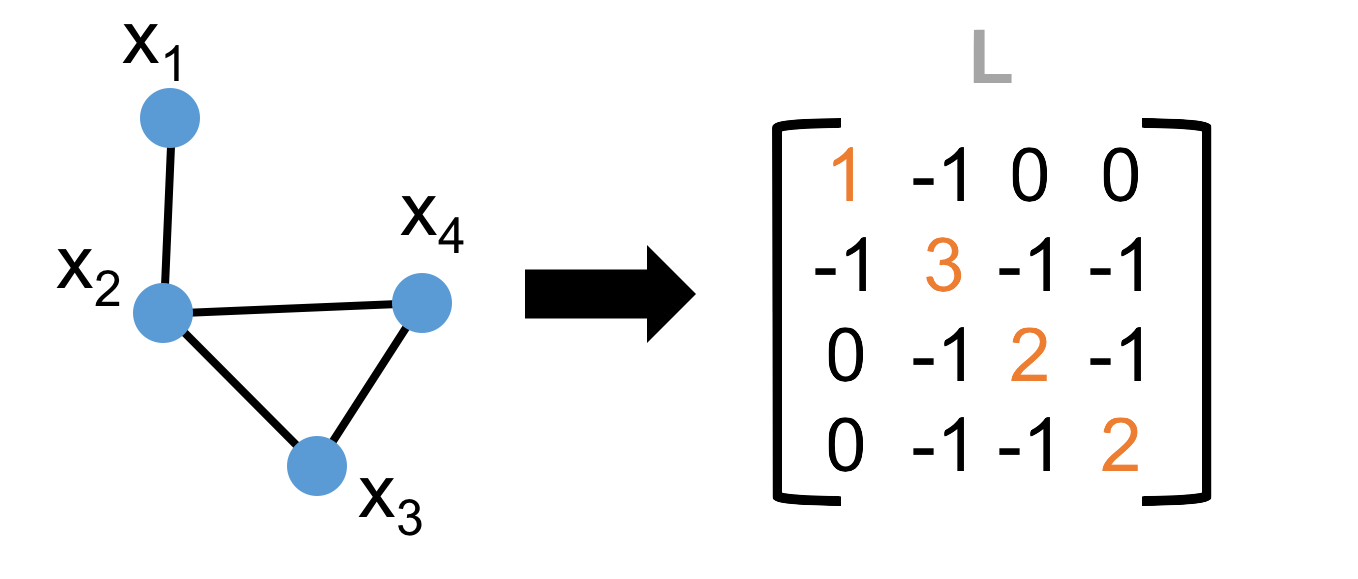
\includegraphics[width=.5\textwidth]{laplace_compact.png}
\end{frame}

\begin{frame}
	\frametitle{second smallest laplacian eigenvector}
	By Courant-Fischer, $\bv{v}_{n-1}$ is given by:
	\begin{align*}
	\bv{v}_{n-1} = \argmin_{\norm{\bv{v}} = 1,\ {\bv{v}_n^T \bv{v} = 0}} \bv{v}^T L \bv{v}
	\end{align*}
	which is equivalent to
	\begin{align*}
		\bv{v}_{n-1} = \argmin_{\norm{\bv{v}} = 1,\ {\bv{1}^T \bv{v} = 0}} \bv{v}^T L \bv{v}.
	\end{align*}
\end{frame}

\begin{frame}
	\frametitle{cutting with the  second laplacian eigenvector}
	\textbf{Final relax and round algorithm:} Compute 
	$$\bv{v}_{n-1} = \argmin_{v \in \R^n \text{ with } \norm{\bv{v}} = 1,\ \alert{\bv{v}^T \bv{1} = 0}} \bv{v}^T L \bv{v}$$ Set $S$ to be all nodes with $\bv{v}_{n-1}(i) < 0$, and $T$ to be all with $\bv{v}_{n-1}(i) \ge 0$. I.e. set $\bv{c} = \sign(\bv{v}_{n-1})$
	\begin{center}
		\vspace{-1em}
		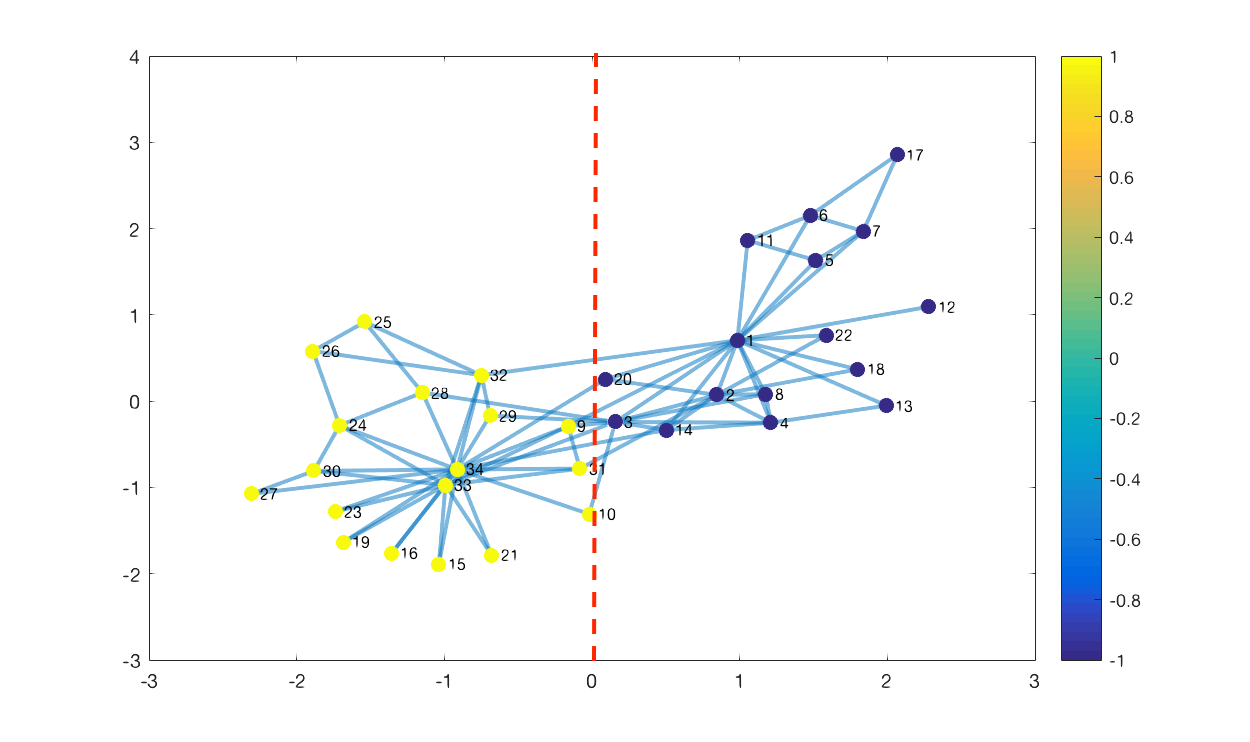
\includegraphics[width=.9\textwidth]{cut2-fix.png}
	\end{center}
\end{frame}

\begin{frame}
	\frametitle{spectral partitioning in practice}
	Lots of different variants used in practice:
	\begin{itemize}
		\item Often do some sort of normalization of edge weights by degree. E.g. the Shi-Malik normalized cuts algorithm use the normalized Laplacian $\mathbf{\overline L} = \bv{D}^{-1/2} \bv{L} \bv{D}^{-1/2}$.
		\item Different methods for how to choose the threshold to partition the second smallest eigenvector.
		\item Lots of variants to split the graph into more than two parts.
	\end{itemize}
		\begin{center}
				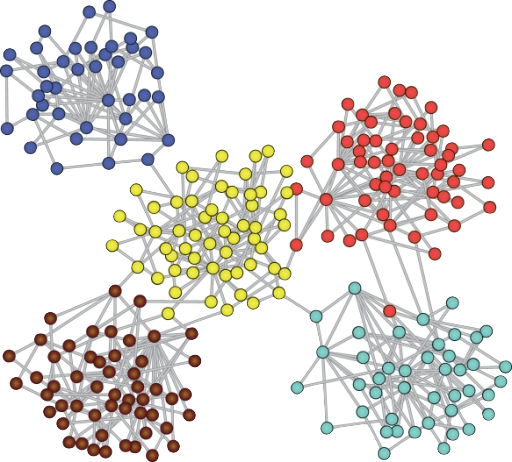
\includegraphics[width=.33\textwidth]{multiway.png}
		\end{center}
\end{frame}

\begin{frame}
	\frametitle{spectral partitioning in practice}
	\textbf{Multiway spectral partitioning:}
	\begin{itemize}
		\item Compute smallest $\ell$ eigenvectors $\bv{v}_{n-1}, \ldots, \bv{v}_{n-\ell}$ of $\mathbf{L}$.
		\item Represent each node by its corresponding row in $\bv{V} \in \R^{n \times \ell}$ whose rows are  $\bv{v}_{n-1}, \ldots \bv{v}_{n-\ell}$.
		\item Cluster these rows using $k$-means clustering (or really any clustering method).
		\item Often we choose $\ell = k$, but not necessarily. 
	\end{itemize}
\end{frame}

\begin{frame}
	\frametitle{laplacian embedding}
	\begin{center}
		\textbf{Original Data:} (not linearly separable)
			
			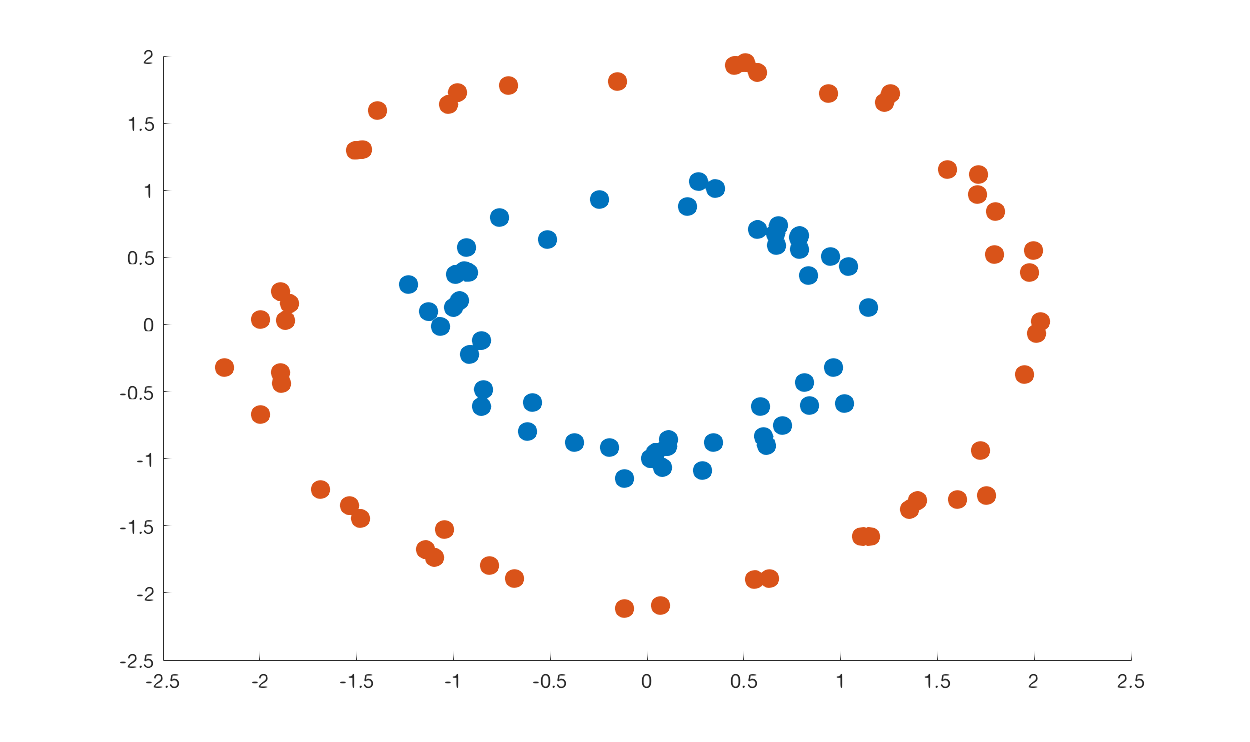
\includegraphics[width=.7\textwidth]{circ.png}
	\end{center}
\end{frame}

\begin{frame}
	\frametitle{laplacian embedding}
	\begin{center}
			\textbf{$k$-Nearest Neighbors Graph:}
			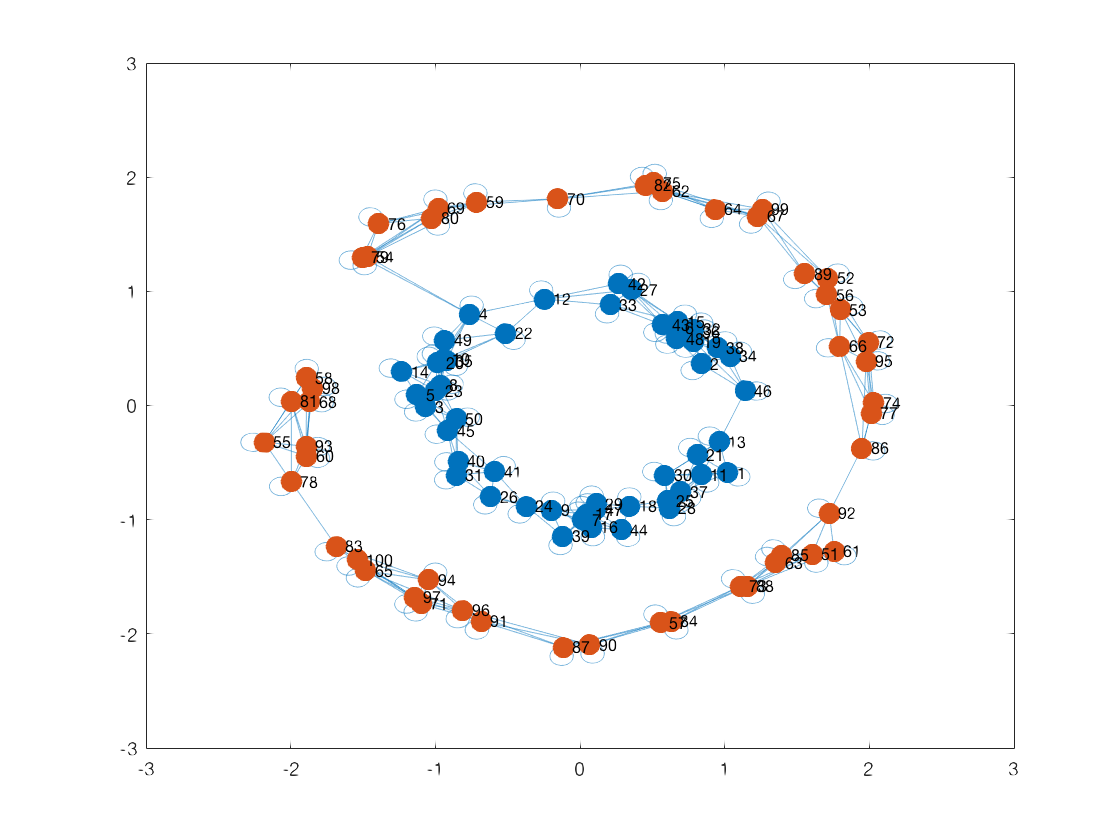
\includegraphics[width=.7\textwidth]{circ2.png}
	\end{center}
\end{frame}

\begin{frame}
	\frametitle{laplacian embedding}
	\begin{center}
	\textbf{Embedding with eigenvectors $\bv{v}_{n-1}, \bv{v}_{n-2}$:} (linearly separable) 
			
			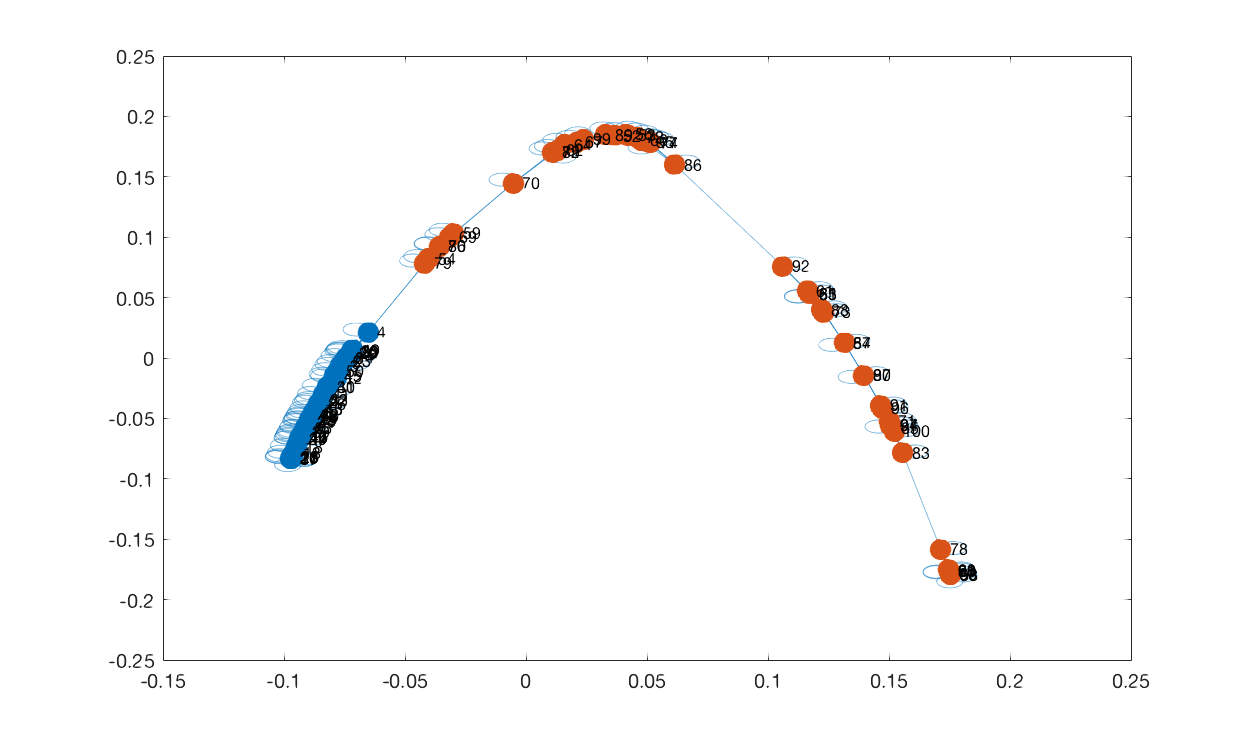
\includegraphics[width=.7\textwidth]{circ3.png}
	\end{center}
\end{frame}

\begin{frame}
	\frametitle{why does this work?}
	Intuitively, since $\bv{v} \in \bv{v}_{n-1}, \ldots \bv{v}_{n-\ell}$ are smooth over the graph, 
	\begin{align*}
		\sum_{i,j \in E} (\bv{v}[i] - \bv{v}[j])^2
	\end{align*}
	is small for each coordinate. I.e. this embedding explicitly encourages nodes connected by an edge to be placed in nearby locations in the embedding.
	\begin{center}
		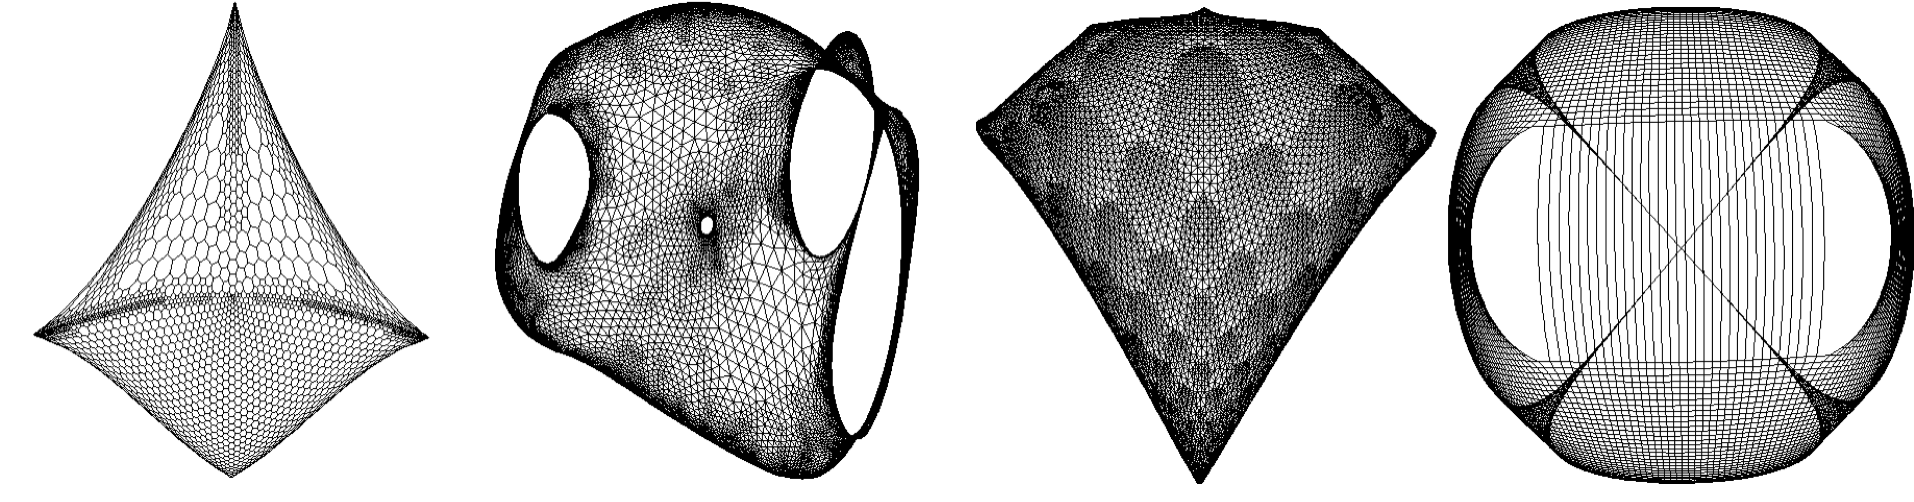
\includegraphics[width=\textwidth]{graph_drawing.png}
		
		Also useful e.g., in graph drawing.
	\end{center}
	
\end{frame}

\begin{frame}
	\frametitle{generative models}
	\textbf{So far:} Showed that spectral clustering partitions a graph along a small cut between large pieces.   
	\begin{itemize}
		\item No formal guarantee on the `quality' of the partitioning.
		\item Can fail for worst case input graphs.
	\end{itemize}
	\textbf{Common approach:} Design a natural \alert{\textbf{generative model}} that produces \emph{random but realistic} inputs and analyze how the algorithm performs on inputs drawn from this model.
	\begin{itemize}
		\item Very common in algorithm design and analysis. Great way to start approaching a problem. Often our best way to understand why some algorithms ``just work'' in practice.
		\item Similar approach to Bayesian modeling in machine learning.
	\end{itemize}
\end{frame}


\begin{frame}[t]
	\frametitle{stochastic block model}
	\begin{center}
		\alert{Ideas for a generative model for \textbf{social network graphs} that would allow us to understand partitioning?}
	\end{center}
	
\end{frame}

\begin{frame}
	\frametitle{stochastic block model}
	\textbf{Stochastic Block Model (Planted Partition Model):} 
	
	Let $G_n(p,q)$ be a distribution over graphs on $n$ nodes, split equally into two groups $B$ and $C$, each with $n/2$ nodes.
	\begin{itemize}
		\item Any two nodes in the \textbf{\alert{same group}} are connected with probability $p$ (including self-loops).
		\item Any two nodes in \textbf{\alert{different groups}} are connected with prob. $q < p$.
	\end{itemize}
	\vspace{-1em}
	\begin{center}
		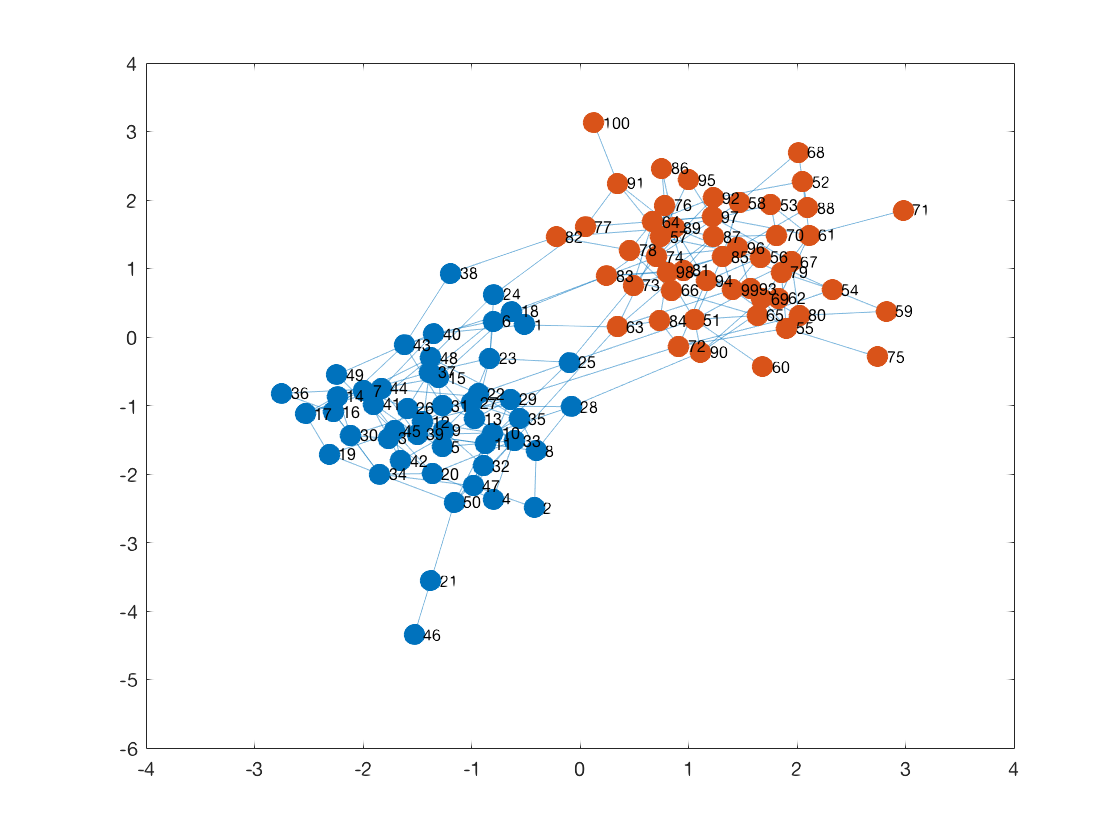
\includegraphics[width=.5\textwidth]{stochasticBlock.png}
	\end{center}
\end{frame}

\begin{frame}
	\frametitle{linear algebraic view}
	Let $G$ be a stochastic block model graph drawn from $G_n(p,q)$. 
	\begin{itemize}
		\item Let $\bv A \in \R^{n \times n}$ denote the adjacency matrix of $G$.
		\begin{center}
			\hspace{-3em}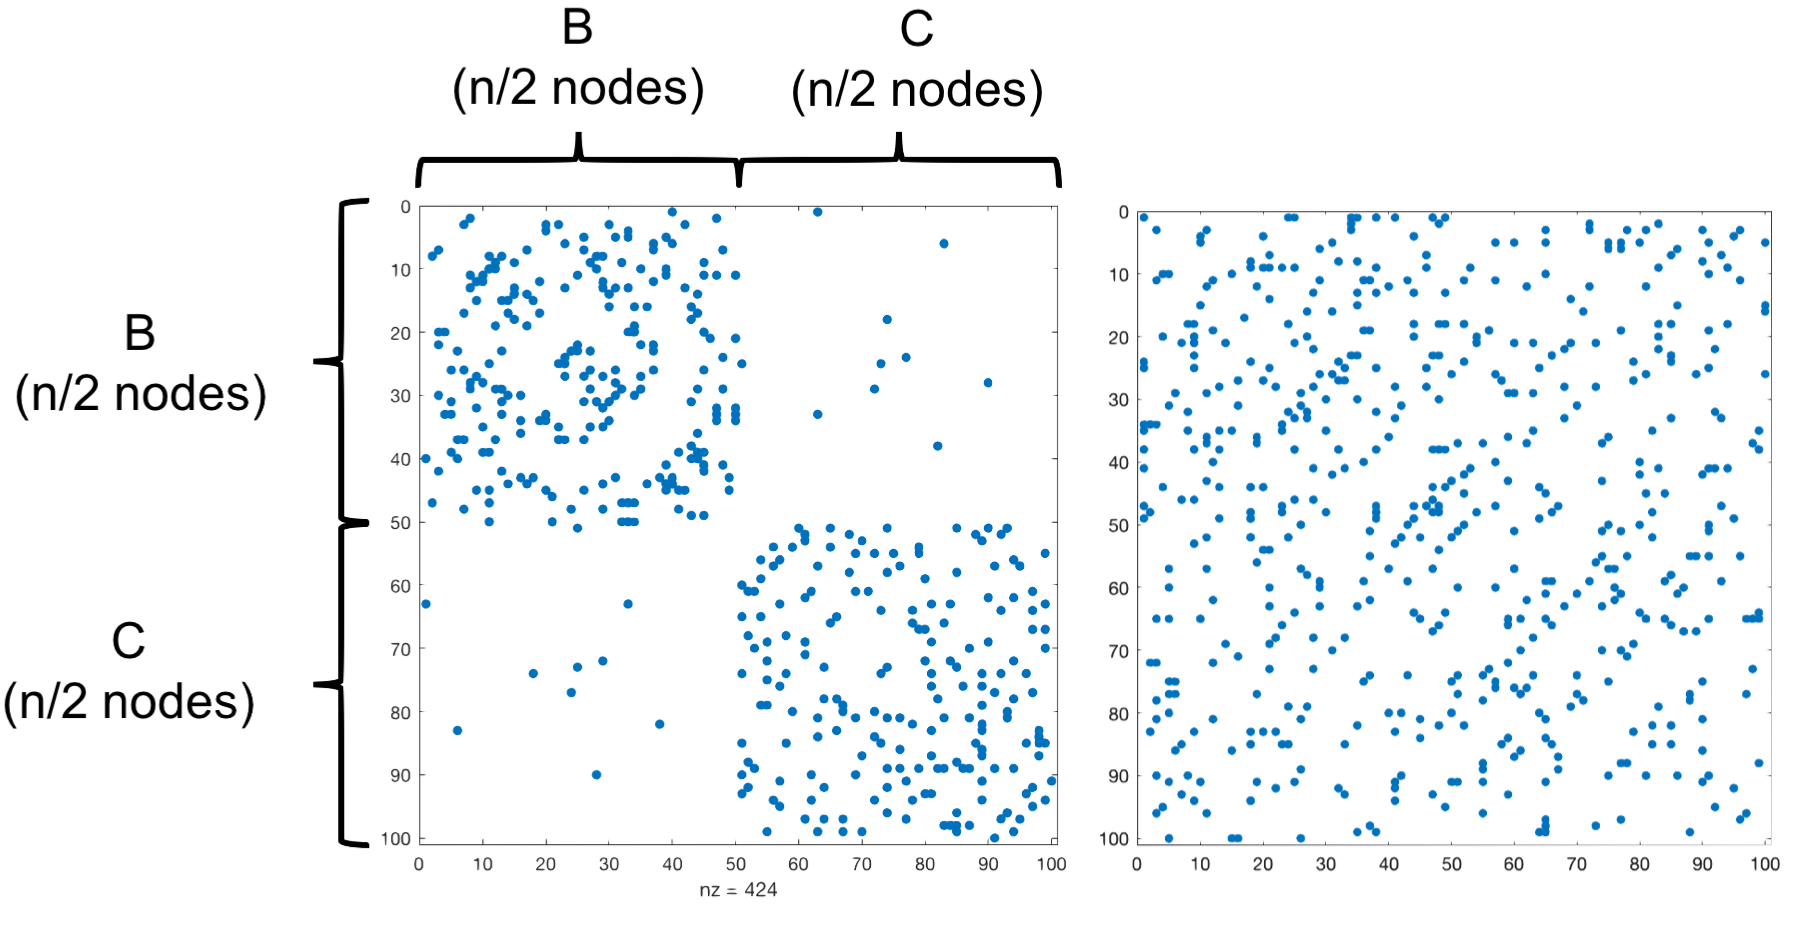
\includegraphics[width=.9\textwidth]{scrambled.png}
		\end{center}
	\end{itemize}
	\textbf{Note that we are \emph{arbitrarily} ordering the nodes in $\bv{A}$ by group. In reality $\bv{A}$ would look ``scrambled'' as on the right.}
\end{frame}

\begin{frame}
	\frametitle{stochastic block model}
	Goal is to find the ``ground truth'' balanced partition $B,C$ using our standard spectal method.
	\begin{center}
				\vspace{-1em}
		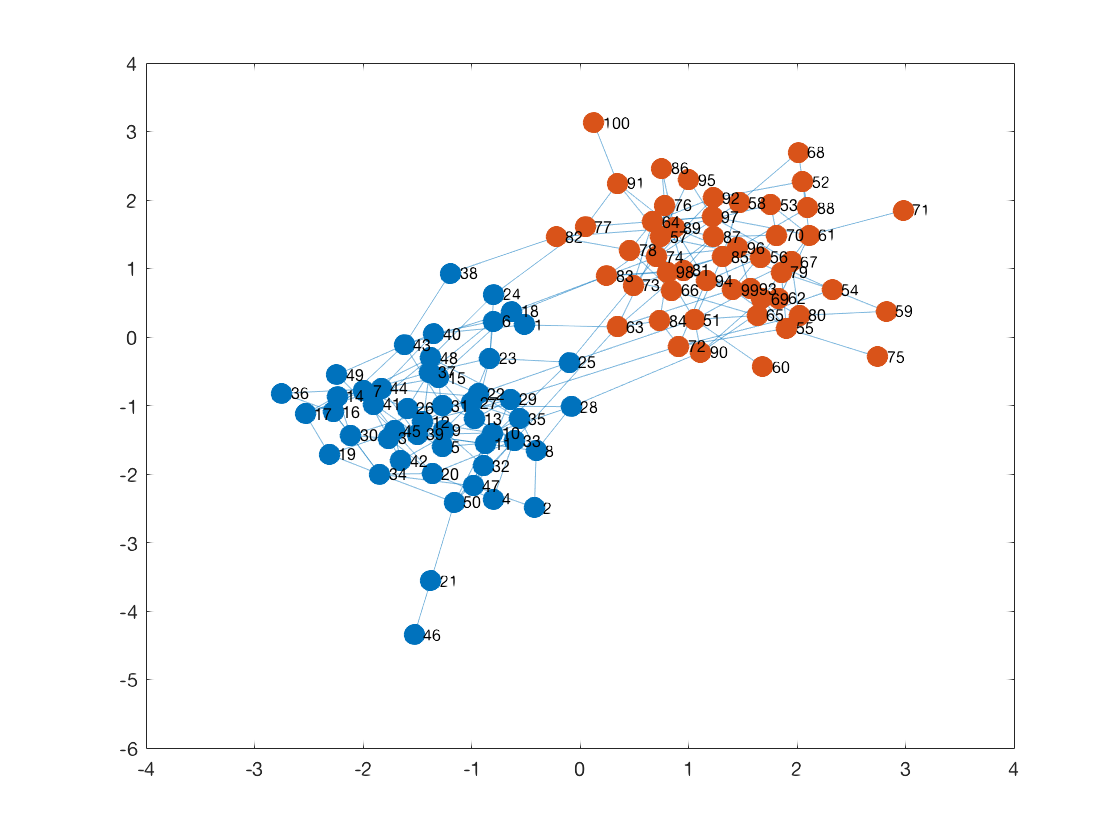
\includegraphics[width=.5\textwidth]{stochasticBlock.png}
		\vspace{-1em}
	\end{center}
	To do so, we need to understand the second smallest eigenvector of $\bv{L} = \bv{D} - \bv{A}$. We will start by considering the \emph{expected value} of these matrices:
	\begin{align*}
		\E[\bv{L}] = \E[\bv{D}] -  \E[\bv{A}].
	\end{align*}
\end{frame}

\begin{frame}
	\frametitle{expected adjacency spectrum}
	Letting $G$ be a stochastic block model graph drawn from $G_n(p,q)$ and $\bv A \in \R^{n \times n}$ be its adjacency matrix. $(\E[\bv A])_{i,j} = p$ for $i,j$ in same group, $(\E[\bv A])_{i,j} = q$ otherwise. 
	\begin{columns}
		\begin{column}{.6\textwidth}
			\begin{center}
				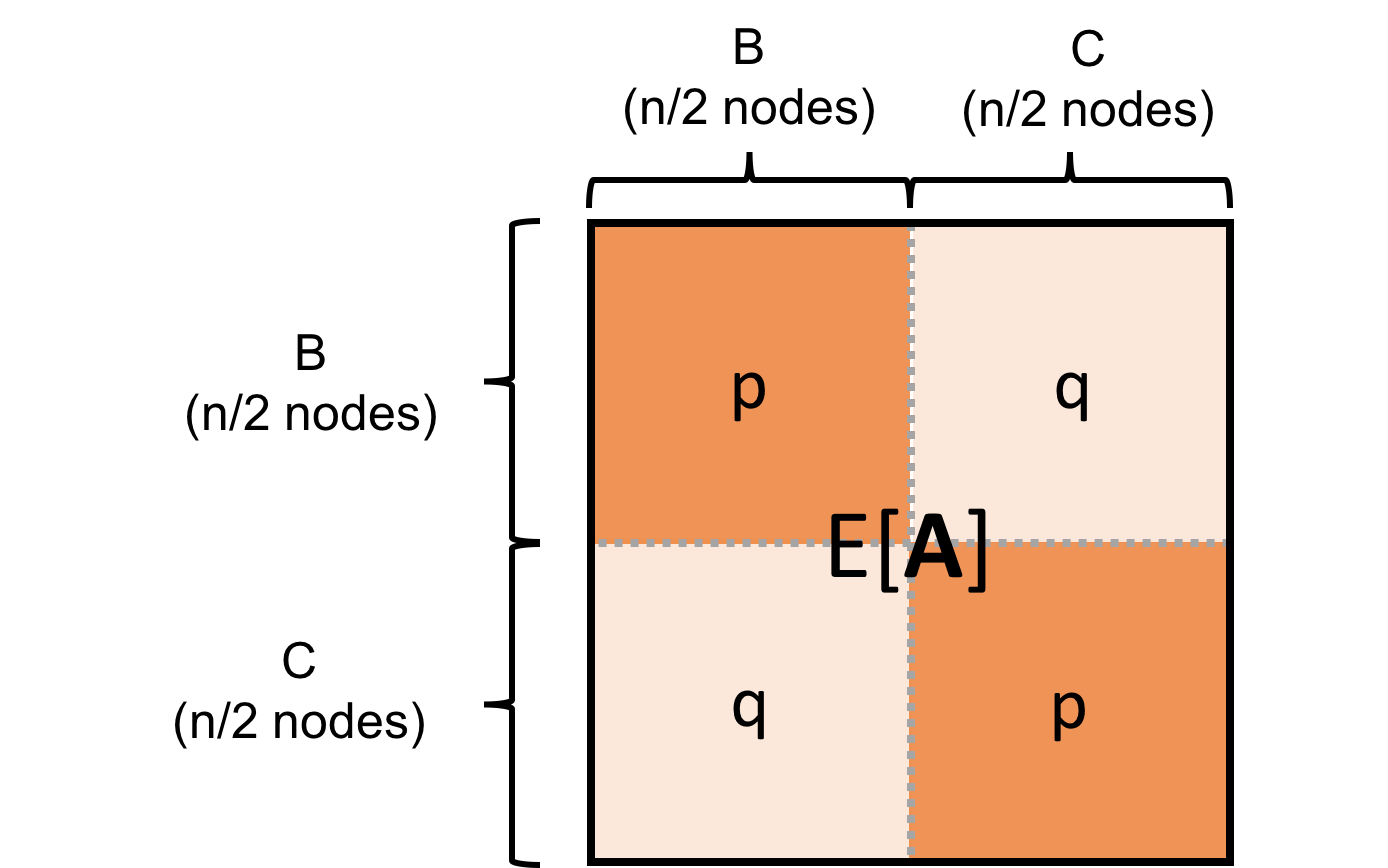
\includegraphics[width=1\textwidth]{expA.png}
			\end{center}
		\end{column}
		\begin{column}{.4\textwidth}
			% We are going to determine the eigenvectors and eigenvalues of $\E[\bv{A}]$.
		\end{column}
	\end{columns}
\end{frame}

\begin{frame}
	\frametitle{expected laplacian}
	\begin{center}
		What is the expected Laplacian of $G_n(p,q)$?
		\vspace{14em}
		
		
		$\E[\bv{A}]$ and $\E[\bv{L}]$ have the same eigenvectors and eigenvalues are equal up to a shift/inversion. So second largest eigenvector of $\E[\bv{A}]$ is the same as the second smallest of $\E[\bv{L}]$
	\end{center}
\end{frame}

\begin{frame}[t]
	\frametitle{expected adjacency spectrum}
	Letting $G$ be a stochastic block model graph drawn from $G_n(p,q)$ and $\bv A \in \R^{n \times n}$ be its adjacency matrix, what are the eigenvectors and eigenvalues of $\E[\bv{A}]$?
	\vspace{1em}
	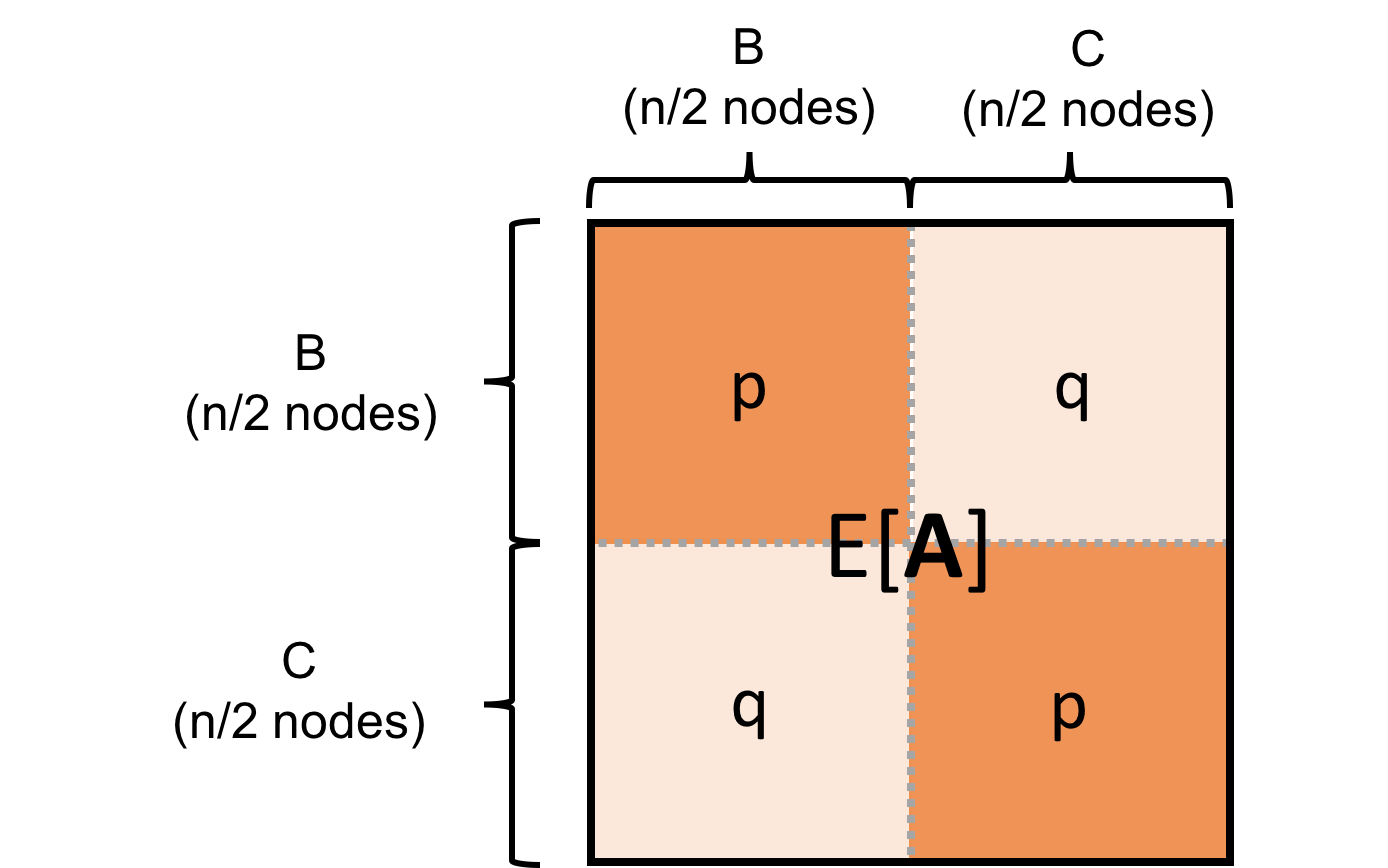
\includegraphics[width=.5\textwidth]{expA.png}
\end{frame}


\begin{frame}
	\frametitle{expected adjacency spectrum}
	\begin{center}
		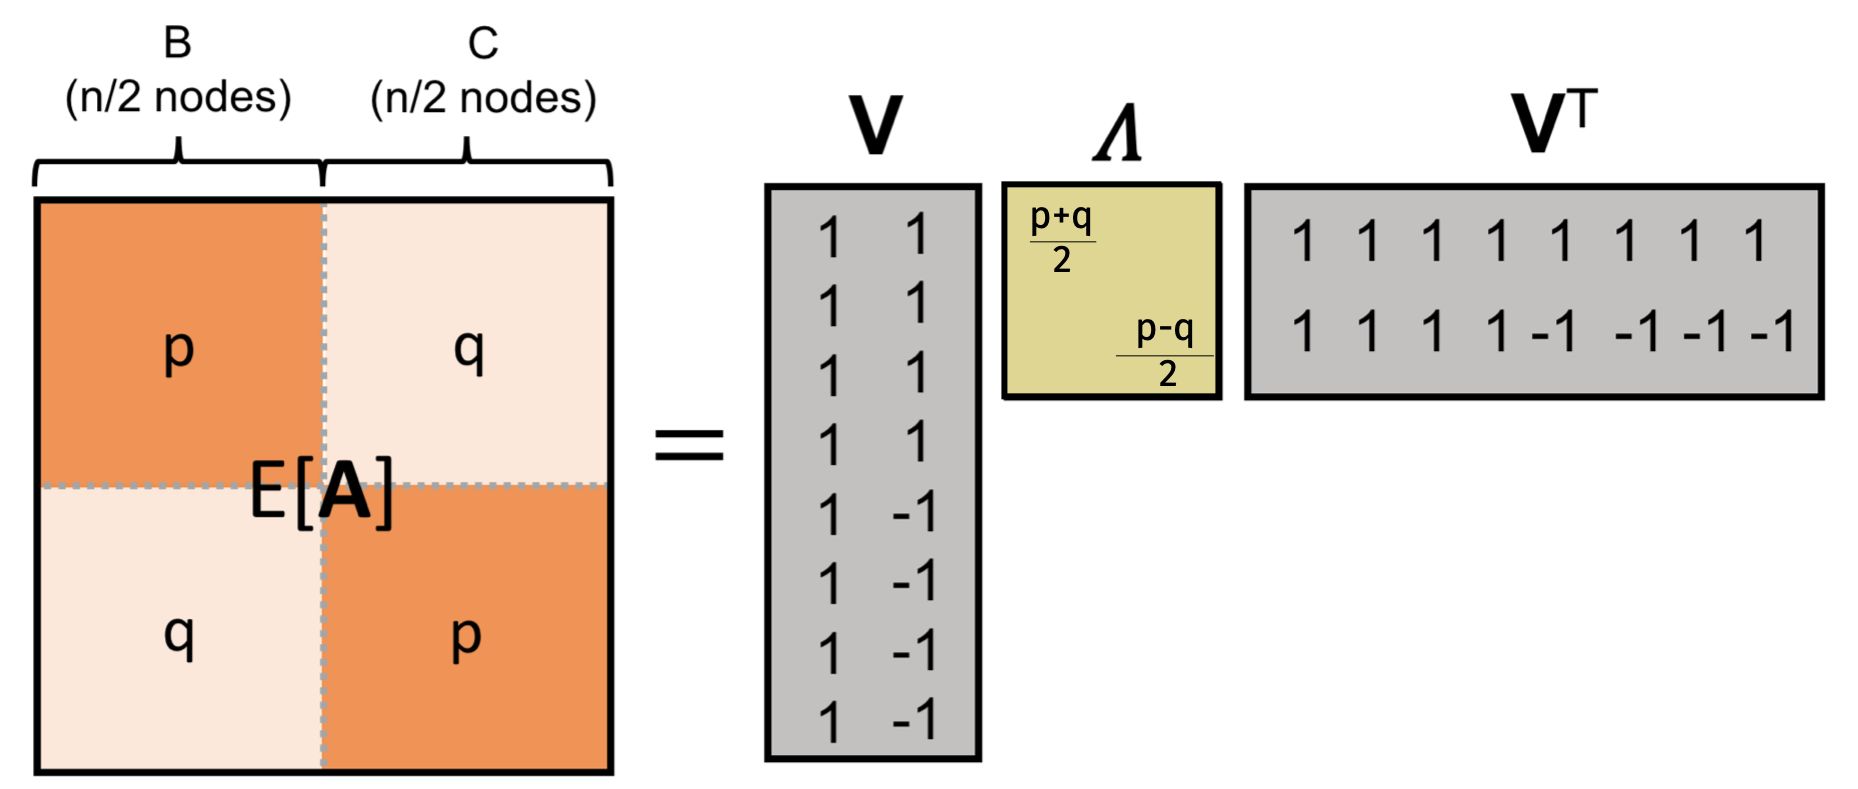
\includegraphics[width=\textwidth]{Aeig_fix.png}
	\end{center}
	\begin{itemize}
		\item $\bar{\bv{v}}_1 \sim \bv{1}$ with eigenvalue $\lambda_1 = \frac{(p+q) n}{2}$.
		\item $\bar{\bv{v}}_2 \sim \bs{\chi}_{B,C}$ with eigenvalue $\lambda_2 = \frac{(p-q) n}{2}$.
	\end{itemize}
	If we compute $\bar{\bv{v}}_2$ then we \emph{exactly recover} the communities $B$ and $C$!
\end{frame}

%\begin{frame}[t]
%	\frametitle{expected laplacian spectrum}
%	Letting $G$ be a stochastic block model graph drawn from $G_n(p,q)$, $\bv A \in \R^{n \times n}$ be its adjacency matrix and $\bv L$ be its Laplacian, what are the eigenvectors and eigenvalues of $\E[\bv{L}]$?
%\end{frame}

\begin{frame}[t]
	\frametitle{expected laplacian spectrum}
	\textbf{Upshot:} The second smallest eigenvector of $\E[\bv{L}]$, equivalently the second largest of $\E[\bv{A}]$, is exactly $\bs{\chi}_{B,C}$ -- the indicator vector for the cut between the communities.
	\begin{itemize}
		\item If the random graph $G$ (equivilantly $\bv{A}$ and $\bv{L}$) were exactly equal to its expectation, partitioning using this eigenvector would exactly recover communities $B$ and $C$.
	\end{itemize}
	\alert{How do we show that a matrix (e.g., $\bv{A}$) is close  to its expectation?} \textbf{Matrix concentration inequalities.}
	\begin{itemize}
		\item Analogous to scalar concentration inequalities like Markovs, Chebyshevs, Bernsteins.
	\end{itemize}
\end{frame}

\begin{frame}
	\frametitle{matrix concentration}
	Alon, Krivelevich, Vu, 2002:
	\begin{tcolorbox}[colback=green!5,colframe=green!40!black]
		\textbf{Matrix Concentration Inequality:}
		If $p \ge O \left ( \frac{\log^4 n}{n} \right )$, then with high probability
		\begin{align*}
		\norm{\bv A - \E[\bv A]}_2 \le O(\sqrt{pn}).
		\end{align*}
		where $\norm{\cdot}_2$ is the matrix \alert{spectral} norm (operator norm).
	\end{tcolorbox}
	Recall that $\norm{\bv{X}}_2 = \max_{z\in\R^d: \norm{z}_2 = 1} \norm{\bv X z}_2 = \sigma_1(\bv{X})$. 
	
	$\|\bv{A}\|_2$ is on the order of $O(p\sqrt{n})$ so another way of thinking about the right hand side is $\frac{\|\bv{A}\|_2}{\sqrt{p}}$. I.e. get's better with $p$.
\end{frame}


\begin{frame}
	\frametitle{eigenvector perturbation}
			For the stochastic block model application, we want to show that the second \emph{eigenvectors} of $\bv{A}$ and $\E[\bv{A}]$ are close. How does this relate to their difference in spectral norm?
	
	\begin{tcolorbox}[colback=green!5,colframe=green!40!black]
		\textbf{Davis-Kahan Eigenvector Perturbation Theorem:}
		Suppose $\bv{A},\bv{\overline A} \in \R^{d \times d}$ are symmetric with $\norm{\bv{A}-\bv{\overline A}}_2 \le \epsilon$ and eigenvectors $\bv{v}_1,\bv{v}_2,\ldots, \bv{v}_n$ and $\bar{\bv{v}}_1,\bar{\bv{v}}_2,\ldots, \bar{\bv{v}}_n$. Letting $\theta(\bv{v}_i,\bar{\bv{v}}_i)$ denote the angle between $\bv{v}_i$ and $\bar{\bv{v}}_i$, for all $i$:
		\begin{align*}
		\sin [\theta(\bv{v}_i, \bar{\bv{v}}_i)] \le \frac{\epsilon}{\min_{j \neq i} |\lambda_i - \lambda_j|}
		\end{align*}
		where $\lambda_1,\ldots,\lambda_n$ are the eigenvalues of $\bv{\overline A}$.
	\end{tcolorbox}
	We will apply with $\bar{\bv{A}} = \E[\bv{A}]$. 
\end{frame}

\begin{frame}
	\frametitle{eigenvector perturbation}
	\begin{center}
		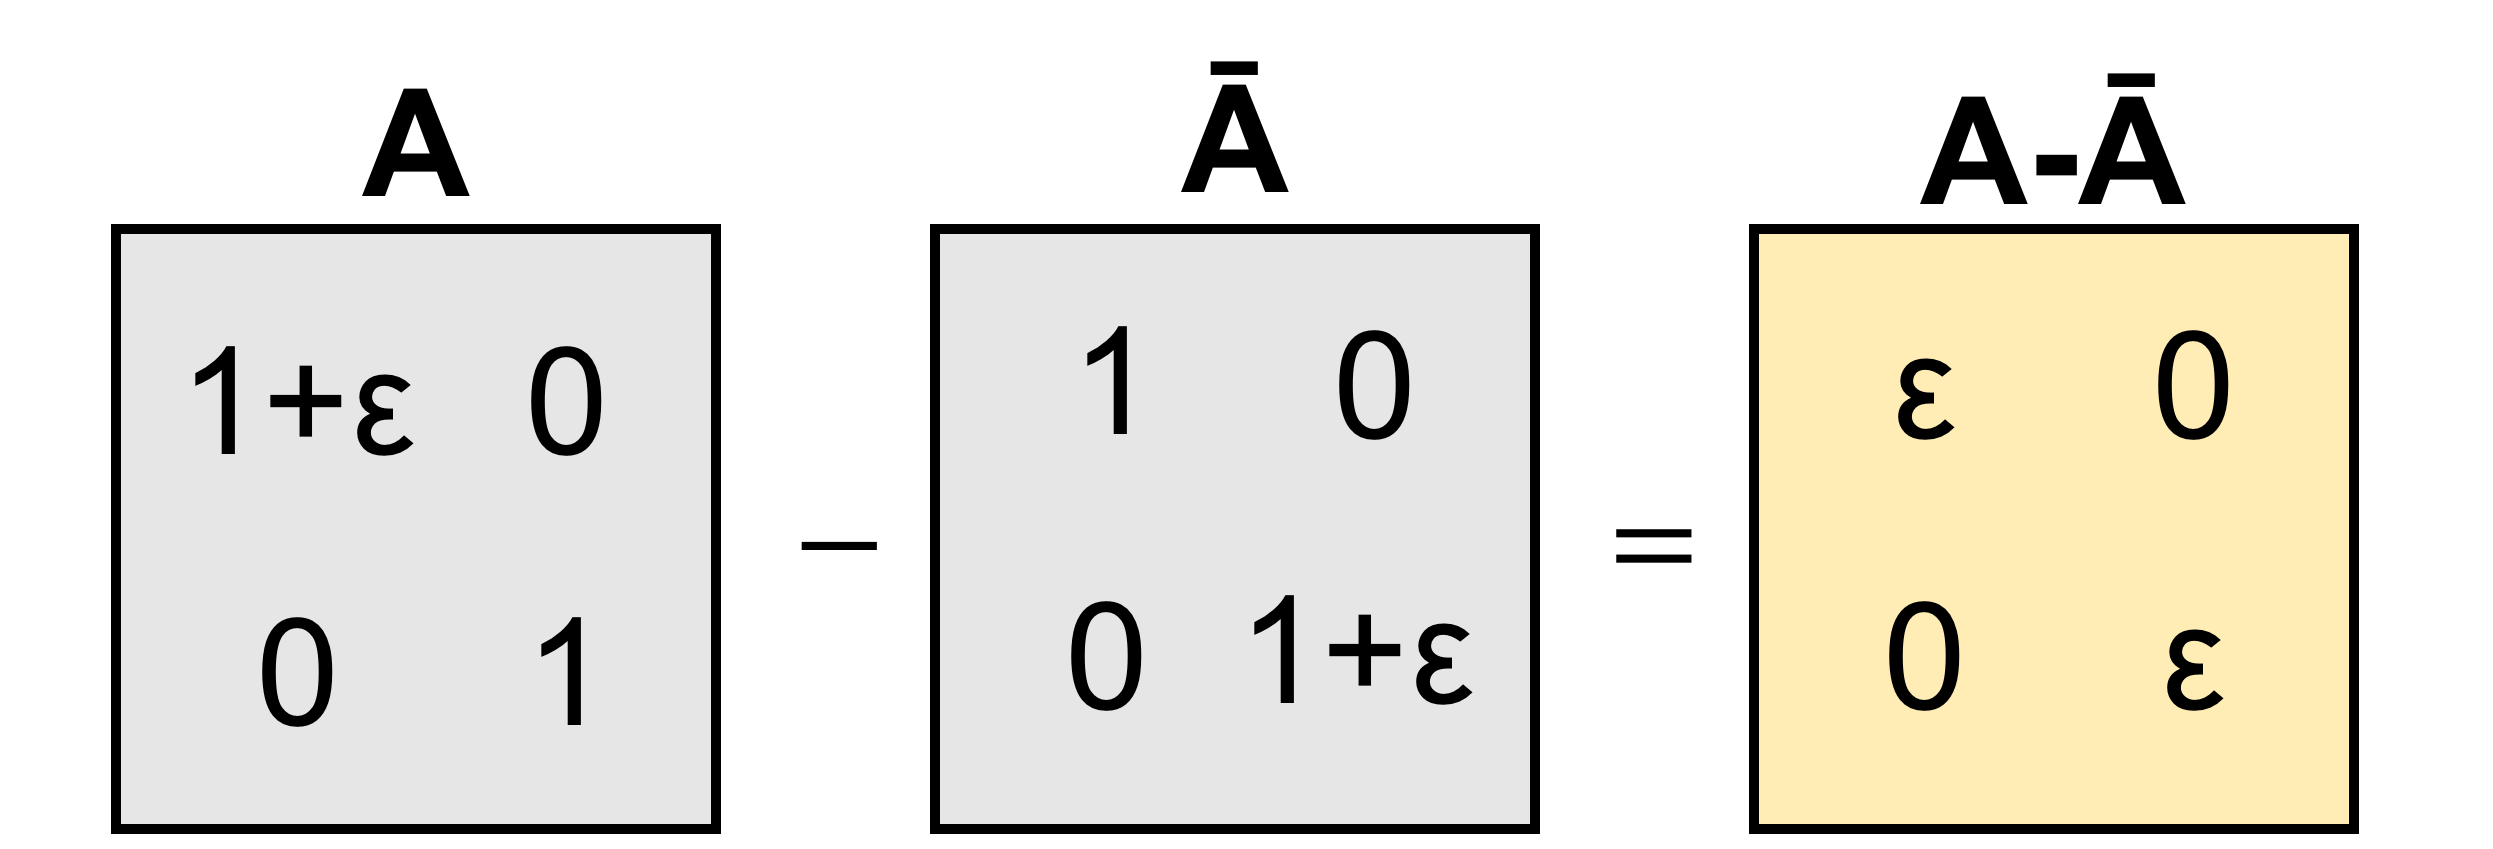
\includegraphics[width=.8\textwidth]{flip.png}
	\end{center}
	\vspace{13em}
\end{frame}

\begin{frame}
	\frametitle{application to stochastic block model}
	%When $\bv{A}$ is the adjacency matrix of a stochastic block model graph with parameters $p$ and $q$:
	%
	\small
	\textbf{Claim 1 (Matrix Concentration):} For $p \ge O\left (\frac{\log^4 n}{n}\right)$, 
	$$\norm{\bv A-\E[\bv{A}]}_2 \le O(\sqrt{pn}).$$

	\begin{tcolorbox}[colback=gray!5,colframe=gray!40!black]
		\textbf{Recall:} $\E[\bv{A}]$, has eigenvalues $\lambda_1 = \frac{(p+q)n}{2}$, $\lambda_2 = \frac{(p-q)n}{2}$, $\lambda_i = 0$ for $i \ge 3$.
			\begin{align*}
			\min_{j \neq i} |\lambda_i - \lambda_j| = \min \left ({qn}, \alert{\frac{(p-q) n}{2}} \right).
			\end{align*}
		Assume $\frac{(p-q) n}{2}$ will be the minimum of these two gaps.
		\end{tcolorbox}
	
	\textbf{Claim 2 (Davis-Kahan):} For $p \ge O\left (\frac{\log^4 n}{n}\right)$, 
	$$\sin \theta(\bv{v}_2,\bar{\bv{v}}_2) \le \frac{O(\sqrt{pn})}{\min_{j \neq i} |\lambda_i - \lambda_j|} \le \frac{O(\sqrt{p n})}{(p-q)n/2} = \alert{O\left (\frac{\sqrt{p}}{(p-q)\sqrt{n}} \right )}
	$$
	
(A slightly trickier analysis can remove the $qn$ term entirely.)
\end{frame}

\begin{frame}
	\frametitle{application to stochastic block model}
	\small
	\textbf{So far:} $\sin \theta(\bv{v}_2,\bar{\bv{v}}_2) \le O\left (\frac{\sqrt{p}}{(p-q)\sqrt{n}} \right )$. What does this give us?
	\begin{itemize}
		\item Can show that this implies $\norm{\bv{v}_2 - \bar{\bv{v}}_2}_2^2 \le O\left (\frac{p}{(p-q)^2 n} \right )$ (exercise).
		\item $\bar{\bv{v}}_2$ is $\frac{1}{\sqrt{n}} \chi_{B,C}$: the community  indicator vector.
		\begin{center}
			\vspace{-1.5em}
			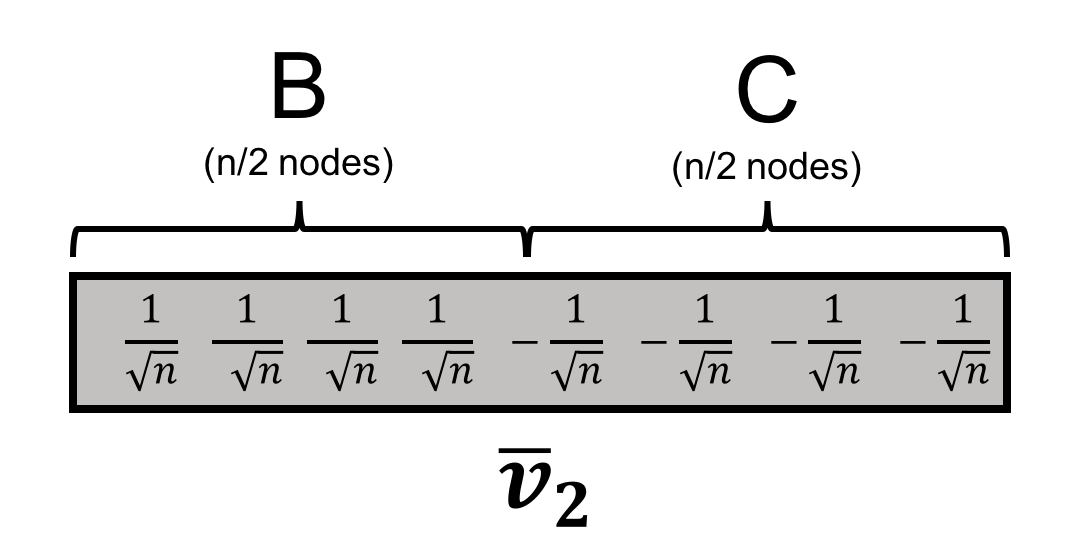
\includegraphics[width=.5\textwidth]{v2.png}
				\vspace{-1em}
		\end{center}
		\item We want to show that $\sign(\bv{v}_2)$ and $\bar{\bv{v}_2}$ are close. They only differ at locations where $\bv{v}_2$ and $\bar{\bv{v}_2}$ differ in sign.
			\begin{center}
			\vspace{-2em}
			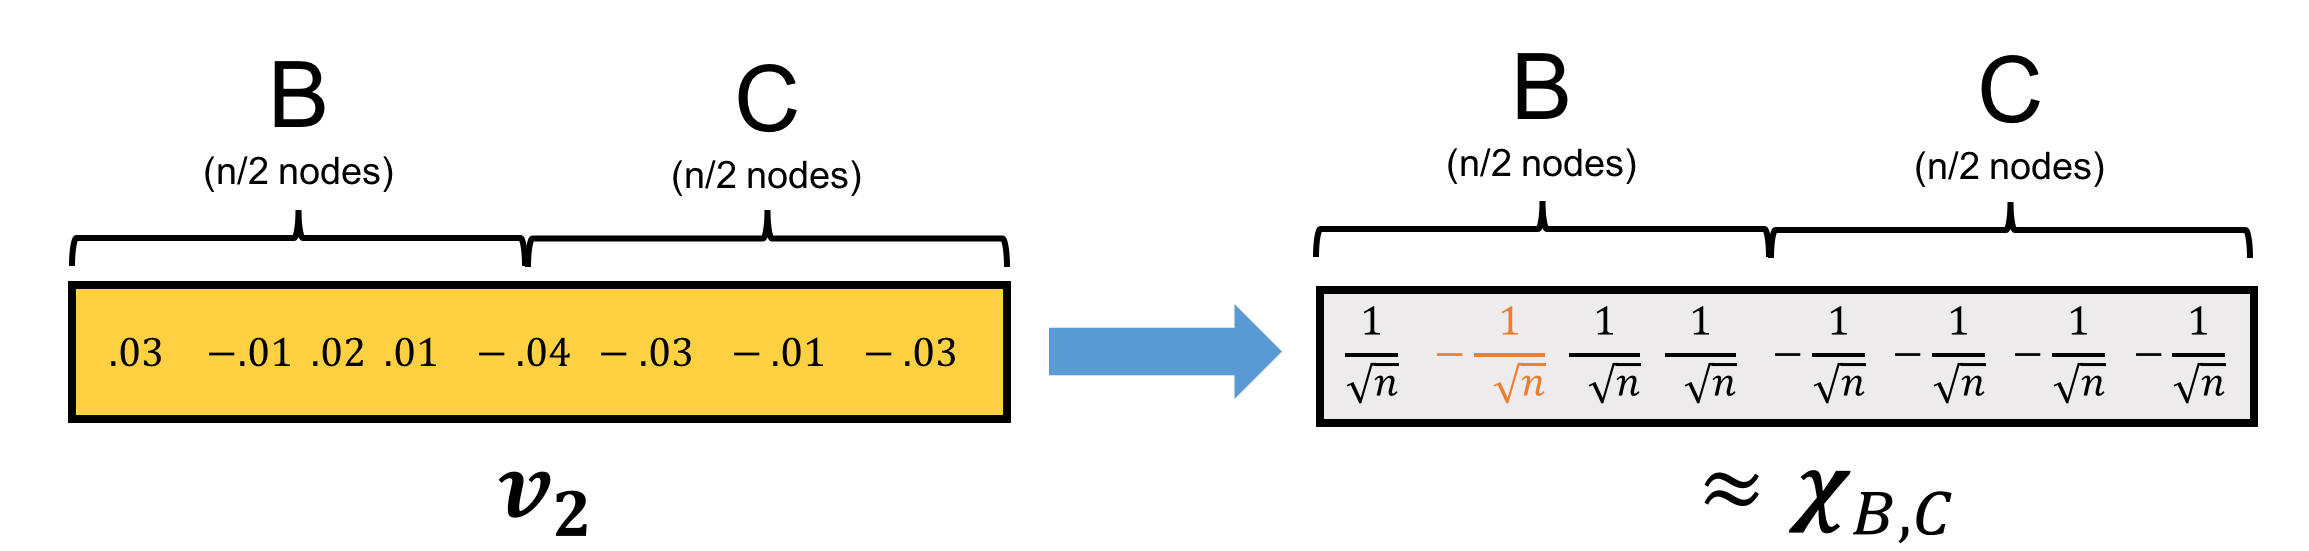
\includegraphics[width=1\textwidth]{round.png}
		\end{center}
	\end{itemize}
\end{frame}

\begin{frame}
	\frametitle{application to stochastic block model}
	\textbf{Main argument:}
	\begin{itemize}
		\item Every $i$ where $v_2(i)$, $\bar v_2(i)$ \alert{differ in sign} contributes $\ge \frac{1}{n}$ to $\norm{\bv{v}_2 - \bar{\bv{v}}_2}_2^2.$
		\item We know that $\norm{\bv{v}_2 - \bar{\bv{v}}_2}_2^2 \le O\left (\frac{p}{(p-q)^2 n} \right )$.
		\item So $\bv{v}_2$ and $\bar{\bv{v}}_2$ differ in sign in at most $O \left  (\frac{p}{(p-q)^2}\right )$ positions.	\end{itemize}
\end{frame}




%\begin{frame}
%\frametitle{Matrix Concentration}
%In scalar concentration bounds we measure distance by the magnitude $|\bv{x} - \E[\bv x]|$. \alert{How should we measure distance in matrix concentration bounds?}
%\begin{itemize}
%\item In our stochastic block model application, letting $\hat v_2$ and $v_2$ be the second largest eigenvectors of $\bv{A}$ and $\E[\bv{A}]$ respectively, we want: 
%\end{itemize}
%\end{frame}

\begin{frame}
	\frametitle{application to stochastic block model}
	\textbf{Upshot:} If $G$ is a stochastic block model graph with adjacency matrix $\bv{A}$, if we compute its second largest eigenvector $\bv{v}_2$ and assign nodes to communities according to the sign pattern of this vector, we will correctly assign all but $O \left  (\frac{p}{(p-q)^2} \right  )$ nodes.
	\begin{itemize}
		\item \textbf{Hard case:} Suppose $q = .8  p$ so $\frac{p}{(p-q)^2} = 25/p$. Even if $p$ is really small, i.e. $p = 250/n$, then we assign roughly $90\%$ of nodes to the right partition.
	\end{itemize}
\end{frame}

\begin{frame}[t]
	\frametitle{randomized numerical linear algebra}
	Forget about the previous problem, but still consider the matrix $\bv{M} = \E[\bv{A}]$.
	\begin{itemize}
		\item Dense $n \times n$ matrix.
		\item Computing top eigenvectors takes $\approx O(n^2 / \sqrt{\epsilon})$ time.
	\end{itemize}
	If someone asked you to speed this up and return \emph{approximate} top eigenvectors, what could you do?
\end{frame}

\begin{frame}
	\frametitle{randomized numerical linear algebra}
	\textbf{Main idea:}
	If you want to compute singular vectors, multiply two matrices, solve a regression problem, etc.:
	\begin{enumerate}
		\item Compress your matrices using a randomized method (e.g. subsampling).
		\item Solve the problem on the smaller or sparser matrix.
		\begin{itemize}
			\item $\bv{\~{A}}$ called a ``sketch'' or ``coreset'' for $\bv{A}$. 
		\end{itemize}
	\end{enumerate}

\begin{center}
	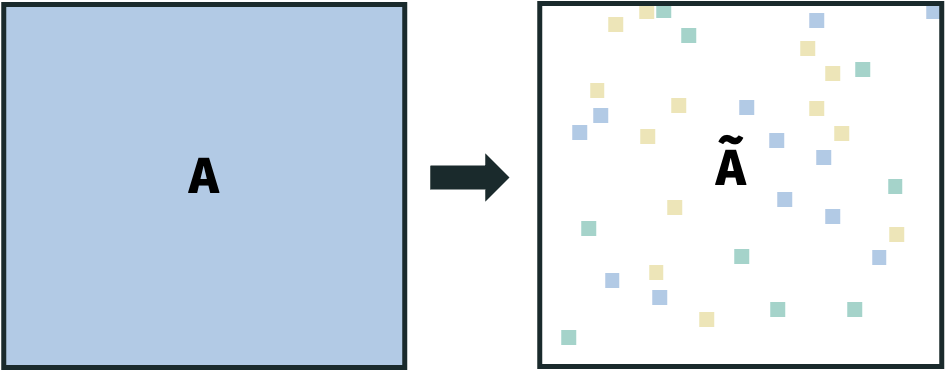
\includegraphics[height=.25\textheight]{entrywisesample.png}\hfill
	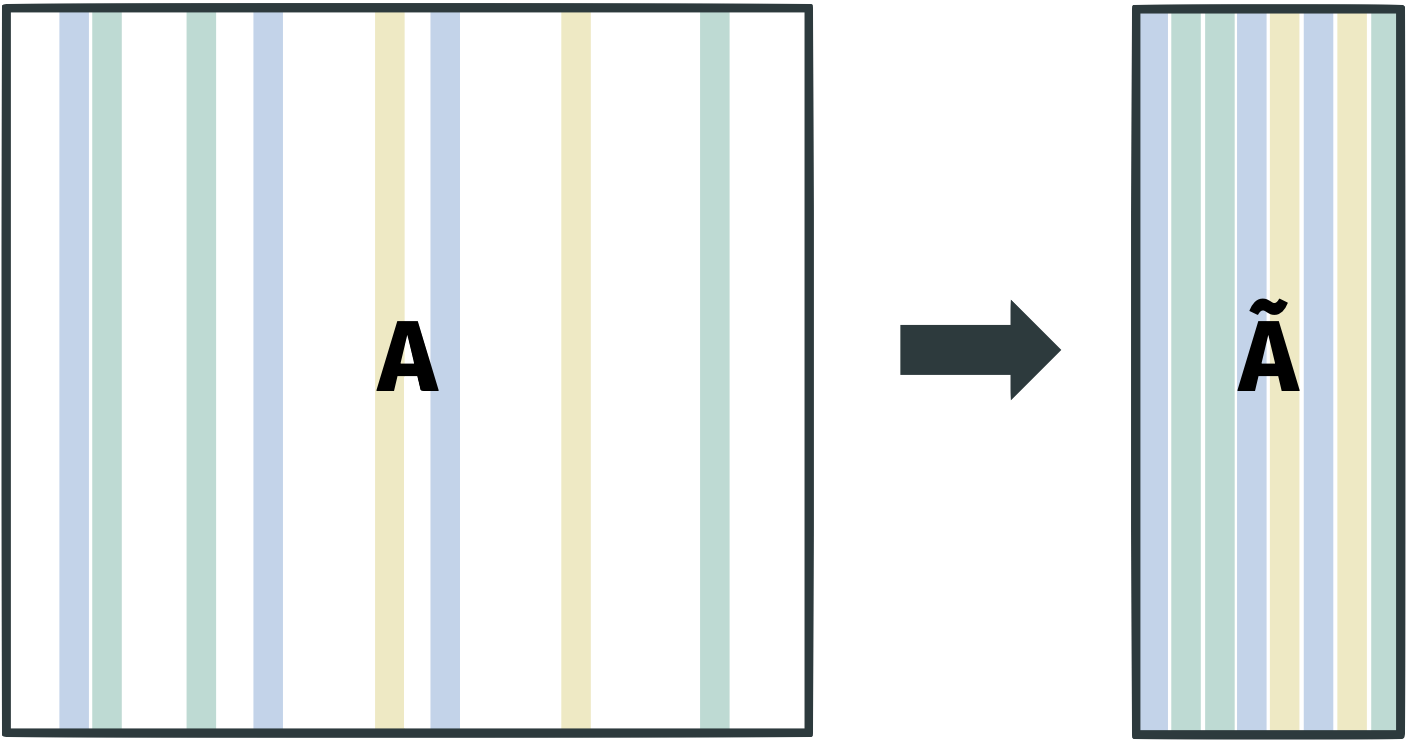
\includegraphics[height=.25\textheight]{sampling_column_reduction.png}
	\medskip
	
	 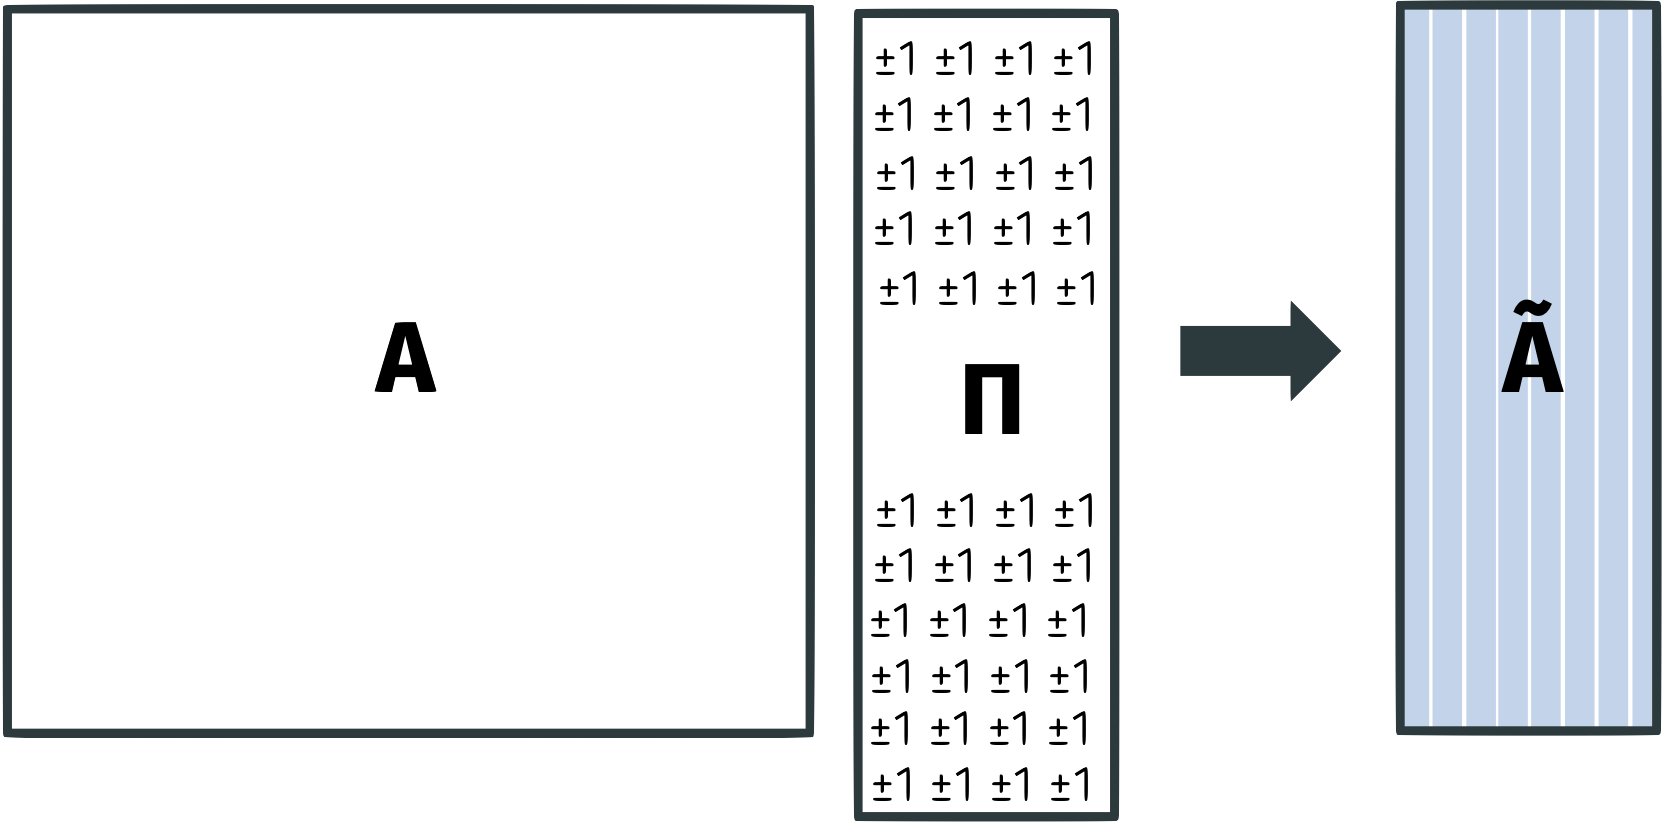
\includegraphics[height=.25\textheight]{projection_column_reduction1.png}\hfill
	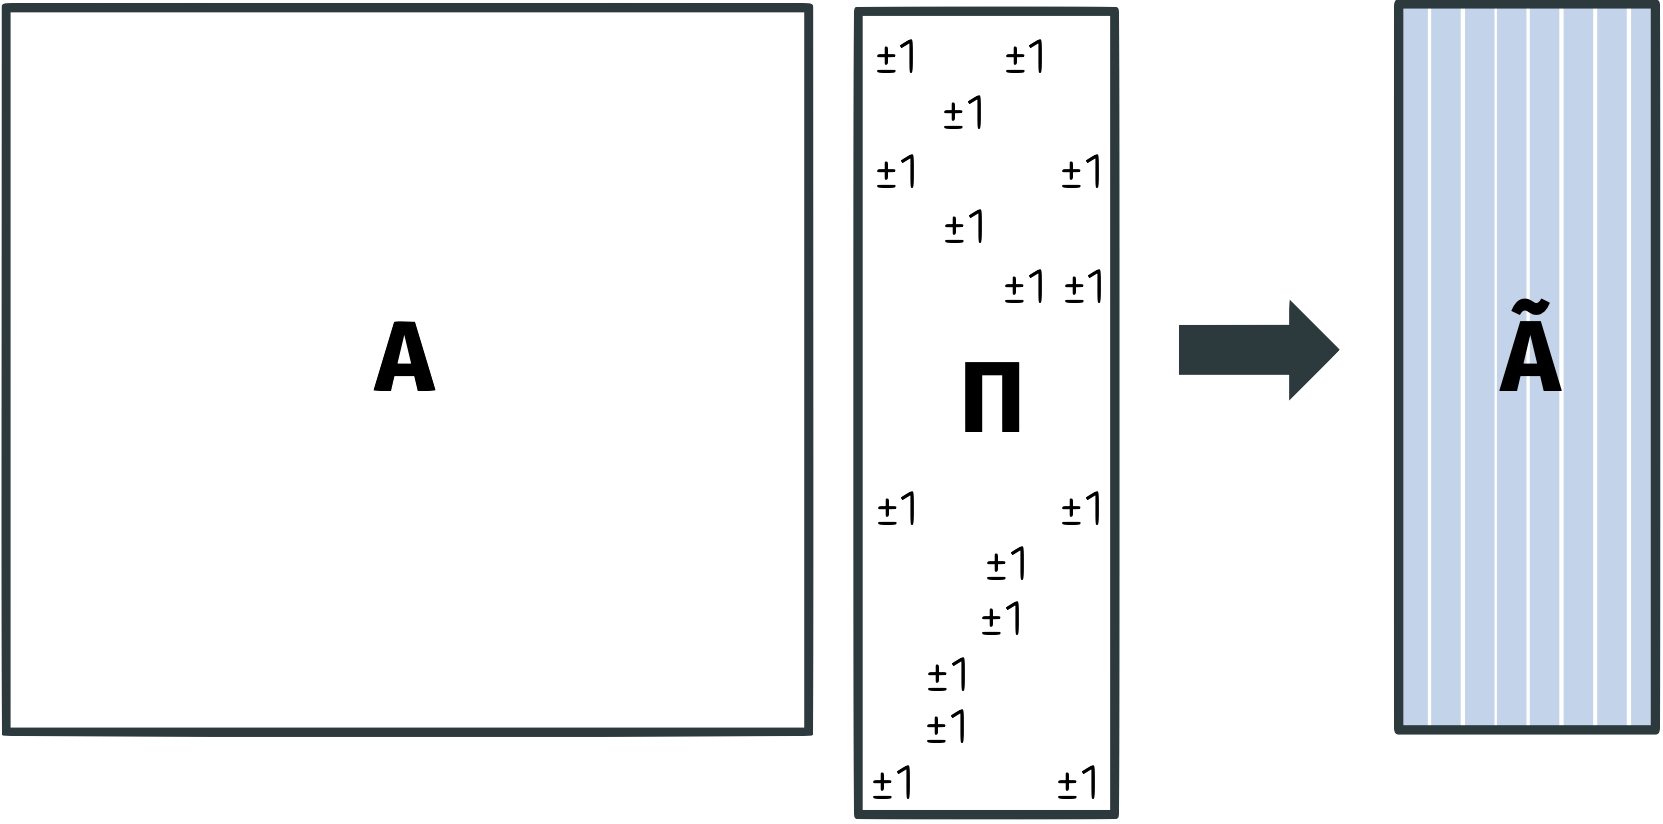
\includegraphics[height=.25\textheight]{projection_column_reduction2.png}
\end{center}
\end{frame}

\begin{frame}[standout]
	\begin{center}
			\large break
		\end{center}
\end{frame}

\begin{frame}[t]
	\frametitle{randomized numerical linear algebra}
	\textbf{Approximate matrix multiplication:}
	\begin{center}
		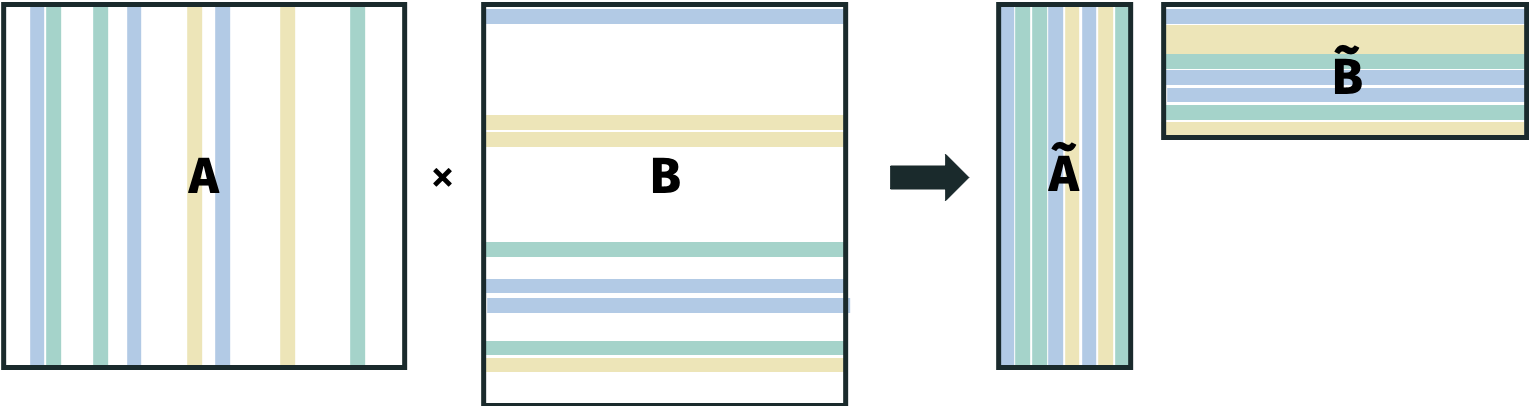
\includegraphics[width=.9\textwidth]{matrix_mult.png}
	\end{center}
	\textbf{Approximate regression:}
	\begin{center}
		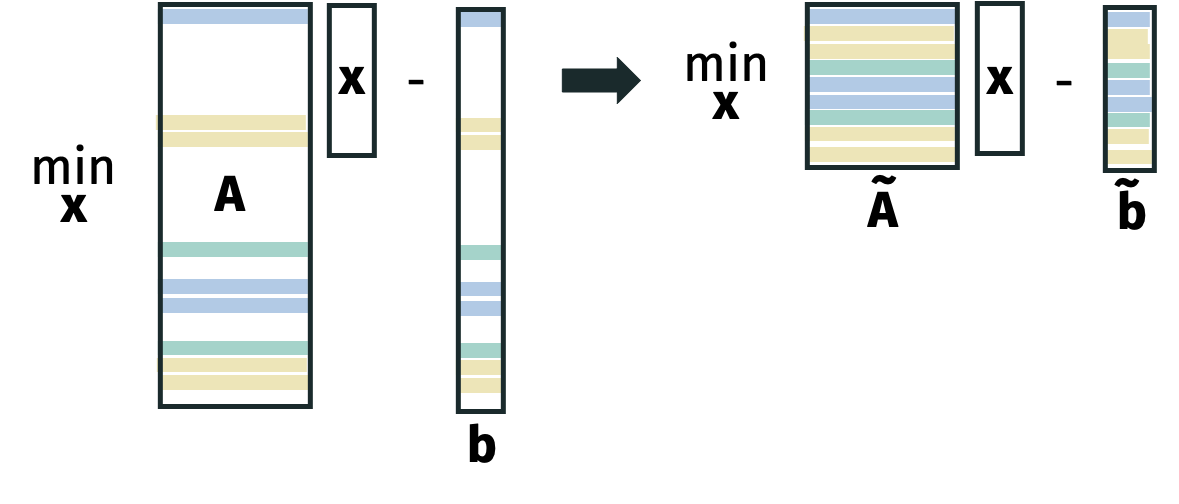
\includegraphics[width=.7\textwidth]{subsampledRegressioon.png}
	\end{center}
\end{frame}



\begin{frame}[t]
	\frametitle{sketched regression}
	\textbf{Today's example:} Randomized approximate regression using a Johnson-Lindenstrauss matrix for compression.
	\begin{center}
		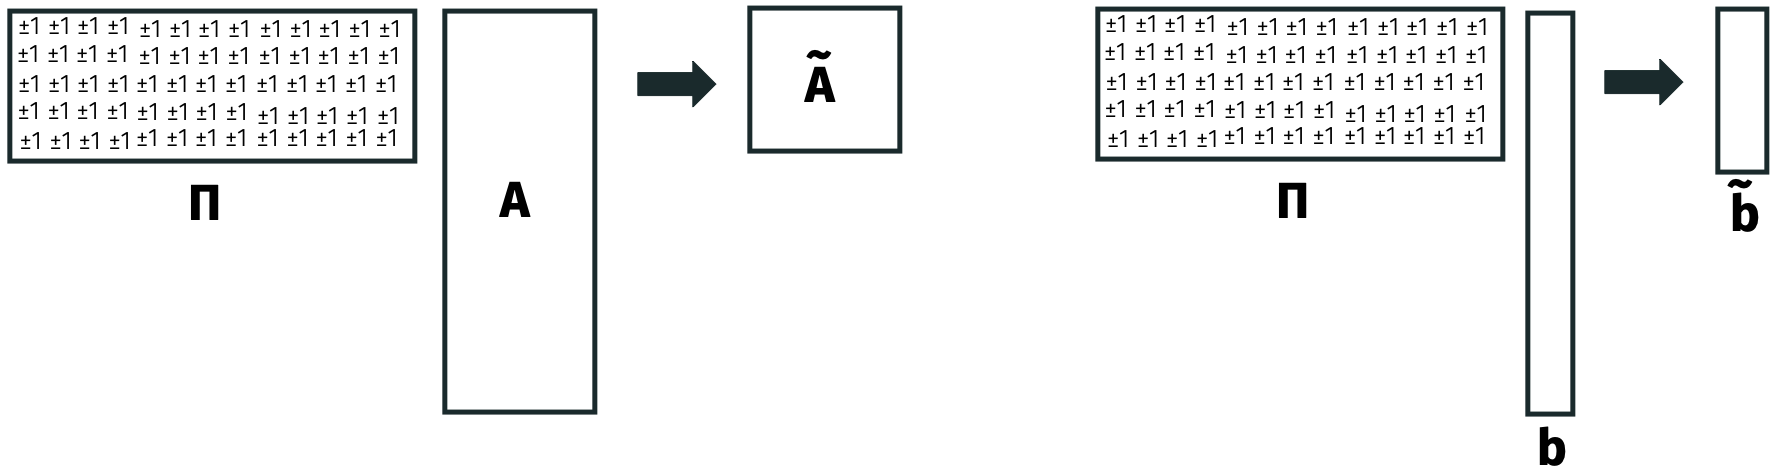
\includegraphics[width=\textwidth]{jlRegression.png}
	\end{center}
		\vspace{-.5em}

	\textbf{Input}: $\bv{A} \in \R^{n\times d}$, $\bv{b} \in \R^{n}$. 
	
	\textbf{Goal}: Let $\bv{x}^* = \argmin_{\bv{x}}\|\bv{A}\bv{x} - \bv{b}\|_2^2$. Let $\tilde{\bv{x}} = \argmin_{\bv{x}}\|\bs{\Pi}{\bv{A}}\bv{x} - \bs{\Pi}\tilde{\bv{b}}\|_2^2$
	
\vspace{-2em}
	\begin{center}	
	\begin{align*}
		\text{Want: }\|\bv{A}\tilde{\bv{x}} - \bv{b}\|_2^2 \leq \left(1+\epsilon\right) \|\bv{A}\bv{x}^* - \bv{b}\|_2^2
 	\end{align*}

%	\alert{If $\bs{\Pi} \in \R^{m\times n}$, how large does $m$ need to be? Is it even clear this should work as $m \rightarrow \infty$?}
\end{center}
\end{frame}

\begin{frame}[t]
\frametitle{target result}
\begin{theorem}[Randomized Linear Regression]
	Let $\bs{\Pi}$ be a properly scaled JL matrix (random Gaussian, sign, sparse random, etc.) with $m = O\left(\frac{d}{\epsilon^2}\right)$ rows\footnote{This can be improved to $O(d/\epsilon)$ with a tighter analysis}. Then with probability $9/10$, for any $\bv{A}\in \R^{n\times d}$ and $\bv{b}\in \R^n$,
	\begin{align*}
		\|\bv{A}\tilde{\bv{x}} - \bv{b}\|_2^2 \leq (1+\epsilon) \|\bv{A}\bv{x}^* - \bv{b}\|_2^2
	\end{align*}
	where $\tilde{\bv{x}} = \argmin_{\bv{x}} \|\bs{\Pi}\bv{A}\bv{x} - \bs{\Pi}\bv{b}\|_2^2$.
\end{theorem}
\end{frame}

\begin{frame}
	\frametitle{plan}
	\begin{itemize}
	\item Prove this theorem using an \emph{$\epsilon$-net argument}, which is a popular technique for applying our standard concentration inequality + union bound argument to an \emph{infinite number of events}.
	
	\item These sort of arguments appear all the time in theoretical algorithms and ML research, so this part of lecture is as much about the technique as the final result. 
	
	\item For the bonus problem on your last problem set you will use an $\epsilon$-net argument to prove a matrix concentration inequality on your last problem set. 
	\end{itemize}
\end{frame}

\begin{frame}[t]
	\frametitle{sketched regression}
	\textbf{Claim}: Suffices to prove that \emph{for all $\bv{x} \in \R^d$},
	\begin{align*}
		(1-\epsilon)\|\bv{A}\bv{x} - \bv{b}\|_2^2 \leq  \|\bs{\Pi}\bv{A}\bv{x} - \bs{\Pi}\bv{b}\|_2^2 \leq (1+\epsilon) \|\bv{A}\bv{x} - \bv{b}\|_2^2
	\end{align*}
\end{frame}

\begin{frame}[t]
	\frametitle{distributional johnson-lindenstrauss review}
	\begin{lemma}[Distributional JL]
		If $\bs{\Pi}$ is chosen to a properly scaled random Gaussian matrix, sign matrix, sparse random matrix, etc., with $O\left(\frac{\log(1/\delta}{\epsilon^2}\right)$ rows then \emph{for any fixed $\bv{y}$}, 
		\begin{align*}
			(1-\epsilon)\|\bv{y}\|_2^2 \leq  \|\bs{\Pi}\bv{y}\|_2^2 \leq (1+\epsilon) \|\bv{y}\|_2^2
		\end{align*}
		with probability $(1-\delta)$. 
	\end{lemma}

\vspace{2em}
\textbf{Corollary:} \emph{For any fixed $\bv{x}$}, with probability $(1-\delta)$,
		\begin{align*}
(1-\epsilon)\|\bv{A}\bv{x} - \bv{b}\|_2^2 \leq  \|\bs{\Pi}\bv{A}\bv{x} - \bs{\Pi}\bv{b}\|_2^2 \leq (1+\epsilon) \|\bv{A}\bv{x} - \bv{b}\|_2^2.
\end{align*}
	
\end{frame}

\begin{frame}[t]
	\frametitle{for any to for all}
	\begin{center}
	How do we go from ``\emph{for any fixed $\bv{x}$}'' to ``\emph{for all $\bv{x} \in \R^d$}''.
	\end{center}
	
	This statement requires establishing a Johnson-Lindenstrauss type bound for an \emph{infinity} of possible vectors $(\bv{A}\bv{x} - \bv{b})$, which can't be tackled directly with a union bound argument. 
	\vspace{4em}
	
	Note that all vectors of the form  $(\bv{A}\bv{x} - \bv{b})$ lie in a low dimensional subspace: spanned by $d+1$ vectors, where $d$ is the width of $\bv{A}$. \alert{\textbf{So even though the set is infinite, it is ``simple'' in some way. Parameterized by just $d + 1$ numbers.}}
\end{frame}


\begin{frame}
	\frametitle{subspace embeddings}
	\begin{theorem}[Subspace Embedding from JL]
		Let $\mathcal{U} \subset \R^n$ be a $d$-dimensional linear subspace in $\R^n$. If $\bs{\Pi}\in \R^{m\times d}$ is chosen from any distribution $\mathcal{D}$ satisfying the Distributional  JL Lemma, then with probability $1-\delta$,
		\begin{align*}
			(1-\epsilon)\|\bv{v}\|_2^2 \leq \|\Pi \bv{v}\|_2^2 \leq	(1+\epsilon)\|\bv{v}\|_2^2
		\end{align*}
		for \emph{all} $\bv{v} \in \mathcal{U}$, as long as  $m = O\left(\frac{d\log(1/\epsilon) + \log(1/\delta)}{\epsilon^2}\right)$.\footnote{It's possible to obtain a slightly tighter bound of $O\left(\frac{d+\log(1/\delta)}{\epsilon^2}\right)$. It's a nice challenge to try proving this.}
		%	I.e. for some matrix $S\in \R^{d\times s}$, $\mathcal{U}$ contains all vectors $v$ that can be written $v = Sx$ for some $x \in \R^q$.
	\end{theorem}
	\begin{center}
		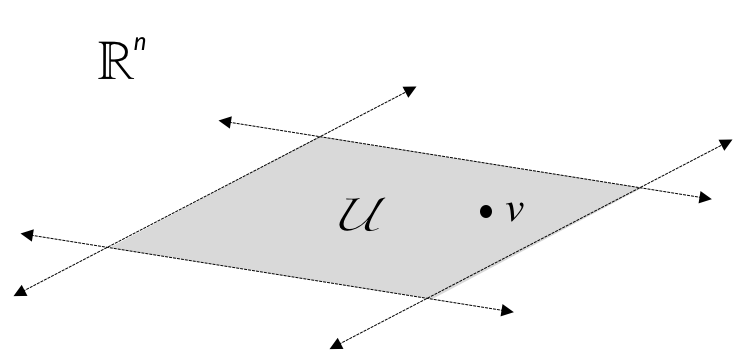
\includegraphics[width=0.4\textwidth]{subspace_vis.png}
	\end{center}
\end{frame}

\begin{frame}
	\frametitle{subspace embedding to approximate regression}
	\textbf{Corollary:} If we choose $\bs{\Pi}$ and properly scale, then with $O\left(d/\epsilon^2\right)$ rows, 
	\begin{align*}
		(1-\epsilon)\|\bv{A}\bv{x} - \bv{b}\|_2^2 \leq  \|\bs{\Pi}\bv{A}\bv{x} - \bs{\Pi}\bv{b}\|_2^2 \leq (1+\epsilon) \|\bv{A}\bv{x} - \bv{b}\|_2^2
	\end{align*}
	\emph{for all $\bv{x}$} and thus
	\begin{align*}
		\|\bv{A}\tilde{\bv{x}} - \bv{b}\|_2^2 \leq \left(1+O(\epsilon)\right) \min_{\bv{x}} \|\bv{A}\bv{x} - \bv{b}\|_2^2.
	\end{align*} 
	\begin{center}
		\alert{\textbf{I.e., our main theorem is proven.}}
	\end{center}
	
	\textbf{Proof:} Apply Subspace Embedding Thm. to the $(d+1)$ dimensional subspace spanned by $\bv{A}$'s $d$ columns and $\bv{b}$. Every vector $\bv{Ax - b}$ lies in this subspace.
\end{frame}

\begin{frame}
	\frametitle{subspace embeddings}
	\begin{theorem}[Subspace Embedding from JL]
		Let $\mathcal{U} \subset \R^n$ be a $d$-dimensional linear subspace in $\R^n$. If $\bs{\Pi}\in \R^{m\times d}$ is chosen from any distribution $\mathcal{D}$ satisfying the Distributional JL Lemma, then with probability $1-\delta$,
		\begin{align}
			\label{se_goal}
			(1-\epsilon) \|\bv{v}\|_2^2 \leq \|\Pi \bv{v}\|_2^2 \leq	(1+\epsilon)\|\bv{v}\|_2^2
		\end{align}
		for \emph{all} $\bv{v} \in \mathcal{U}$, as long as  $m = O\left(\frac{d\log(1/\epsilon) + \log(1/\delta)}{\epsilon^2}\right)$
	\end{theorem}
	\begin{center}
		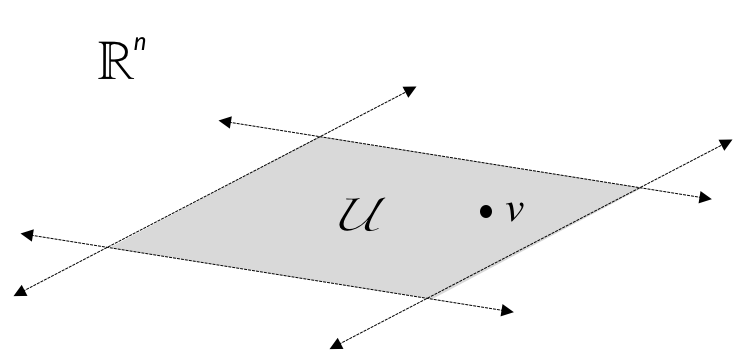
\includegraphics[width=0.4\textwidth]{subspace_vis.png}
		
		\textbf{\alert{Subspace embeddings have tons of other applications!}}
	\end{center}
\end{frame}

\begin{frame}
	\frametitle{subspace embedding proof}
	\begin{align}
		(1-\epsilon) \|\bv{v}\|_2^2 \leq \|\Pi \bv{v}\|_2^2 \leq	(1+\epsilon)\|\bv{v}\|_2^2
	\end{align}

	\textbf{First Observation:}
	The theorem holds as long as \eqref{se_goal} holds for all $\bv{w}$ on the unit sphere in $\mathcal{U}$. Denote the sphere $S_{\mathcal{U}}$:
	\begin{align*}
		S_{\mathcal{U}} = \{\bv{w} \,|\, \bv{w}\in \mathcal{U} \text{ and } \|\bv{w}\|_2 = 1 \}. 
	\end{align*}
	\textbf{Follows from linearity:} Any point $\bv{v} \in \mathcal{U}$ can be written as $c \bv{w}$ for some scalar $c$ and some point $\bv{w} \in S_{\mathcal{U}}$. 
	\begin{center}
		\begin{itemize}
			\item If $(1-\epsilon)\|\bv{w}\|_2 \leq \|\bs{\Pi} \bv{w}\|_2 \leq	(1+\epsilon)\|\bv{w}\|_2$. 
			\item then ${c}(1-\epsilon)\|\bv{w}\|_2 \leq {c}\|\bs{\Pi} \bv{w}\|_2 \leq	{c}(1+\epsilon)\|\bv{w}\|_2$,
			\item and thus $(1-\epsilon)\|c\bv{w}\|_2 \leq \|\bs{\Pi} c\bv{w}\|_2 \leq	(1+\epsilon)\|c\bv{w}\|_2$.
		\end{itemize}  
	\end{center}
\end{frame}


\begin{frame}
	\frametitle{subspace embedding proof}
	\textbf{Intuition:} There are not too many ``different'' points on a $d$-dimensional sphere:
	\vspace{-1em}
	\begin{center}
		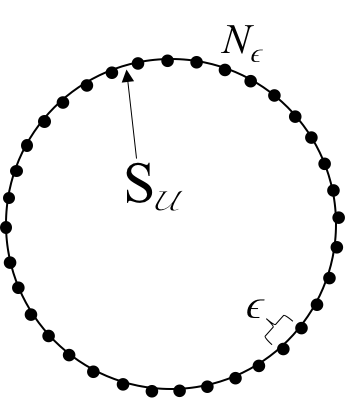
\includegraphics[width=0.3\textwidth]{2dnet.png}
	\end{center}
	$N_\epsilon$ is called an ``$\epsilon$''-net.
	
	If we can prove
	\begin{align*}
		(1-\epsilon)\|\bv{w}\|_2 \leq \|\Pi \bv{w}\|_2 \leq	(1+\epsilon)\|\bv{w}\|_2
	\end{align*} 
	for all points $\bv{w} \in N_\epsilon$, we can hopefully extend to all of $S_{\mathcal{U}}$. 
\end{frame}

\begin{frame}[t]
	\frametitle{$\epsilon$-net for the sphere}
	\begin{lemma}[$\epsilon$-net for the sphere]
		For any $\epsilon \leq 1$, there exists a set $N_{\epsilon} \subset S_{\mathcal{U}}$ with $| N_\epsilon | = \left(\frac{4}{\epsilon}\right)^d$ such that $\forall \bv{v} \in S_{\mathcal{U}}$,
		\begin{align*}
			\min_{\bv{w} \in N_\epsilon} \|\bv{v} - \bv{w}\|_2 \leq \epsilon. 
		\end{align*}
	\end{lemma} 
\begin{center}
	\textbf{Take this claim to be true for now: we will prove later.}
\end{center}
\end{frame}

\begin{frame}[t]
	\frametitle{subspace embedding proof}
	\begin{center}
		\alert{\textbf{1. Preserving norms of all points in net $N_\epsilon$.}}
	\end{center}
	
	Set $\delta' = \frac{1}{|\mathcal{N}_{\epsilon}|}\cdot \delta =  \left(\frac{\epsilon}{4}\right)^d\cdot\delta$. As long as $\Pi$ has $O\left(\frac{\log(1/\delta')}{\epsilon^2}\right)$ $= O\left(\frac{d\log(1/\epsilon) + \log(1/\delta)}{\epsilon^2}\right)$ rows, then by a union bound,
	\begin{align*}
		(1-\epsilon)\|\bv{w}\|_2 \leq \|\Pi \bv{w}\|_2 \leq	(1+\epsilon)\|\bv{w}\|_2.
	\end{align*}
for \emph{all} $\bv{w} \in N_\epsilon$ ,with probability $1-\delta$.
\end{frame}

\begin{frame}[t]
	\frametitle{subspace embedding proof}
	\begin{center}
		\alert{\textbf{2. Extending to all points in the sphere.}}
	\end{center}
	For some $\bv{w}_0, \bv{w}_1, \bv{w}_2 \ldots \in N_\epsilon$, any $\bv{v} \in S_{\mathcal{U}}$.  can be written:
	\begin{align*}
		\bv{v} = \bv{w}_0 + c_1\bv{w}_1+ c_2\bv{w}_2 + \ldots
	\end{align*}
	for constants $c_1, c_2,\ldots$ where $|c_i| \leq \epsilon^i$. 
	
	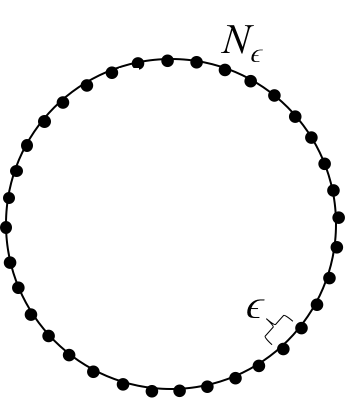
\includegraphics[width=0.3\textwidth]{2dnet_plain.png}
\end{frame}

\begin{frame}[t]
	\frametitle{subspace embedding proof}
	\begin{center}
		\alert{\textbf{2. Extending to all points in the sphere.}}
	\end{center}
	For some $\bv{w}_0, \bv{w}_1, \bv{w}_2 \ldots \in N_\epsilon$, any $\bv{v} \in S_{\mathcal{U}}$.  can be written:
	\begin{align*}
		\bv{v} = \bv{w}_0 + c_1\bv{w}_1+ c_2\bv{w}_2 + \ldots
	\end{align*}
	for constants $c_1, c_2,\ldots$ where $|c_i| \leq \epsilon^i$. 
	
	\textbf{Greedy construction:}
	\begin{align*}
	\bv{w}_0 &= \min_{\bv{w}\in \mathcal{N}_{\epsilon}} \|\bv{v} - \bv{w}_0\|_2 && & \bv{r}_0 &= \bv{v} - \bv{w}_0 \\
	\bv{w}_1 &= \min_{\bv{w}\in \mathcal{N}_{\epsilon}} \left\|\frac{\bv{r}_0}{\|\bv{r}_0\|} - \bv{w}_0\right\|_2 & c_1 &= \|\bv{r}_0\|_2 & \bv{r}_1 &= \bv{v} - \bv{w}_0 - c_1\bv{w}_1\\
	\bv{w}_2 &= \min_{\bv{w}\in \mathcal{N}_{\epsilon}} \left\|\frac{\bv{r}_1}{\|\bv{r}_1\|} - \bv{w}_0\right\|_2 & c_2 &= \|\bv{r}_1\|_2 & \bv{r}_2 &= \bv{v} - \bv{w}_0 - c_1\bv{w}_1 - c_2\bv{w}_2\\
	\vdots
	\end{align*}
\end{frame}

\begin{frame}[t]
	\frametitle{subspace embedding proof}
	\begin{center}
		\alert{\textbf{2. Extending to all points in the sphere.}}
	\end{center}
	
	Applying triangle inequality, we have that:
	\begin{align*}
		\|\bs{\Pi} \bv{v}\|_2 &= 	\|\bs{\Pi}\bv{w}_0 + c_1\bs{\Pi}\bv{w}_1+ c_2\bs{\Pi}\bv{w}_2 + \ldots\| \\ 
		&\leq \|\bs{\Pi}\bv{w}_0 \| + c_1\|\bs{\Pi}\bv{w}_1 \|+ c_2 \|\bs{\Pi}\bv{w}_2 \| + \ldots \\
		&\leq \|\bs{\Pi}\bv{w}_0 \| + \epsilon\|\bs{\Pi}\bv{w}_1 \|+ \epsilon^2 \|\bs{\Pi}\bv{w}_2 \| + \ldots \\
		&\leq (1+\epsilon)+ \epsilon(1+\epsilon)+ \epsilon^2 (1+\epsilon) + \ldots\\  &\leq 1+4\epsilon.
	\end{align*}
\end{frame}

\begin{frame}[t]
	\frametitle{subspace embedding proof}
	\begin{center}
		\alert{\textbf{3. Preserving norm of $\bv{v}$.}}
	\end{center}
	
	Similarly,
	\begin{align*}
		\|\bs{\Pi} \bv{v}\|_2 &= 	\|\bs{\Pi}\bv{w}_0 + c_1\bs{\Pi}\bv{w}_1+ c_2\bs{\Pi}\bv{w}_2 + \ldots\| \\ &\geq \|\bs{\Pi}\bv{w}_0 \| - \epsilon\|\bs{\Pi}\bv{w}_1 \| - \epsilon^2 \|\bs{\Pi}\bv{w}_2 \| - \ldots \\
		&\geq (1-\epsilon) - \epsilon(1+\epsilon)- \epsilon^2 (1+\epsilon) - \ldots \\ &\geq 1-4\epsilon.
	\end{align*}
\end{frame}

\begin{frame}
	\frametitle{subspace embedding proof}
	So we have proven
	\begin{align*}
		\left(1-O(\epsilon)\right)\|\bv{v}\|_2 \leq	\|\bs{\Pi}\bv{v} \|_2 \leq \left(1+O(\epsilon)\right)\|\bv{v}\|_2 
	\end{align*}
	for all $\bv{v} \in S_{\mathcal{U}}$, which in turn implies,
	\begin{align*}
				\left(1-O(\epsilon)\right)\|\bv{v}\|_2^2 \leq	\|\bs{\Pi}\bv{v} \|_2^2 \leq \left(1+O(\epsilon)\right)\|\bv{v}\|_2^2 
	\end{align*}
	
	Adjusting $\epsilon$ proves the Subspace Embedding theorem.
\end{frame}


\begin{frame}
	\frametitle{subspace embeddings}
	\begin{theorem}[Subspace Embedding from JL]
		Let $\mathcal{U} \subset \R^n$ be a $d$-dimensional linear subspace in $\R^n$. If $\bs{\Pi}\in \R^{m\times d}$ is chosen from any distribution $\mathcal{D}$ satisfying the Distributional JL Lemma, then with probability $1-\delta$,
		\begin{align}
			(1-\epsilon) \|\bv{v}\|_2^2 \leq \|\Pi \bv{v}\|_2^2 \leq	(1+\epsilon)\|\bv{v}\|_2^2
		\end{align}
		for \emph{all} $\bv{v} \in \mathcal{U}$, as long as  $m = O\left(\frac{d\log(1/\epsilon) + \log(1/\delta)}{\epsilon^2}\right)$
	\end{theorem}
	\begin{center}
	\alert{\textbf{Subspace embeddings have many other applications!}}
\end{center}
For example, if $m = O(k/\epsilon)$, $\bs{\Pi}\bv{A}$ can be used to compute an approximate partial SVD, which leads to a $(1+\epsilon)$ approximate low-rank approximation for $\bv{A}$. 
\end{frame}


\begin{frame}[t]
	\frametitle{$\epsilon$-net for the sphere}
	\begin{lemma}[$\epsilon$-net for the sphere]
		For any $\epsilon \leq 1$, there exists a set $N_{\epsilon} \subset S_{\mathcal{U}}$ with $| N_\epsilon | = \left(\frac{3}{\epsilon}\right)^d$ such that $\forall \bv{v} \in S_{\mathcal{U}}$,
		\begin{align*}
			\min_{\bv{w} \in N_\epsilon} \|\bv{v} - \bv{w}\| \leq \epsilon. 
		\end{align*}
	\end{lemma} 
	
	\textbf{Imaginary algorithm for constructing $N_\epsilon$}:
	\begin{itemize}
		\item Set $N_\epsilon = \{\}$
		\item While such a point exists, choose an arbitrary point $\bv{v} \in S_{\mathcal{U}}$ where $\nexists \bv{w} \in N_\epsilon$ with $\|\bv{v} - \bv{w}\| \leq \epsilon$. Set $N_\epsilon = N_\epsilon \cup \{\bv{w}\}$.
	\end{itemize}
	After running this procedure, we have $N_\epsilon = \{\bv{w}_1, \ldots, \bv{w}_{|N_\epsilon|}\}$ and $\min_{\bv{w} \in N_\epsilon} \|\bv{v} - \bv{w}\| \leq \epsilon$ for all $\bv{v} \in S_{\mathcal{U}}$ as desired.
\end{frame}

\begin{frame}[t]
	\frametitle{$\epsilon$-net for the sphere}
	\begin{center}
		\textbf{\alert{How many steps does this procedure take?}}
		
		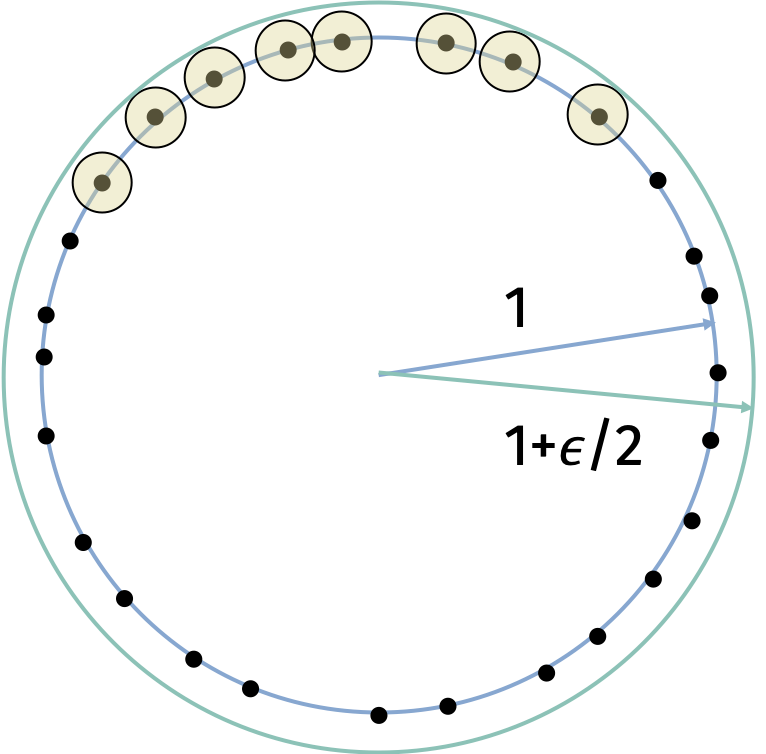
\includegraphics[width=.4\textwidth]{net_argument.png}
	\end{center}

	
	Can place a ball of radius $\epsilon/2$ around each $\bv{w}_i$ without intersecting any other balls. All of these balls live in a ball of radius $1+\epsilon/2$.
\end{frame}

\begin{frame}[t]
	\frametitle{$\epsilon$-net for the sphere}
	Volume of $d$ dimensional ball of radius $r$ is 
	\begin{align*}
		\vol(d,r) = c\cdot r^d,
	\end{align*}
	where $c$ is a constant that depends on $d$, but not $r$.
	\vspace{1em}
	From previous slide we have:
	\begin{align*}
		\vol(d,\epsilon/2) \cdot |N_\epsilon| &\leq \vol(d,1+\epsilon/2) \\  
		|N_\epsilon| &\leq \frac{\vol(d,1+\epsilon/2)}{\vol(d,\epsilon/2)} \\
		&\leq \left(\frac{1+\epsilon/2}{\epsilon/2}\right)^d\leq \left(\frac{3}{\epsilon}\right)^d
	\end{align*}
\end{frame}

\begin{frame} 
	\frametitle{tighter bound}
	You can actually show that $m = O\left(\frac{d + \log(1/\delta)}{\epsilon}\right)$ suffices to be a $d$ dimensional subspace embedding, instead of the bound we proved of $m = O\left(\frac{d\log(1/\epsilon) + \log(1/\delta)}{\epsilon}\right)$.
	
	The trick is to show that a \emph{constant} factor net is actually all that you need instead of an $\epsilon$ factor. 
	\end{frame}

\begin{frame}[t]
	\frametitle{runtime consideration}
	For $\epsilon, \delta = O(1)$, we need $\bs{\Pi}$ to have $m = O(d)$ rows.
	\begin{itemize}
		\item Cost to solve $\|\bv{A}\bv{x} - \bv{b}\|_2^2$: 
		\begin{itemize}
			\item \alert{$O(nd^2)$} time for direct method. Need to compute $(\bv{A}^T\bv{A})^{-1}\bv{A}^T\bv{b}$.
			\item \alert{$O(nd)\cdot \text{(\# of iterations)}$} time for iterative method (GD, AGD, conjugate gradient method).
		\end{itemize}
		\item Cost to solve $\|\bs{\Pi}\bv{A}\bv{x} - \bs{\Pi}\bv{b}\|_2^2$: 
		\begin{itemize}
			\item \alert{$O(d^3)$} time for direct method. 
			\item \alert{$O(d^2)\cdot \text{(\# of iterations)}$} time for iterative method.
		\end{itemize}
	\end{itemize}
\end{frame}

\begin{frame}[t]
	\frametitle{runtime consideration}
	But time to compute $\bs{\Pi}\bv{A}$ is an $(m\times n) \times (n \times d)$ matrix multiply: $O(mnd) = \alert{O(nd^2)}$ \alert{time}!
	
	\begin{center}
		\textbf{Goal}: Develop faster Johnson-Lindenstrauss projections.
		\vspace{.5em}
		
		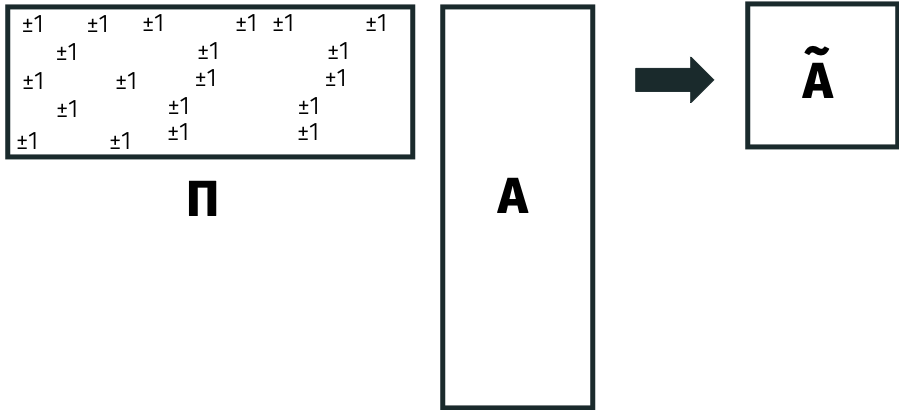
\includegraphics[width=.6\textwidth]{sparseJL.png}
		
		Typically using \emph{sparse} and \emph{structured} matrices.
	
	\end{center}
			\textbf{Next class}: We will describe a construction where $\bs{\Pi}\bv{A}$ can be computed in \alert{$O(nd\log n)$ time}.
\end{frame}

\begin{frame}[t]
	\frametitle{return to single vector problem}
	\textbf{Goal}: Develop methods that reduce a vector $\bv{x}\in \R^n$ down to $m \approx \frac{\log(1/\delta)}{\epsilon^2}$ dimensions in $o(mn)$ time and guarantee:
	\begin{align*}
		(1-\epsilon)\|\bv{x}\|_2^2 \leq \|\bs{\Pi}\bv{x}\|_2^2 \leq (1+\epsilon)\|\bv{x}\|_2^2
	\end{align*}
	\begin{center}
		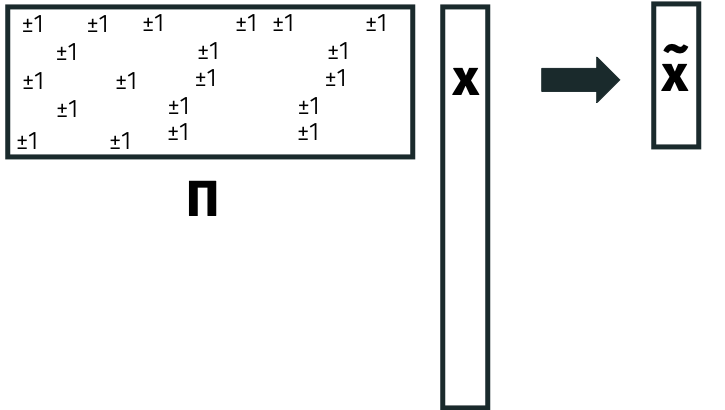
\includegraphics[width=.6\textwidth]{single_vec.png}
	\end{center}
	There is a truly brilliant method that runs in $O(n\log n)$ time. \textbf{Preview:} Will involve Fast Fourier Transform in disguise. 
\end{frame}

%\begin{frame}[t]
%	\frametitle{first attempt}
%	Let $\bs{\Pi}$ be a \alert{random sampling matrix}. Every row contains a value of $s = \sqrt{n/m}$ in a single location, and is zero elsewhere. 
%	
%	\vspace{-1em}
%	\begin{center}
%		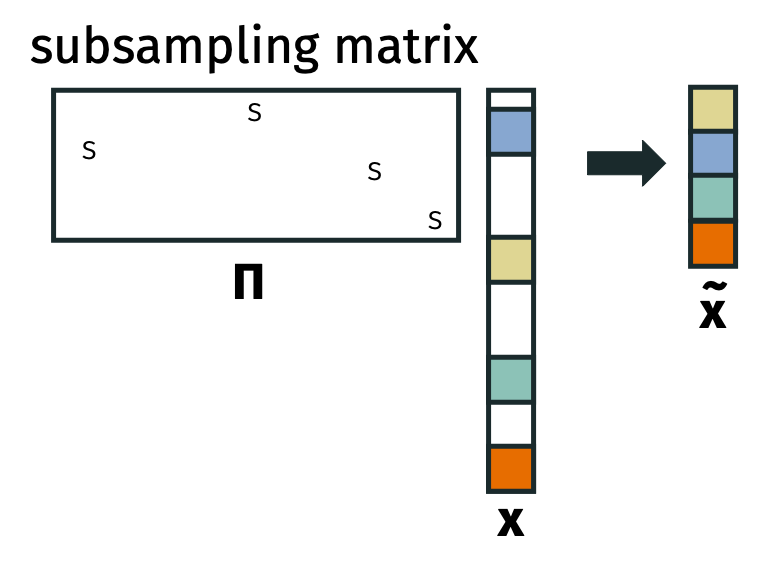
\includegraphics[width=.6\textwidth]{sampling.png}
%	\end{center}
%	\vspace{-7.5em}
%	
%	What's the running time\\
%	to compute $\bs{\Pi} \bv{x}$?
%	\vspace{2em}
%	
%	$\|\bs{\Pi}\bv{x}\|_2^2 = $
%	
%	$\E[\|\bs{\Pi}\bv{x}\|_2^2] = $
%\end{frame}
%
%\begin{frame}[t]
%	\frametitle{first attempt}
%	So $\E\|\bs{\Pi}\bv{x}\|_2^2 = \|\bv{x}\|_2^2$ in expectation. To show it is close with high probability we would need to apply a concentration inequality. How do you think this will work out?
%	\begin{center}
%		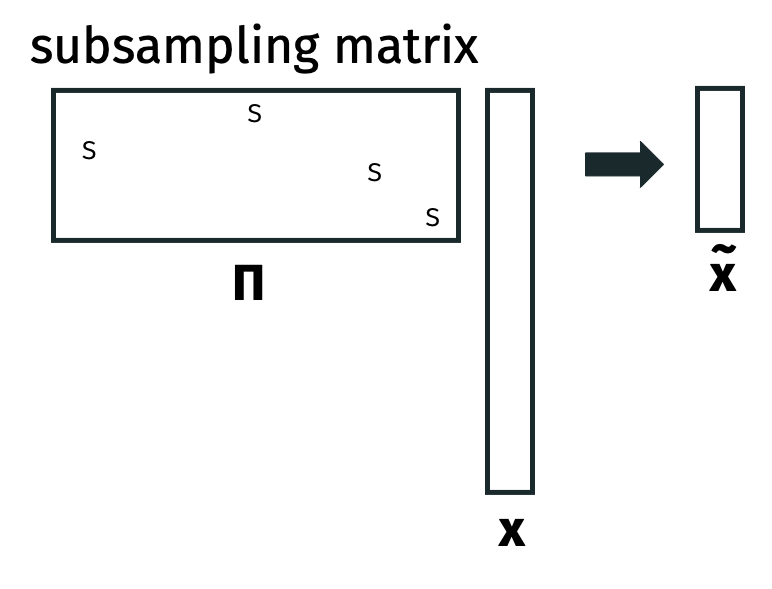
\includegraphics[width=.6\textwidth]{sample_hard.png}
%	\end{center}
%\end{frame}
%
%\begin{frame}[t]
%	\frametitle{variance analysis}	
%	$\|\bs{\Pi}\bv{x}\|_2^2 = $
%	
%	$\sigma^2 = \Var[\|\bs{\Pi}\bv{x}\|_2^2] = $
%	
%	
%	\vspace{8em}
%	Recall Chebyshev's Inequality:
%	\begin{align*}
%		\Pr[\left|\|\bs{\Pi}\bv{x}\|_2^2 - \|\bv{x}\|_2^2\right| \leq 10\cdot \sigma] \leq \frac{1}{100}
%	\end{align*}
%	We want additive error $\left|\|\bs{\Pi}\bv{x}\|_2^2 - \|\bv{x}\|_2^2\right| \leq \epsilon \|\bv{x}\|_2^2$
%\end{frame}	
%
%\begin{frame}[t]
%	\frametitle{variance analysis}	
%	We need to choose $m$ so that:
%	\begin{align*}
%		10\sqrt{\frac{n}{m}}\|\bv{x}\|_4^2 \leq \epsilon \|\bv{x}\|_2^2.
%	\end{align*}
%	How do these two two norms compare?
%	\begin{align*}
%		\|\bv{x}\|_4^2 &= \left(\sum_{i=1}^n x_i^4\right)^{1/2} & \|\bv{x}\|_2^2 &= \sum_{i=1}^n x_i^2
%	\end{align*}
%	Consider 2 extreme cases:
%	\begin{align*}
%		\bv{x} &= \begin{bmatrix}1\\0\\\vdots\\0\end{bmatrix} & \bv{x} &= \begin{bmatrix}1\\1\\\vdots\\1\end{bmatrix}.
%	\end{align*}
%\end{frame}
%
%\begin{frame}[t]
%	\frametitle{variance for smoooth functions}	
%	We need to choose $m$ so that:
%	\begin{align*}
%		\frac{1}{10}\sqrt{\frac{n}{m}}\|\bv{x}\|_4^2 \leq \epsilon \|\bv{x}\|_2^2.
%	\end{align*}
%	Suppose $\bv{x}$ is very evenly distributed. I.e., for all $i\in 1, \ldots, n$,
%	\begin{align*}
%		x_i^2 \leq \frac{c}{n}\sum_{i=1}^n x_i^2 = \frac{c}{n}\|\bv{x}\|_2^2
%	\end{align*}
%	\textbf{Claim:} $\|\bv{x}\|_4^2 \leq \frac{c}{\sqrt{n}} \|\bv{x}\|_2^2$. So $m  = O(c/\epsilon^2)$ samples suffices.\footnote{\footnotesize Using the right Bernstein bound we can prove $m  = O(c\log(1/\delta)/\epsilon^2)$ suffices for failure probability $\delta$.}    
%	\vspace{2em}                    
%\end{frame}
%
%\begin{frame}[t]
%	\frametitle{vector sampling}	
%	So sampling does work to preserve the norm of $\bv{x}$, but only when the vector is relatively ``smooth'' (not concentrated). Do we expect to see such vectors in the wild?
%	
%	\begin{center}
%		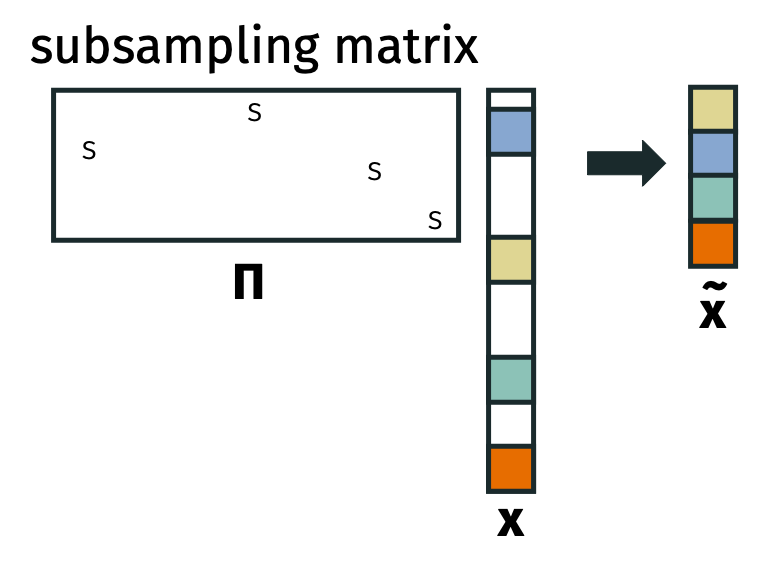
\includegraphics[width=.6\textwidth]{sampling.png}
%	\end{center}
%\end{frame}	
%
%\begin{frame}[t]
%	\frametitle{the fast johnson-lindenstrauss transform}
%	\begin{center}
%		\textbf{Subsampled Randomized Hadamard Transform (SHRT) (Ailon-Chazelle, 2006)}
%	\end{center}
%	\textbf{Key idea:} First multiply $\bv{x}$ by a ``mixing matrix'' $\bv{M}$ which ensures it cannot be too concentrated in one place. 
%	
%	$\bv{M}$ should have the property that $\|\bv{M}\bv{x}\|_2^2 = \|\bv{x}\|_2^2$ exactly, or is very close. Then we will multiply by a subsampling matrix $\bv{S}$ to do the actual dimensionality reduction:
%	\begin{align*}
%		\bs{\Pi}\bv{x} = \bv{SM}\bv{x}
%	\end{align*}
%
%\begin{center}
%	\alert{
%Oh... and $\bv{M}$ needs to be fast to multiply by!}
%\end{center}
%	
%\end{frame}
%
%\begin{frame}[t]
%	\frametitle{the fast johnson-lindenstrauss transform}
%	Good mixing matrices should look random:
%	\begin{center}
%		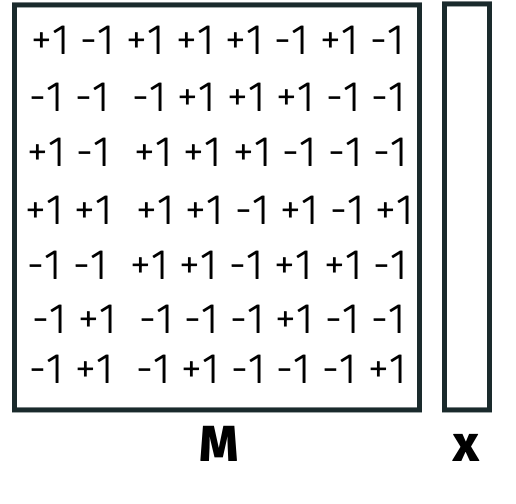
\includegraphics[width=.4\textwidth]{mixing.png}
%		
%		{For this approach to work, we need to be able to compute $\bv{M}\bv{x}$ very quickly.} So we will use a \textbf{\alert{pseudorandom}} matrix instead.
%	\end{center}
%	
%\end{frame}
%
%\begin{frame}[t]
%	\frametitle{the fast johnson-lindenstrauss transform}
%	\begin{center}
%		\textbf{Subsampled Randomized Hadamard Transform (SHRT) (Ailon-Chazelle, 2006)}
%	\end{center}
%	$\bs{\Pi} = \bv{SM}$ where $\bv{M} = \bv{H}\bv{D}$:
%	\begin{itemize}
%		\item $\bv{D} \in n \times n$ is a diagonal matrix with each entry uniform $\pm 1$.
%		\item $\bv{H} \in n \times n$ is a \emph{Hadamard matrix}.
%	\end{itemize}
%	
%	The Hadarmard matrix is an \emph{othogonal} matrix closely related to the discrete Fourier matrix. It has two critical properties: 
%	\begin{enumerate}
%		\item $\|\bv{H}\bv{v}\|_2^2 = \|\bv{v}\|_2^2$ exactly. Thus $\|\bv{H}\bv{D}\bv{x}\|_2^2 = \|\bv{x}\|_2^2$ 
%		\item $\|\bv{H}\bv{v}\|_2^2$ can be computed in $O(n\log n)$ time. 
%	\end{enumerate}
%\end{frame}
%
%\begin{frame}[t]
%	\frametitle{hadamard matrices recursive definition}
%	\textbf{Assume that $n$ is a power of $2$}. For $k = 0, 1, \ldots,$ the $k^\text{th}$ {Hadamard matrix} $\bv{H}_k$ is a $2^k \times 2^k$ matrix defined by:
%	\begin{align*}
%		H_0 &= 1 
%		& H_1 &= \frac{1}{\sqrt{2}}\begin{bmatrix}1 & 1 \\ 1& -1 \end{bmatrix} 
%		& H_2 &= \frac{1}{\sqrt{4}}\begin{bmatrix}1 & 1 & 1& 1 \\ 1 & -1 & 1& -1 \\ 1 & 1 & -1& -1 \\1 & -1 & -1& 1  \end{bmatrix} 
%	\end{align*}
%	\begin{align*}
%		H_k &= \frac{1}{\sqrt{2}}\begin{bmatrix}H_{k-1} & H_{k-1}  \\ H_{k-1} & -H_{k-1}  \end{bmatrix}
%	\end{align*}
%	\begin{center}
%		The $n\times n$ Hadamard matrix has all entries as $\pm \frac{1}{\sqrt{n}}$. 
%	\end{center}
%\end{frame}
%
%\begin{frame}[t]
%	\frametitle{hadamard matrices are orthogonal}
%	\textbf{Property 1}: For any $k = 0, 1, \ldots$, we have $\|\bv{H}_k\bv{v}\|_2^2 = \|\bv{v}\|_2^2$ for all $\bv{v}$. I.e., $\bv{H}_k$ is orthogonal.
%	
%	
%\end{frame}
%
%\begin{frame}[t]
%	\frametitle{hadamard matrices}
%	\textbf{Property 2}: Can compute $\bs{\Pi}\bv{x} = \bv{SHD}\bv{x}$ in $O(n\log n)$ time. 
%	\vspace{14em}
%	
%\end{frame}
%
%\begin{frame}
%	\frametitle{randomized hadamard transform}
%	\textbf{Property 3}: The randomized Hadamard matrix is a good ``mixing matrix'' for smoothing out vectors. 
%	
%	\begin{figure}[h]
%		\centering
%		\begin{subfigure}[t]{0.3\textwidth}
%			\centering
%			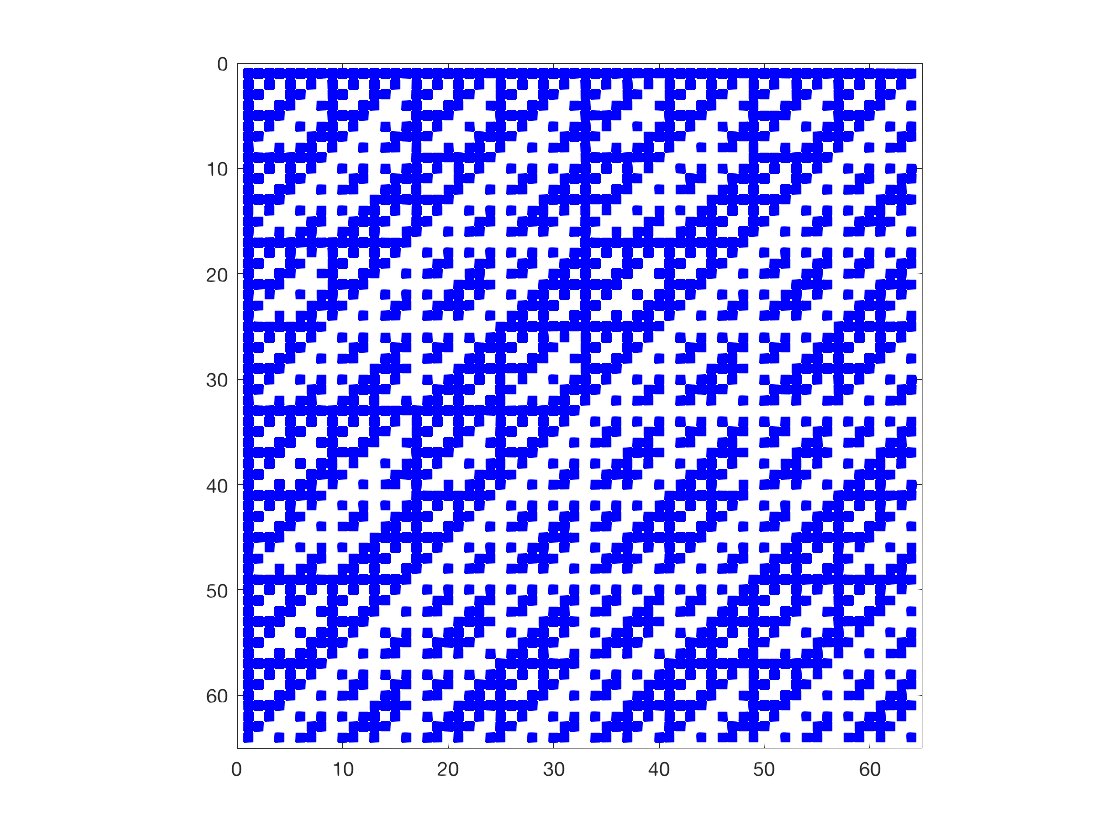
\includegraphics[width=\textwidth]{hadamard.png}
%			\caption{Deterministic Hadamard matrix.}
%		\end{subfigure}
%		\begin{subfigure}[t]{0.3\textwidth}
%			\centering
%			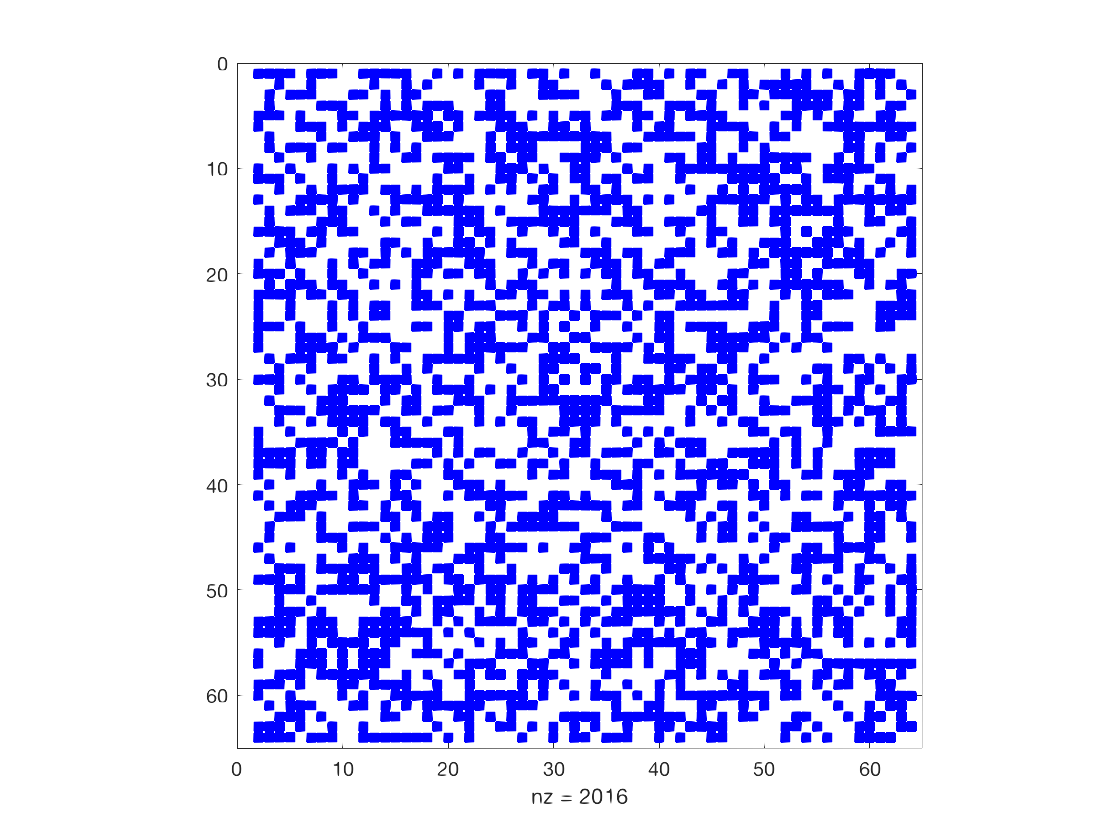
\includegraphics[width=\textwidth]{randomizedHadamard.png}
%			\caption{Randomized Hadamard $\bv{PHD}$.}
%		\end{subfigure}
%		\begin{subfigure}[t]{0.3\textwidth}
%			\centering
%			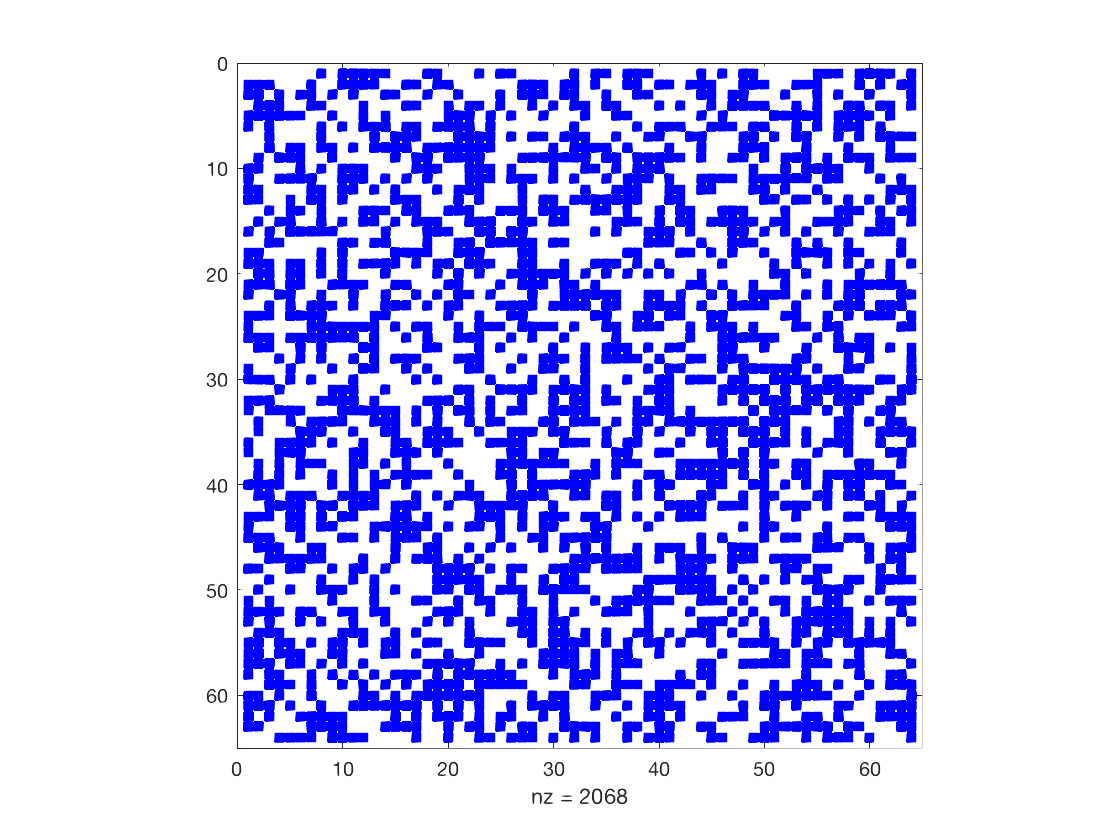
\includegraphics[width=\textwidth]{fullyRandom.png}
%			\caption{Fully random sign matrix.}
%		\end{subfigure}
%		\caption{Blue squares are $1/\sqrt{n}$'s, white squares are $-1/\sqrt{n}$'s.}
%	\end{figure}
%\end{frame}
%
%\begin{frame}[t]
%	\frametitle{randomized hadamard analysis}
%	\begin{lemma}[SHRT mixing lemma]
%		Let $\bv{H}$ be an $(n\times n)$ Hadamard matrix and $\bv{D}$ a random $\pm 1$ diagonal matrix. Let $\bv{z} = \bv{HD}\bv{x}$ for $\bv{x}\in \R^n$. With probability $1-\delta$,
%		\begin{align*}
%			(z_i)^2 \leq \frac{c\log(n/\delta)}{n} \|\bv{z}\|_2^2 
%		\end{align*}
%		for some fixed constant $c$. 
%	\end{lemma}
%	\alert{\textbf{The vector is very close to uniform with high probability}.} As we saw earlier, we can thus argue that $\|\bv{S}\bv{z}\|_2^2 \approx \|\bv{z}\|_2^2$. I.e. that:
%	\begin{align*}
%		\|\bs{\Pi}\bv{x}\|_2^2 = \|\bv{SHD}\bv{x}\|_2^2 \approx \|\bv{x}\|_2^2
%	\end{align*}
%\end{frame}
%
%\begin{frame}[t]
%	\frametitle{johnson-lindenstrauss with shrts}
%	\begin{theorem}[The Fast JL Lemma]
%		Let $\bs{\Pi} = \bv{SHD} \in \R^{m\times n}$ be a subsampled randomized Hadamard transform with $m = O\left(\frac{\log(n/\delta)\log(1/\delta)}{\epsilon^2}\right)$ rows. Then for any fixed $\bv{x}$, 
%		\begin{align*}
%			(1-\epsilon)\|\bv{x}\|_2^2 \leq  \|\bs{\Pi}\bv{x}\|_2^2 \leq (1+\epsilon) \|\bv{x}\|_2^2
%		\end{align*}
%		with probability $(1-\delta)$. 
%	\end{theorem}
%	\begin{center}
%		Very little loss in embedding dimension compared to full random matrix, and $\bs{\Pi}$ can be multiplied by $\bv{x}$ in $O(n\log n)$ (nearly linear) time.
%	\end{center}
%\end{frame}
%
%\begin{frame}[t]
%	\frametitle{randomized hadamard analysis}
%	\textbf{SHRT mixing lemma proof:}
%	Need to prove $(z_i)^2 \leq \frac{c\log(n/\delta)}{n} \|\bv{z}\|_2^2$ \underline{for all $i$}. 
%	
%	Let $\bv{h}_i^T$ be the $i^\text{th}$ row of $\bv{H}$. ${z}_i = \bv{h}_i^T\bv{D}\bv{x}$ where:
%	\begin{align*}
%		\bv{h}_i^T\bv{D} = \frac{1}{\sqrt{n}}\begin{bmatrix} 1 & 1 & \ldots & -1 & -1 \end{bmatrix}
%		\begin{bmatrix} 
%			D_1 &  &  & \\ 
%			& D_2  &  & \\ 
%			& &  \ddots  & \\ 
%			& &   &  D_n \\ 
%		\end{bmatrix}
%	\end{align*}
%	where $D_1, \ldots, D_n$ are random $\pm 1$'s.
%	
%	This is equivalent to
%	\begin{align*}
%		\bv{h}_i^T\bv{D}  = \frac{1}{\sqrt{n}}\begin{bmatrix} R_1 & R_2 & \ldots & R_n \end{bmatrix}, 
%	\end{align*}
%	where $R_1, \ldots, R_n$ are random $\pm 1$'s.
%	
%\end{frame}
%
%\begin{frame}[t]
%	\frametitle{randomized hadamard analysis}
%	So we have, for all $i$,
%	$\bv{z}_i = \bv{h}_i^T\bv{D}\bv{x} = \frac{1}{\sqrt{n}}\sum_{i=1}^n R_i x_i.$
%	
%	\begin{itemize}
%		\item $\bv{z}_i$ is a random variable with mean $0$ and variance $\frac{1}{n}\|\bv{x}\|_2^2$, and is a sum of independent random variables. 
%		\item By Central Limit Theorem, we expect that:
%		\begin{align*}
%			\Pr[|\bv{z}_i| \geq t\cdot \frac{\|\bv{x}\|_2}{\sqrt{n}}] \leq e^{-O(t^2)}. 
%		\end{align*}
%		\item Setting $t = \sqrt{\log(n/\delta)}$, we have for constant $c$, \begin{align*}\Pr\left[|\bv{z}_i| \geq c\sqrt{\frac{\log(n/\delta)}{n}}\|\bv{y}\|_2 \right] \leq \frac{\delta}{n}\end{align*}. 
%		\item Applying a union bound to all $n$ entries of $\bv{z}$ gives the SHRT mixing lemma.
%	\end{itemize}
%\end{frame}
%
%\begin{frame}[t]
%	\frametitle{rademacher concentration}
%	Formally, need to use Bernstein type concentration inequality to prove the bound:
%	\begin{lemma}[Rademacher Concentration]
%		Let ${R}_1, \ldots, R_n$ be Rademacher random variables (i.e. uniform $\pm 1$'s). Then for any vector $\bv{a}\in \R^n$,
%		\begin{align*}
%			\Pr\left[\sum_{i=1}^n R_i a_i \geq t \|\bv{a}\|_2 \right] \leq e^{-t^2/2}.
%		\end{align*}
%	\end{lemma}
%	This is call the \emph{Khintchine Inequality}. It is specialized to sums of scaled $\pm 1$'s, and is a bit tighter and easier to apply than using a generic Bernstein bound.
%\end{frame}
%
%\begin{frame} 
%	\frametitle{finishing up}
%	With probability $1-\delta$, we have that all $\bv{z}_i \leq \sqrt{\frac{c\log(n/\delta)}{n}}\|\bv{c}\|_2$. 
%	
%	As shown earlier, we can thus guarantee that:
%	\begin{align*}
%		(1-\epsilon)\|\bv{z}\|_2^2 \leq \|\bv{S}\bv{z}\|_2^2 \leq (1+\epsilon)\|\bv{z}\|_2^2
%	\end{align*}
%	as long as $\bv{S}\in \R^{m\times n}$ is a random sampling matrix with
%	\begin{align*}
%		m = O\left(\frac{\log(n/\delta)\log(1/\delta)}{\epsilon^2}\right) \text{ rows}. 
%	\end{align*}
%	
%	$\|\bv{S}\bv{z}\|_2^2 = \|\bv{SHD}\bv{x}\|_2^2 = \|\bs{\Pi}\bv{x}\|_2^2$ and $\|\bv{z}\|_2^2 = \|\bv{x}\|_2^2$, so we are done. 
%\end{frame}
%
%\begin{frame}[t]
%	\frametitle{johnson-lindenstrauss with SHRTs}
%	\begin{theorem}[The Fast JL Lemma]
%		Let $\bs{\Pi} = \bv{SHD} \in \R^{m\times n}$ be a subsampled randomized Hadamard transform with $m = O\left(\frac{\log(n/\delta)\log(1/\delta)}{\epsilon^2}\right)$ rows. Then for any fixed $\bv{x}$, 
%		\begin{align*}
%			(1-\epsilon)\|\bv{x}\|_2^2 \leq  \|\bs{\Pi}\bv{x}\|_2^2 \leq (1+\epsilon) \|\bv{x}\|_2^2
%		\end{align*}
%		with probability $(1-\delta)$. 
%	\end{theorem}
%	
%	\textbf{Upshot for regression:} Compute $\bs{\Pi}\bv{A}$ in \alert{$O(nd\log n)$ time} instead of $O(nd^2)$ time. Compress problem down to $\bv{\~ A}$ with $O(d^2)$ dimensions. 
%\end{frame}
%
%\begin{frame}[t]
%	\frametitle{brief comment on other methods}
%	$O(nd\log n)$ is nearly linear in the size of $\bv{A}$ when $\bv{A}$ is dense. 
%	\vspace{1em}
%	
%	\textbf{Clarkson-Woodruff 2013, STOC Best Paper}: Possible to compute $\bv{\~{A}}$ with $\poly(d)$ rows in:
%	\begin{align*}
%		O\left(\nnz(\bv{A})\right) \text{ time.}
%	\end{align*}
%	$\bs{\Pi}$ is chosen to be an ultra-sparse random matrix. Uses totally different techniques (you can't do JL + $\epsilon$-net).
%	
%	Lead to a whole close of matrix algorithms (for regression, SVD, etc.) which run in time:
%	\begin{align*}
%		O\left(\nnz(\bv{A})\right)  + \poly(d,\epsilon).
%	\end{align*}
%\end{frame}
%
%\begin{frame}[t]
%	\frametitle{what were ailon and chazelle thinking?}
%	Simple, inspired algorithm that has been used for accelerating:
%	\begin{columns}
%		\begin{column}{.5\textwidth}
%			\footnotesize{
%				\begin{itemize}
%					\item Vector dimensionality reduction
%					\item Linear algebra
%					\item Locality sensitive hashing (SimHash)
%					\item Randomized kernel learning methods (we will discuss after Thanksgiving)
%				\end{itemize}
%			}
%		\end{column}
%		\begin{column}{.5\textwidth}
%			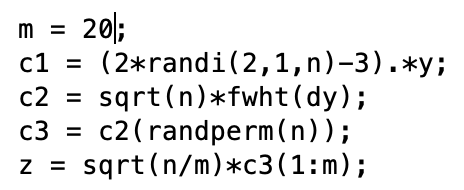
\includegraphics[width=\textwidth]{fastJL.png}
%		\end{column}
%	\end{columns}
%\end{frame}
%
%\begin{frame}
%	\frametitle{what were ailon and chazelle thinking?}
%	The \emph{Hadamard Transform} is closely related to the \emph{Discrete Fourier Transform}.
%	\begin{align*}
%		\bv{F}_{j,k} &= e^{-2\pi i \frac{j\cdot k}{n}}, & \bv{F}^*\bv{F} &= \bv{I}.
%	\end{align*}
%	\begin{center}
%		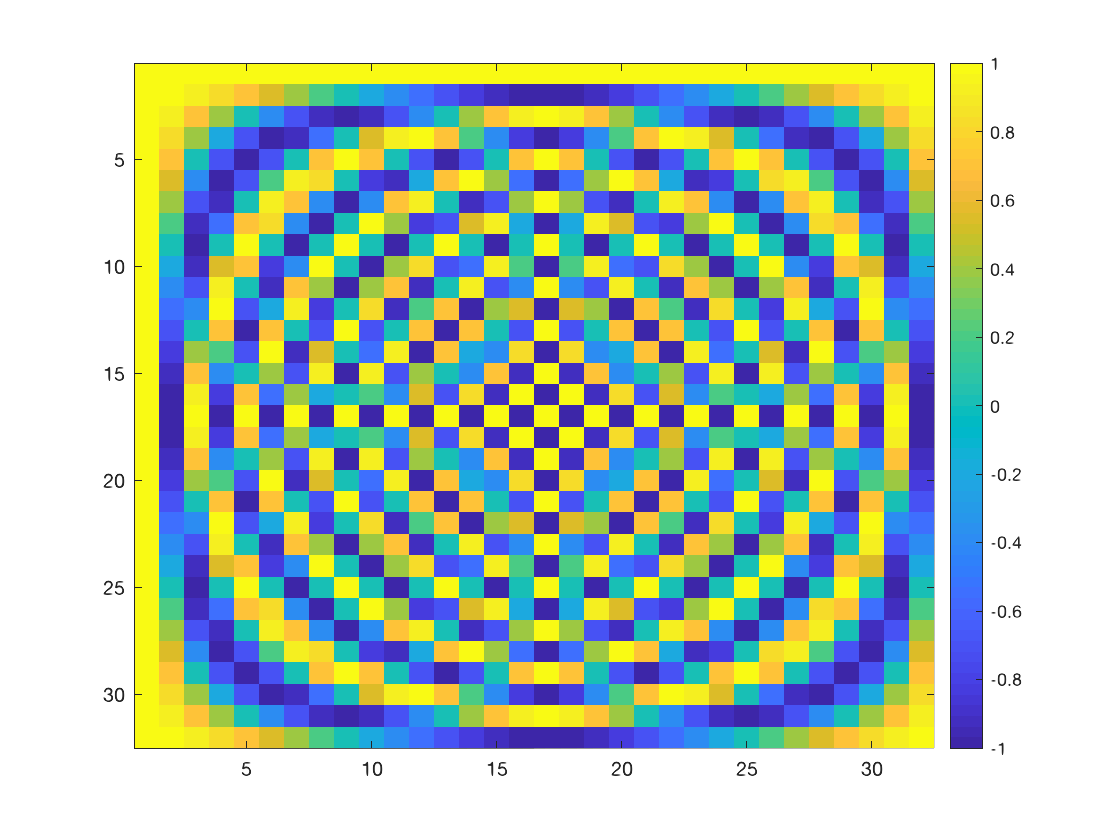
\includegraphics[width=.4\textwidth]{dft.png}
%		\vspace{-1em}
%		
%		Real part of $\bv{F}_{j,k}$.
%	\end{center}
%	
%	$\bv{F}\bv{y}$ computes the Discrete Fourier Transform of the vector $\bv{y}$. Can be computed in $O(n\log n)$ time using a divide and conquer algorithm (the Fast Fourier Transform).
%\end{frame}
%
%\begin{frame}
%	\frametitle{the uncertainty principal}
%	\textbf{The Uncertainty Principal (informal):} A function and it's Fourier transform cannot both be concentrated. 
%	\vspace{1em}
%	\begin{columns}
%		\begin{column}{.5\textwidth}
%			\centering
%			\includegraphics[width=.8\textwidth]{y.png}
%			
%			Vector $\bv{y}.$
%		\end{column}
%		\begin{column}{.5\textwidth}
%			\centering
%			\includegraphics[width=.8\textwidth]{Fy.png}
%			
%			Fourier transform $\bv{Fy}.$
%		\end{column}
%	\end{columns}
%\end{frame}
%
%\begin{frame}[t]
%	\frametitle{sparse recovery/compressed sensing}
%	\begin{center}
%		What do we know?
%	\end{center}
%\end{frame}
%
%\begin{frame}
%	\frametitle{the uncertainty principal}
%	Sampling does not preserve norms, i.e. $\|\bv{S}\bv{y}\|_2 \not\approx \|\bv{y}\|_2$ when $\bv{y}$ has a few large entries. 
%	
%	Taking a Fourier transform exactly eliminates this hard case, without changing $\bv{y}$'s norm.
%	
%	\begin{center}
%		One of the central tools in the field of \alert{\textbf{sparse recovery}} aka \alert{\textbf{compressed sensing.}}
%	\end{center}
%\end{frame}
\end{document} 




